\documentclass{beamer}

\mode<presentation>





\usetheme{Frankfurt}%
\usecolortheme{seagull}
\logo{\includegraphics[height=.25in]{clarksonGreen}}

\definecolor{garnet}{RGB}{136,0,0}
%\definecolor{clarksonGreen}{RGB}{0,71,28}
\definecolor{clarksonGreen}{RGB}{0,52,21}
\setbeamercolor{palette primary}{fg=clarksonGreen,bg=white}
\setbeamercolor{palette secondary}{fg=clarksonGreen,bg=white}
\setbeamercolor{palette tertiary}{fg=clarksonGreen,bg=white}
\setbeamercolor{palette quaternary}{bg=clarksonGreen,fg=white}
\setbeamercolor{block title}{fg=black,bg=black!15}
\setbeamercolor{block body}{fg=black,bg=black!10}
\setbeamercolor{titlelike}{bg=clarksonGreen,fg=white} % parent=palette quaternary}

\newcommand{\half}{\mbox{$\frac{1}{2}$}}
\newcommand{\deltat}{\mbox{$\triangle t$}}
\newcommand{\deltax}{\mbox{$\triangle x$}}
\newcommand{\deltay}{\mbox{$\triangle y$}}

\newcommand{\deriv}[2]{\frac{d}{d#2}#1}
\newcommand{\derivTwo}[2]{\frac{d^2}{d#2^2}#1}

\newcommand{\lp}{\left(}
\newcommand{\rp}{\right)}


\includeonlylecture{Inverse-Laplace-Transforms}
\includeonly{week13-Day1}


\begin{document}


\part{Introduction}
\lecture{Introduction}{Introduction}

\documentclass{beamer}

\mode<presentation>





\usetheme{Frankfurt}%
\usecolortheme{seagull}
\logo{\includegraphics[height=.25in]{clarksonGreen}}

\definecolor{garnet}{RGB}{136,0,0}
%\definecolor{clarksonGreen}{RGB}{0,71,28}
\definecolor{clarksonGreen}{RGB}{0,52,21}
\setbeamercolor{palette primary}{fg=clarksonGreen,bg=white}
\setbeamercolor{palette secondary}{fg=clarksonGreen,bg=white}
\setbeamercolor{palette tertiary}{fg=clarksonGreen,bg=white}
\setbeamercolor{palette quaternary}{bg=clarksonGreen,fg=white}
\setbeamercolor{block title}{fg=black,bg=black!15}
\setbeamercolor{block body}{fg=black,bg=black!10}
\setbeamercolor{titlelike}{bg=clarksonGreen,fg=white} % parent=palette quaternary}

\newcommand{\half}{\mbox{$\frac{1}{2}$}}
\newcommand{\deltat}{\mbox{$\triangle t$}}
\newcommand{\deltax}{\mbox{$\triangle x$}}
\newcommand{\deltay}{\mbox{$\triangle y$}}

\newcommand{\deriv}[2]{\frac{d}{d#2}#1}
\newcommand{\derivTwo}[2]{\frac{d^2}{d#2^2}#1}

\newcommand{\lp}{\left(}
\newcommand{\rp}{\right)}



\begin{document}

\title{Ordinary Differential Equations}
\subtitle{Math 232 - Week 1, Day 1}

\author{Kelly Black}
\institute{Clarkson University}
\date{28 Aug 2011}

\begin{frame}
  \titlepage
\end{frame}

\begin{frame}
  \frametitle{Outline}
  \tableofcontents[pausesection,hideallsubsections]
\end{frame}


\section{What is a Differential Equation}


\begin{frame}
  \frametitle{What is a DE?}

  Given
  \begin{eqnarray*}
    y' & = & y,
  \end{eqnarray*}
  what is $y(x)=?$

  \begin{eqnarray*}
    \deriv{y(x)}{x} & = & y(x)
  \end{eqnarray*}

\end{frame}


\begin{frame}
  Given
  \begin{eqnarray*}
    y'' + 3y' +2y & = & 0
  \end{eqnarray*}

  what is $y(x)$?

\end{frame}

\begin{frame}
  \frametitle{Notation}
  \begin{eqnarray*}
    \dot{y} & = & \deriv{y}{t} \\
    \ddot{y} & = & \derivTwo{y}{t} \\
    y' & = & \mathrm{depends.... usually ~~} \deriv{y(x)}{x} \\
    y'' & = & \derivTwo{y(x)}{x}
  \end{eqnarray*}
\end{frame}

\begin{frame}
  \frametitle{Nomenclature}
  
  \vfill

  $\deriv{y}{x}$ - then ``ordinary differential equation.''

  \vfill

  $\frac{\partial y}{\partial x}$ - then ``partial differential
  equation.''

  \vfill

  Order is the highest number of derivatives:
  \begin{eqnarray*}
    y'' - 3 y' + 2y & = & 0, \mathrm{second~order} \\
    y'  & = & 4y, \mathrm{first~order} 
  \end{eqnarray*}

  \vfill


\end{frame}

\section{Modeling}


\begin{frame}
  \frametitle{Modeling}

  Why bother?

  Many ``mathematical models'' provide a relationship between rates.

  ex: Newton's Second Law, ``$\vec{F} = m \vec{a}$'' In 1 dimension:
  \begin{eqnarray*}
    m\mathrm{~(acceleration)} & = & \sum_i \lp F_x \rp_i, \\
    m \ddot{x} & = & \sum_i \lp f_x \rp_i
  \end{eqnarray*}

  
\end{frame}


\begin{frame}
  \frametitle{Circuit}
  
  The voltage across a resistor is proportional to the current flowing
  through it.

  There is some number, R, where
  \begin{eqnarray*}
    V & = & IR
  \end{eqnarray*}
\end{frame}

\begin{frame}
  \frametitle{Proportionality}
  
  If $a$ is proportional to $b$ then there is a constant, $k$, where 
  \begin{eqnarray*}
    a  & = & k \cdot b
  \end{eqnarray*}

  if $a$ is inversely proportional to $b$ then there is a constant $c$
  where 
  \begin{eqnarray*}
    a & = & c \frac{1}{b}
  \end{eqnarray*}
\end{frame}

\end{document}

% LocalWords:  Clarkson pausesection hideallsubsections


\part{Solutions-to-DEs}
\lecture{Solutions to DEs}{Solutions-to-DEs}


\title{Ordinary Differential Equations}
\subtitle{Math 232 - Week 1, Day 2}

\author{Kelly Black}
\institute{Clarkson University}
\date{30 Aug 2011}

\begin{frame}
  \titlepage
\end{frame}

\begin{frame}
  \frametitle{Outline}
  \tableofcontents[pausesection,hideallsubsections]
\end{frame}


\section{Solutions to DEs}


\begin{frame}
  \frametitle{What is a solution to a DE?}

  \begin{eqnarray*}
    y' & = & y
  \end{eqnarray*}

  Solution: $y=3e^t$

  \uncover<2->{
    Check: 
    \begin{eqnarray*}
      y' & = & 3e^t \\
      y  & = & 3e^t
    \end{eqnarray*}

    The same!
  }

\end{frame}


\begin{frame}
  \frametitle{What is a solution to a DE?}

  \begin{eqnarray*}
    y' & = & y
  \end{eqnarray*}

  Solution: $y=2e^t$

  \uncover<2->{
    Check: 
    \begin{eqnarray*}
      y' & = & 2e^t \\
      y  & = & 2e^t
    \end{eqnarray*}

    The same!
  }


\end{frame}


\begin{frame}
  \frametitle{What is a solution to a DE?}

  \begin{eqnarray*}
    y' & = & y, \\
    y(0) & = & 1
  \end{eqnarray*}

  Neither is a solution! 

  \uncover<2->{
    Solution: $y=e^t$

    Check: 
    \begin{eqnarray*}
      y' & = & e^t \\
      y  & = & e^t \\
      y(0) & = & 1
    \end{eqnarray*}

    This is the solution.
  }

\end{frame}


\begin{frame}
  \frametitle{What is a solution to a DE?}

  Show that 
  \begin{eqnarray*}
    y & = & 3 e^{2t} - \half
  \end{eqnarray*}
  is a solution to
  \begin{eqnarray*}
    y' & = & 2y + 1.
  \end{eqnarray*}

  \uncover<2->{
    \begin{eqnarray*}
      y' & = & 6 e^{2t} \\
      2y+1 & = & 2(3 e^{2t} - \half) +1 \\
      & = & 6 e^{2t}
    \end{eqnarray*}
  }


\end{frame}


\begin{frame}
  \frametitle{What is a solution to a DE?}

  Show that 
  \begin{eqnarray*}
    y & = & \half e^{2t} - \half
  \end{eqnarray*}
  is a solution to
  \begin{eqnarray*}
    y' & = & 2y + 1, \\
    y(0) & = & 0.
  \end{eqnarray*}

  \uncover<2->{
    \begin{eqnarray*}
      y' & = & e^{2t} \\
      2y+1 & = & 2(\half e^{2t} - \half) +1 \\
      & = & e^{2t} \\
      y(0) & = & 0
    \end{eqnarray*}
  }



\end{frame}


\section{Slope Fields}

\begin{frame}
  \frametitle{What is the derivative?}

  The derivative is the slope of the tangent line.

  \begin{tabular}{lll}
    if y'=2 & slope=2 & (inc) \\
    if y'=3 & slope=3 & (inc) \\
    if y'=-2 & slope=-2 & (dec) \\
  \end{tabular}


\end{frame}


\begin{frame}
  \frametitle{Example}

  \begin{eqnarray*}
    y' & = & 5t + 3, \\
    \int y' ~ dt & = & \int 5t + 3 ~ dt \\
    \uncover<2->{y & = & \frac{5}{2} t^2 + 3t + C}
  \end{eqnarray*}

  We get a ``family of solutions.'' 

  If $y(0)=2$ then
  \begin{eqnarray*}
    y(0) & = & \frac{5}{2} (0)^2 + 3(0) + C, \\
    2    & = & C
  \end{eqnarray*}


\end{frame}


\begin{frame}
  \frametitle{Slope Fields}

  Given the differential equation can we predict the \textit{general
    behavior} of the solution? (Qualitative behavior)

  If we have 
  \begin{eqnarray*}
    y' & = & f(t,y),
  \end{eqnarray*}
  then if we know that the function goes through a point, $t=a$ and
  $y(a)=v$, then we can calculate the slope of the tangent line.

\end{frame}


\begin{frame}
  \frametitle{Example}

  \vspace*{-4em}

  \begin{eqnarray*}
    y' & = & 2y
  \end{eqnarray*}

  At $t=3$ if you happen to know that $y=4$ then the slope is 2(4)=8.

  At $t=3$ if you happen to know that $y=5$ then the slope is 2(5)=10.

  \includegraphics[height=4cm]{week1Day2SlopeField}

  A direction field is a collection of segments that indicate the
  tangent lines. 
  
\end{frame}


\begin{frame}
  \frametitle{Example}

  \vspace*{-4em}

  \begin{eqnarray*}
    y' & = & y - t
  \end{eqnarray*}

  \includegraphics[height=5cm]{week1Day2SlopeField2}

  Tools:
  \begin{itemize}
  \item A ``stationary point'' is a point where $y'=0$.
  \item An isocline is a curve where $y'$ is equal to a constant.
  \end{itemize}

\end{frame}


\begin{frame}
  \frametitle{Example}

  \vspace*{-4em}

  \begin{eqnarray*}
    y' & = & y^2 - 3y
  \end{eqnarray*}

  \includegraphics[height=5cm]{week1Day2SlopeField3}

  Definition: An equilibrium solution is a value for which the
  solution does not change in time.

  \uncover<2->{$y(t)=0$ and $y(t)=3$ are equilibrium solutions.}

\end{frame}

\section{Stability}

\begin{frame}
  \frametitle{Stability}

  \begin{itemize}
  \item An \textit{equilibrium solution} is \textbf{stable} if values
    of the solution tend to stay close to it as $t$ increases.
  \item An \textit{equilibrium solution} is \textbf{unstable} if
    values of the solution tend to move away from it as $t$ increases.
  \end{itemize}

  In the previous example $y=0$ is stable while $y=3$ is unstable.

\end{frame}



% LocalWords:  Clarkson pausesection hideallsubsections isocline


\part{Separable-Equations}
\lecture{Separable Equations}{Separable-Equations}

\part{Separable-Equations}
\lecture{Separable Equations}{Separable-Equations}
\section{Separable Equations}


\title{Ordinary Differential Equations}
\subtitle{Math 232 - Week 1, Day 3}
\date{2 Sep 2011}

\begin{frame}
  \titlepage
\end{frame}

\begin{frame}
  \frametitle{Outline}
  \tableofcontents[pausesection,hideothersubsections]
\end{frame}


\subsection{The Chain Rule}


\begin{frame}
  \frametitle{Finding Solutions}

  How do we find a solution to a DE?

  \uncover<2->{Depends!}


\end{frame}


\begin{frame}
  \frametitle{The Chain Rule}

  \begin{eqnarray*}
    \int \lp 1 + \ln(t) \rp \frac{1}{t} ~ dt & = & ?
  \end{eqnarray*}

  \uncover<2->{
    Let $u=1+\ln(t)$ then $du=\frac{1}{t}.$
  }

  \uncover<3-> {
    \begin{eqnarray*}
      \int \lp 1 + \ln(t) \rp \frac{1}{t} ~ dt & = & \int u ~ du \\
      & = & \half u^2 + C \\
      & = & \half \lp 1+\ln(t) \rp^2 + C
    \end{eqnarray*}
  }


\end{frame}

\begin{frame}
  \frametitle{The Chain Rule}

  \begin{eqnarray*}
    \int \lp 1 + \ln(t) \rp \frac{1}{t} ~ dt & = & ?
  \end{eqnarray*}

  \uncover<2->{
    Let $y=1+\ln(t)$ then $dy=\frac{1}{t}.$
  }

  \uncover<3-> {
    \begin{eqnarray*}
      \int \lp 1 + \ln(t) \rp \frac{1}{t} ~ dt & = & \int y ~ dy \\
      & = & \half y^2 + C \\
      & = & \half \lp 1+\ln(t) \rp^2 + C
    \end{eqnarray*}
  }


\end{frame}

\begin{frame}
  \frametitle{The Chain Rule}
  \begin{eqnarray*}
    \int f(y) y' ~ dt & = & \int f(y) ~ dy
  \end{eqnarray*}

  So what?

\end{frame}


\begin{frame}
  \frametitle{A Differential Equation}
  
  \begin{eqnarray*}
    y' & = & 2y
  \end{eqnarray*}

  What is $y$?

  \uncover<2->{
    Note:
    \begin{eqnarray*}
      \frac{1}{y} y' & = & 2
    \end{eqnarray*}
    I can get all the ``$y$''s on the left and the ``t''s on the
    right.
  }

\end{frame}

\subsection{Separable Equations}

\begin{frame}
  \frametitle{Separable Equations}

  Definition: A \textbf{separable differential equation} is an
  equation that can be expressed in the form 
  \begin{eqnarray*}
    y' & = & f(t) g(y).
  \end{eqnarray*}

  In our example:
  \begin{eqnarray*}
    y' & = & 2y \\
    f(t) & = & 2 \\
    g(y) & = & y
  \end{eqnarray*}

\end{frame}


\begin{frame}
  \frametitle{Solving Our Example}

  \begin{eqnarray*}
    y' & = & 2y \\
    \frac{1}{y} y' & = & 2, \\
    \uncover<2->{
      \int \frac{1}{y} y' ~ dt & = & \int 2 ~ dt \\
      \int \frac{1}{y} ~ dy & = & \int 2 ~ dt } \\
    \uncover<3->{
      \ln(y) & = & 2t + C } \\
    \uncover<4->{
      y & = & e^{2t + C} \\
      y & = & e^{2t} \cdot e^C \\
      y & = & k e^{2t}
    }
  \end{eqnarray*}

\end{frame}


\begin{frame}
  \frametitle{In General}

  \begin{eqnarray*}
    y' & = & f(t) g(y) \\
    \frac{1}{g(y)} y' & = & f(t) \\
    \int \frac{1}{g(y)} y' ~ dt & = & \int f(t) ~ dt \\
    \int \frac{1}{g(y)} ~ dy & = & \int f(t) ~ dt 
  \end{eqnarray*}

  \begin{itemize}
  \item Solve the integrals
  \item Solve for $y$ (if possible)
  \end{itemize}


\end{frame}


\begin{frame}
  \frametitle{Example}

  \begin{eqnarray*}
    y' & = & \frac{t}{y+y^2} \\
    \uncover<2->{
      \lp y + y^2 \rp y' & = & t } \\
    \uncover<3->{
      \int \lp y + y^2 \rp y' ~ dt & = & \int t ~ dt \\
      \int \lp y + y^2 \rp ~ dy & = & \int t ~ dt } \\
    \uncover<4->{
      \half y^2 + \frac{1}{3} y^3 & = & \half t^2 + C
    }
  \end{eqnarray*}

  \uncover<5->{
    Cannot solve explicitly for $y(t)$!
  }

\end{frame}


\begin{frame}
  \frametitle{Example}

  \begin{eqnarray*}
    y' & = & 3y + t
  \end{eqnarray*}

  \uncover<2-> { Not separable! }

\end{frame}


\begin{frame}
  \frametitle{Example}

  \begin{eqnarray*}
    y' & = & y^2 + 1 \\
    \uncover<2->{
      \frac{1}{y^2 + 1} y' & = & 1 } \\
    \uncover<3->{
      \int \frac{1}{y^2 + 1} y' ~ dt  & = & \int 1 ~ dt \\
      \int \frac{1}{y^2 + 1}  ~ dy  & = & \int 1 ~ dt } \\
    \uncover<4->{
      \arctan(y) & = & t + C } \\
    \uncover<5->{
      y & = & \tan(t+C)}
  \end{eqnarray*}

\end{frame}


\begin{frame}
  \frametitle{Example}

  \begin{eqnarray*}
    y' & = & yt + t \\
    \uncover<2->{
      y' & = & t(y+1) }\\
    \uncover<3->{
      \int \frac{1}{y+1} y' ~ dt & = & \int t ~ dt \\
      \int \frac{1}{y+1} ~ dy & = & \int t ~ dt \\
    }
    \uncover<4->{
      \ln(y+1) & = & \half t^2 + C }\\
    \uncover<5->{
      y+1 & = & e^{\half t^2 + C} \\
      y+1 & = & e^{\half t^2}e^{C} \\
      y+1 & = & k e^{\half t^2} \\
      y = ke^{\half t^2} - 1 }
  \end{eqnarray*}

\end{frame}


\begin{frame}
  \frametitle{Example}

  \begin{eqnarray*}
    y' & = & \cos(ty) 
  \end{eqnarray*}

  \uncover<2->{Not Separable!}

\end{frame}


\begin{frame}
  \frametitle{Example}

  \begin{eqnarray*}
    y' & = & \frac{t}{y}, ~~~ y(0)=2 \\
    \uncover<2->{
      y y' & = & t } \\
    \uncover<3->{
      \int y y' ~ dt & = & \int t ~ dt } \\
    \uncover<4->{
      \half y^2 & = & \half t^2 + C \\
      y^2 & = & t^2 + k } \\
    \uncover<5->{
      2^2 & = & 0 + k \\
      k   & = & 4 \\
      y & = & \pm \sqrt{t^2+4} } \\
    \uncover<6->{
      \mathrm{Must ~ be ~ positive!} \\
      y & = & \sqrt{t^2+4} }
  \end{eqnarray*}

  \uncover<6->{
    See example 4 in the book.
  }

\end{frame}


\begin{frame}
  \frametitle{Example}

  \begin{eqnarray*}
    ty' & = & y^2 t^2 + 1 \\
    \uncover<2->{
      y'  & = & y^2 t + \frac{1}{t} }
  \end{eqnarray*}

  \uncover<3->{Not separable!}

\end{frame}


\begin{frame}
  \frametitle{Example}

  \begin{eqnarray*}
    t y' & = & y^2+1 \\
    \uncover<2->{
      \frac{y'}{y^2+1} & = & \frac{1}{t} } \\
    \uncover<3->{
      \int \frac{y'}{y^2+1} ~ dt & = & \int \frac{1}{t} ~ dt \\
      \int \frac{1}{y^2+1} ~ dy & = & \int \frac{1}{t} ~ dt } \\
    \uncover<4->{
      \arctan(y) & = & \ln(t)+C } \\
    \uncover<5->{
      y & = & \tan(\ln(t)+C)}
  \end{eqnarray*}





\end{frame}


\begin{frame}
  \frametitle{Example}

  \vspace*{-3em}
  \begin{eqnarray*}
    y' & = & \sec(y) t^2 + \sec(y) \sin(4t) \\
    \uncover<2->{
      y' & = & \sec(y) \lp t^2 + \sin(4t) \rp } \\
    \uncover<3->{
      \frac{y'}{\sec(y)} & = & t^2 + \sin(4t) } \\
    \uncover<4->{
      \int \frac{y'}{\sec(y)} ~ dt & = & \int t^2 + \sin(4t) ~ dt \\
      \int \frac{1}{\sec(y)} ~ dy & = & \int t^2 + \sin(4t) ~ dt }\\
    \uncover<5->{
      \int \cos(y) ~ dy & = & \int t^2 + \sin(4t) ~ dt } \\ 
    \uncover<6->{
      \sin(y) & = & \frac{1}{3} t^3 - \frac{1}{4} \cos(4t) + C } \\
    \uncover<7->{
      y & = & \arcsin\lp\frac{1}{3} t^3 - \frac{1}{4} \cos(4t) + C\rp } \\
  \end{eqnarray*}

  \uncover<8->{This is problematic!}

\end{frame}
 


% LocalWords:  Clarkson pausesection hideothersubsections




% %%%%%%%%%%%%%%%%%%%%%%%%%%%%%%%%%%%%%%%%%%%%%%%%%%%%%%%%%%%%

\part{Linear-Equations}
\lecture{Linear Equations}{Linear-Equations}

\part{Linear-Equations}
\lecture{Linear Equations}{Linear-Equations}


\title{Ordinary Differential Equations}
\subtitle{Math 232 - Week 2, Day 1}

\author{Kelly Black}
\institute{Clarkson University}
\date{5 Sep 2011}

\begin{frame}
  \titlepage
\end{frame}

\begin{frame}
  \frametitle{Outline}
  \tableofcontents[pausesection,hideallsubsections]
\end{frame}


\section{Linear Equations}


\begin{frame}
  \frametitle{Linear Equations}

  If we have variables $x_1$, $x_2$, \ldots, $x_n$ then an equation of
  the form
  \begin{eqnarray*}
    a_1 x_1 + a_2 x_2 + \cdots + a_n x_n & = & c,
  \end{eqnarray*}
  where $a_1$, $a_2$, \ldots, $a_n$, and $c$ are constants, is a
  \textbf{linear equation}.

  if $c$ is zero the equation is \textbf{homogeneous}.

\end{frame}


\begin{frame}
  \frametitle{Linear Equations}

  \begin{eqnarray*}
    3 x_1 + 4 x_2 = 5 & & \uncover<2->{\mathrm{Linear}} \\
    3 x_1 + 4 x^3_2 = 5 & & \uncover<3->{\mathrm{Not~Linear}} \\
    3 \sqrt{x_1} + 4 x_2 = 5 & & \uncover<4->{\mathrm{Not~Linear}} \\
  \end{eqnarray*}


\end{frame}


\begin{frame}
  \frametitle{Linear Differential Equations}

  In the context of DEs an equation is linear if it is in the form 
  \begin{eqnarray*}
    a_0(t) y(t) + a_1(t) \frac{d}{dt}y(t) + \cdots +
    a_n(t) \frac{d^n}{dt^n}y(t) & = & f(t).
  \end{eqnarray*}

  if $f(t)$ is zero the equation is homogeneous.

\end{frame}


\begin{frame}
  \frametitle{Example}

  \vspace*{-3em}
  \begin{eqnarray*}
    3t y + y' - \sin(t) y'' & = & \ln(t)
  \end{eqnarray*}
  \centerline{\uncover<2->{Linear!}}

  \begin{eqnarray*}
    3t \sqrt{y} + y' - \sin(t) y'' & = & \ln(t)
  \end{eqnarray*}
  \centerline{\uncover<3->{Not Linear!}}

  \begin{eqnarray*}
    4 y + 3 y' -  y'' & = & 0
  \end{eqnarray*}
  \centerline{\uncover<4->{Linear, \textbf{constant coefficient}, and homogeneous}}

  Recognizing the form is the hardest part!

\end{frame}

\section{Solutions to Differential Equations}

\begin{frame}
  \frametitle{Solutions to Differential Equations}

  If an equation is linear and homogeneous then:
  \begin{itemize}
  \item If $y_1(t)$ is a solution, and
  \item if $y_2(t)$ is a solution
  \end{itemize}

  then, 
  \begin{eqnarray*}
    y_1(t) + y_2(t)
  \end{eqnarray*}
  is a solution.

  Also if $C_1$ and $C_2$ are constants then
  \begin{eqnarray*}
    C_1 y_1(t) + C_2 y_2(t)
  \end{eqnarray*}
  is also a solution.

  Because:
  \begin{eqnarray*}
    \frac{d}{dt} \lp C_1 y_1(t) + C_2 y_2(t) \rp & = & 
    C_1 y_1'(t) + C_2 y_2'(t)
  \end{eqnarray*}


\end{frame}


\begin{frame}
  \frametitle{Example}

  \begin{eqnarray*}
    y'' + y & = & 0, \\
    y_1(t) & = & \cos(t) \\
    y_2(t) & = & \sin(t).
  \end{eqnarray*}

  Because:
  \begin{eqnarray*}
    y''_1(t) & = & -\cos(t), \\
    \Rightarrow y''_1(t) + y_1(t) & = & -\cos(t)+\cos(t), \\
    y''_2(t) & = & -\sin(t), \\
    \Rightarrow y''_2(t) + y_2(t) & = & -\sin(t)+\sin(t).
  \end{eqnarray*}

\end{frame}

\begin{frame}
  \frametitle{Example}

  Also:
  \begin{eqnarray*}
    y(t) & = & C_1 \cos(t) + C_2 \sin(t), \\
    y'(t) & = & -C_1 \sin(t) + C_2 \cos(t), \\
    y''(t) & = & -C_1 \cos(t) - C_2 \sin(t), \\
    y''(t) + y(t) & = & -C_1 \cos(t) - C_2 \sin(t) + C_1 \cos(t) + C_2 \sin(t) \\
    & = & 0
  \end{eqnarray*}


\end{frame}


\section{Nonhomogeneous Solutions and Homogeneous Solutions}


\begin{frame}
  \frametitle{It Gets Worse!}

  Suppose that an equation is linear but not homogeneous,
  \begin{eqnarray*}
    a_0(t) y_p(t) + a_1(t) \frac{d}{dt} y_p(t) + \cdot + a_n(t) \frac{d^n}{dt^n} y_p(t) & = & f(t)
  \end{eqnarray*}
  where $f(t)$ is not zero.

  The homogeneous version is 
  \begin{eqnarray*}
    a_0(t) y_h(t) + a_1(t) \frac{d}{dt} y_h(t) + \cdot + a_n(t) \frac{d^n}{dt^n} y_h(t) & = & 0.
  \end{eqnarray*}

  then $y_p(t)+y_h(t)$ is a solution to the original equation!


\end{frame}


\begin{frame}
  \frametitle{Example}

  \begin{eqnarray*}
    y' - y & = & t
  \end{eqnarray*}

  Particular: $y_p = -t-1$

  \begin{eqnarray*}
    y'_p & = & -1, \\
    -1 - (-t -1) & = & t.
  \end{eqnarray*}

  Homogeneous: $y_h = k e^t$

  \begin{eqnarray*}
    y'_h - y_h & = & 0, \\
    y'_h & = & k e^t, \\
    k e^t - k e^t & = & 0.
  \end{eqnarray*}

\end{frame}

\begin{frame}
  \frametitle{Example}

  \begin{eqnarray*}
    y' - y & = & t
  \end{eqnarray*}

  \begin{eqnarray*}
    y & = & -t - 1 + ke^t, \\
    y' & = & -1 + ke^t, \\
    -1-ke^t - (-t-1-ke^t) & = & t.
  \end{eqnarray*}

\end{frame}


\begin{frame}
  \frametitle{Example}

  \begin{eqnarray*}
    y'' + 4y & = & t.
  \end{eqnarray*}

  \begin{eqnarray*}
    y_p & = & \frac{1}{4} t, \\
    y'_p & = & \frac{1}{4}, \\
    y''_p & = & 0, \\
    0 + 4\frac{1}{4} t & = & t
  \end{eqnarray*}
\end{frame}

\begin{frame}
  \frametitle{Example - Homogeneous Part}

  \begin{eqnarray*}
    y''_h + 4y_h & = & 0, \\
    y_h & = & C_1 \cos(2t) + C_2 \sin(2t), \\
    y'_h & = & -2 C_1 \sin(2t) + 2 C_2 \cos(2t), \\
    y''_h & = & -4 C_1 \cos(2t) - 4 C_2 \sin(2t), 
  \end{eqnarray*}
  \begin{eqnarray*}
    -4 C_1 \cos(2t) - 4 C_2 \sin(2t) + 4\lp C_1 \cos(2t) + C_2 \sin(2t) \rp & = & 0.
  \end{eqnarray*}

\end{frame}


\begin{frame}
  \frametitle{Example - Bring them together}

  \begin{eqnarray*}
    y & = & y_p + y_h \\
    & = & \frac{1}{4} t + C_1 \cos(2t) + C_2 \sin(2t), \\
    y' & = & \frac{1}{4}  - 2 C_1 \sin(2t) + 2 C_2 \cos(2t), \\
    y'' & = & - 4 C_1 \cos(2t) - 4 C_2 \sin(2t),
  \end{eqnarray*}

  \begin{eqnarray*}
    - 4 C_1 \cos(2t) - 4 C_2 \sin(2t) + 4 \lp \frac{1}{4} t + C_1 \cos(2t) + C_2 \sin(2t) \rp & = & t
  \end{eqnarray*}

\end{frame}


\begin{frame}
  \frametitle{Example}

  \begin{eqnarray*}
    y' - 3y & = & 4
  \end{eqnarray*}

  \begin{eqnarray*}
    y_p & = & -\frac{4}{3}, \\
    y_h & = & k e^{3t}
  \end{eqnarray*}

  \begin{eqnarray*}
    y & = & -\frac{4}{3} + k e^{3t}, \\
    y' & = & 3 k e^{3t}, \\
    3 k e^{3t} - 3 \lp -\frac{4}{3} + k e^{3t} \rp & = & 4
  \end{eqnarray*}


\end{frame}


\begin{frame}
  \frametitle{Example}

  \begin{eqnarray*}
    y' - 3ty & = & t^3
  \end{eqnarray*}

  \begin{eqnarray*}
    y_p & = & -\frac{1}{3} t^2 - \frac{2}{9}, \\
    y_h & = & k e^{\frac{3}{2}t^2}
  \end{eqnarray*}

  \begin{eqnarray*}
    y & = & -\frac{1}{3} t^2 - \frac{2}{9} + k e^{\frac{3}{2}t^2} \\
    y' & = & -\frac{2}{3} t + 3t k e^{\frac{3}{2}t^2} \\
    -\frac{2}{3} t + 3t k e^{\frac{3}{2}t^2} - 3t \lp -\frac{1}{3} t^2 - \frac{2}{9} + k e^{\frac{3}{2}t^2} \rp & = & t^3
  \end{eqnarray*}

\end{frame}


% LocalWords:  Clarkson pausesection hideallsubsections Nonhomogeneous


\part{First-Order-Linear-Equations}
\lecture{First Order Linear Equations}{First-Order-Linear-Equations}


\title{Ordinary Differential Equations}
\subtitle{Math 232 - Week 2, Day 2}

\author{Kelly Black}
\institute{Clarkson University}
\date{7 Sep 2011}

\begin{frame}
  \titlepage
\end{frame}

\begin{frame}
  \frametitle{Outline}
  \tableofcontents[pausesection,hideallsubsections]
\end{frame}


\section{First Order Linear Equations}


\begin{frame}
  \frametitle{Another ``Special Form''}

  \begin{eqnarray*}
    y' + p(t) y & = & f(t)
  \end{eqnarray*}

  read pages 63-66 

  I will only cover integrating factors in class.

\end{frame}

\section{Product Rule}

\begin{frame}
  \frametitle{The Product Rule}

  \begin{eqnarray*}
    \frac{d}{dt} \lp u v \rp & = & u' v + u v'
  \end{eqnarray*}

\end{frame}


\begin{frame}
  \frametitle{Example}

  \begin{eqnarray*}
    y ' & = & - y + t \\
    \uncover<2->{ y' + y & = & t} \\
    \uncover<3->{y' e^t + y e^ t & = & t e^t } \\
    \uncover<4->{\deriv{~}{t} \lp y e^t \rp & = & t e^t } \\
    \uncover<5->{y e^t  & = & \int t e^t ~ dt } \\
    \uncover<6->{y e^t  & = & t e^t - e^t + C } \\
    \uncover<7->{ y & = & t -1 + Ce^{-t}}
  \end{eqnarray*}

  \uncover<8->{How did I know how to do this?}


\end{frame}


\section{Integrating Factors}

\begin{frame}
  \frametitle{Let's Backup}

  \begin{eqnarray*}
    y' + p(t) y & = & f(t) \\
    e^{G(t)} y' + p(t) e^{G(t)} y & = & e^{G(t)} f(t)
  \end{eqnarray*}


\end{frame}



\begin{frame}
  \frametitle{Product Rule Redux}

  \begin{eqnarray*}
    \frac{d}{dt} \lp e^{G(t)} \rp & = & G'(t) e^{G(t)} 
  \end{eqnarray*}

  Let
  \begin{eqnarray*}
    G'(t) & = & p(t) \\
    \Rightarrow G(t) & = & \int p(t) ~ dt.
  \end{eqnarray*}


\end{frame}


\begin{frame}
  \frametitle{Product Rule Redux}

  \begin{eqnarray*}
    \frac{d}{dt} \lp e^{G(t)} y \rp & = & e^{G(t)} y' + G'(t) e^{G(t)} y \\
    & = & e^{G(t)} y' + p(t) e^{G(t)} y \\
    & = & e^{G(t)} \lp y' + p(t) y \rp \\
    & = & f(t) e^{G(t)}
  \end{eqnarray*}

  or
  \begin{eqnarray*}
    e^{G(t)} y & = & \int f(t) e^{G(t)} ~ dt
  \end{eqnarray*}
  \textit{Hope and pray!}

\end{frame}


\section{Examples}

\begin{frame}
  \frametitle{Example}

  \vspace*{-3em}
  \begin{eqnarray*}
    y' + 2y & = & t \\
    p(t) & = & 2, \\
    \int 2 ~ dt & = & 2t + K, \\
    e^{2t} & & 
  \end{eqnarray*}

  \begin{eqnarray*}
    e^{2t} y' + 2 e^{2t} y & = & t e^{2t}, \\
    \frac{d}{dt} \lp e^{2t} y \rp & = & t e^{2t} \\
    e^{2t} y & = & \int t e^{2t} ~ dt \\
    e^{2t} y & = & \half t e^{2t} - \frac{1}{4} e^{2t} + C \\
    y & = & \half t - \frac{1}{4} + C e^{-2t}
  \end{eqnarray*}

\end{frame}



\begin{frame}
  \frametitle{Example}

  \vspace*{-3em}
  \begin{eqnarray*}
    y' & = & ty + t^3 \\
    y' - ty & = & t^3 \\
    p(t) & = & -t, \\
    \int -t ~ dt & = & -\half t^2 + K \\
    e^{-\half t^2} & & 
  \end{eqnarray*}

  \begin{eqnarray*}
    y' e^{-\half t^2} - t e^{-\half t^2} y & = & t^3 e^{-\half t^2} \\
    \frac{d}{dt} \lp y e^{-\half t^2} \rp & = & \int t^3 e^{-\half t^2} ~ dt \\
    y e^{-\half t^2} & = & -t^2 e^{-\half t^2} - 2 e^{-\half t^2} + C \\
    y & = & -t^2 - 2 + C e^{\half t^2}
  \end{eqnarray*}

\end{frame}



\begin{frame}
  \frametitle{Example}

  \begin{eqnarray*}
    y' & = & -\frac{4}{t} y + 4 t \\
    y' + \frac{4}{t} y & = & 4 t \\
    p(t) & = & \frac{4}{t} \\
    \int \frac{4}{t} ~ dt & = & 4 \ln(t) + K \\
    e^{4 \ln(t) } & = & t^4
  \end{eqnarray*}

\end{frame}

\begin{frame}
  \frametitle{Example - continues}

  \begin{eqnarray*}
    t^4 y' + 4t^3& = & 4 t^5 \\
    \frac{d}{dt} \lp t^4 y \rp & = & 4 t^5 \\
    t^4 y & = & \int 4 t^5 ~ dt \\
    t^4 y & = & \frac{4}{6} t^6 + C \\
    y & = & \frac{2}{3} t^2 + \frac{C}{t^4}
  \end{eqnarray*}

\end{frame}



\begin{frame}
  \frametitle{Example}

  \vspace*{-3em}
  \begin{eqnarray*}
    y' & = & -\frac{1}{t} y + \frac{1}{t^2 -1} \\
    y' + \frac{1}{t} y & = & \frac{1}{t^2 -1} \\
    p(t) & = & \frac{1}{t} \\
    \int \frac{1}{t} ~ dt & = & \ln(t) + k \\
    e^{\ln(t)} & = & t
  \end{eqnarray*}

  \begin{eqnarray*}
    t y' + y & = & \frac{t}{t^2-1} \\
    \frac{d}{dt} \lp t y \rp & = & \frac{t}{t^2-1} \\
    t y & = & \int \frac{t}{t^2-1} ~ dt.
  \end{eqnarray*}

\end{frame}



\begin{frame}
  \frametitle{Partial Fractions}

  \vspace{-3em}
  \begin{eqnarray*}
    \frac{t}{(t-1)(t+1)} & = & \frac{A}{t-1} + \frac{B}{t+1} \\
    t & = & A(t+1) + B(t-1)
  \end{eqnarray*}

  Let $t=-1$
  \begin{eqnarray*}
    -1 & = & -2B, \\
    B & = & \half
  \end{eqnarray*}

  Let $t=1$
  \begin{eqnarray*}
    1 & = & 2A \\
    A & = & \half
  \end{eqnarray*}

  \begin{eqnarray*}
    t y & = & \int \frac{\half}{t-1} + \frac{\half}{t+1} ~ dt \\
    t y & = & \half \ln(t-1) + \half \ln(t+1) \\
    y &  = & \frac{\half \ln(t-1) + \half \ln(t+1)}{t}
  \end{eqnarray*}


\end{frame}


\begin{frame}
  \frametitle{Example}

  \begin{eqnarray*}
    y' & = & \cos(t) y - \cos(t) \\
    \uncover<2->{ y' & = & \cos(t) \lp y-1 \rp,} \\
    \uncover<3->{\frac{y'}{y-1} & = & \cos(t) \\
      \ln(y-1) & = & \sin(t) + C \\
      y - 1 & = & k e^{\sin(t)} \\
      y & = & 1 + ke^{\sin(t)} }
  \end{eqnarray*}

\end{frame}



% LocalWords:  Clarkson pausesection hideallsubsections


\part{Growth-and-Decay}
\lecture{Growth and Decay}{Growth-and-Decay}

\documentclass{beamer}

\mode<presentation>





\usetheme{Frankfurt}%
\usecolortheme{seagull}
\logo{\includegraphics[height=.25in]{clarksonGreen}}

\definecolor{garnet}{RGB}{136,0,0}
%\definecolor{clarksonGreen}{RGB}{0,71,28}
\definecolor{clarksonGreen}{RGB}{0,52,21}
\setbeamercolor{palette primary}{fg=clarksonGreen,bg=white}
\setbeamercolor{palette secondary}{fg=clarksonGreen,bg=white}
\setbeamercolor{palette tertiary}{fg=clarksonGreen,bg=white}
\setbeamercolor{palette quaternary}{bg=clarksonGreen,fg=white}
\setbeamercolor{block title}{fg=black,bg=black!15}
\setbeamercolor{block body}{fg=black,bg=black!10}
\setbeamercolor{titlelike}{bg=clarksonGreen,fg=white} % parent=palette quaternary}

\newcommand{\half}{\mbox{$\frac{1}{2}$}}
\newcommand{\deltat}{\mbox{$\triangle t$}}
\newcommand{\deltax}{\mbox{$\triangle x$}}
\newcommand{\deltay}{\mbox{$\triangle y$}}

\newcommand{\deriv}[2]{\frac{d}{d#2}#1}
\newcommand{\derivTwo}[2]{\frac{d^2}{d#2^2}#1}

\newcommand{\lp}{\left(}
\newcommand{\rp}{\right)}



\begin{document}

\title{Ordinary Differential Equations}
\subtitle{Math 232 - Week 2, Day 3}

\author{Kelly Black}
\institute{Clarkson University}
\date{9 Sep 2011}

\begin{frame}
  \titlepage
\end{frame}

\begin{frame}
  \frametitle{Outline}
  \tableofcontents[pausesection,hideallsubsections]
\end{frame}


\section{Growth and Decay}


\begin{frame}
  \frametitle{Growth and Decay}

  \begin{quote}
    Rate of growth is proportional to the amount that is present.
  \end{quote}

  \begin{tabular}{rrcl}
    & rate of growth & $=$ & $y'$ \\
    \uncover<2->{& amount present & $=$ & $y$ } \\
    \uncover<3->{$\Rightarrow$ & There is a constant where & & $y'=ky$.}
  \end{tabular}


\end{frame}


\begin{frame}
  \frametitle{Growth, $k>-$}

  \includegraphics<1>[height=6cm]{week2GrowthSlopeField}
  \includegraphics<2>[height=6cm]{week2GrowthSlopeFieldSolutions}


\end{frame}


\begin{frame}
  \frametitle{Decay, $k<0$}

  \includegraphics<1>[height=6cm]{week2DecaySlopeField}
  \includegraphics<2>[height=6cm]{week2DecaySlopeFieldSolutions}


\end{frame}


\begin{frame}
  \frametitle{Solution}

  \begin{eqnarray*}
    y' & = & k y \\
    \frac{y'}{y} & = & k \\
    \int \frac{y'}{y} ~ dt & = & \int k ~ dt \\
    \ln(y) & = & kt + C \\
    y & = & e^{kt+C} \\
    y & = & A e^{kt}
  \end{eqnarray*}

  where $A$ is a constant.

  Solution decays if $k<0$

  Solution grows if $k>0$

\end{frame}

\section{Examples}

\begin{frame}
  \frametitle{Example - Radioactive Decay}

  The rate of decay of the radioactive material is proportional to the
  amount present. A sample of wood is found at the site. It contains
  13\% of what modern wood contains of C-14. The half-life of C-14 is
  5600 years. How old is the wood?

\end{frame}


\begin{frame}

  Let $Q$ be the amount of C-14 in the sample.

  \begin{eqnarray*}
    Q' & = & kQ \\
    Q & = & A e^{kt}
  \end{eqnarray*}

  \uncover<2->{In 5600 years $Q$ is cut in half.}

  \uncover<3->{Let $t=0$ be the start time:}
    \begin{eqnarray*}
      \uncover<4->{Q(t) & = & A e^{kt} }\\
      \uncover<5->{Q(0) & = & A }\\
      \uncover<6->{Q(5600) & = & \half A } \\
      \uncover<7->{Q(5600) & = & A e^{k 5600} }\\
      \uncover<8->{\half & = & e^{k 5600} }\\
      \uncover<9->{\ln\lp\half\rp & = & k 5600 }\\
      \uncover<10->{k & = & \frac{\ln\lp\half\rp}{5600} }\\
  \end{eqnarray*}

\end{frame}


\begin{frame}

  \begin{eqnarray*}
    Q(t) & = & A e^{\frac{\ln\lp\half\rp}{5600}t} \\
    \uncover<2->{Q(T) & = & 0.15 A } \\
    \uncover<3->{.15A & = & A e^{\frac{\ln\lp\half\rp}{5600}T} }\\
    \uncover<4->{.15 & = & e^{\frac{\ln\lp\half\rp}{5600}T} }\\
    \uncover<4->{\ln(.15) & = & \frac{\ln\lp\half\rp}{5600}T }\\
    \uncover<4->{T & = & \frac{\ln(.15) 5600}{\ln\lp\half\rp} ~ \mathrm{years}}
  \end{eqnarray*}

\end{frame}


\begin{frame}
  \frametitle{Continual Interest}

  The rate of change in a bank account is proportional to the amount
  of money present.

  Let $A(t)$ be the amount of money.

  \begin{eqnarray*}
    A' & = & r A \\
    A(0) & = & A_0 \\
    A(t) & = & k e^{rt} \\
    A_0 & = & k e^0 \\
    k  & = & A_0 \\
    A(t) & = & A_0 e^{rt}
  \end{eqnarray*}

\end{frame}


\begin{frame}
  \frametitle{Example}
  A bank promises 5\% interest compounded annually. How long till it
  takes to double your money?

  \begin{eqnarray*}
    A(t) & = & A_0 e^{rt} 
  \end{eqnarray*}

  \uncover<2->{When does $A(t)=2A_0$?}

  \begin{eqnarray*}
    \uncover<3->{
      2A_0 & = & A_0 e^{0.05T}, \\
      2 & = & e^{0.05T} \\
      \ln(2) & = & .05T \\
      T & = & \frac{\ln(2)}{.05}
    }
  \end{eqnarray*}


\end{frame}


\begin{frame}
  \frametitle{Light Attenuation}

  Light shining in water is attenuated at a rate proportional to its
  intensity.

  $L$ is the intensity of light (in Lumens).

  \begin{eqnarray*}
    L' & = & k L \\
    L & = & A e^{kd}
  \end{eqnarray*}


\end{frame}

\begin{frame}
  \frametitle{Example}
  
  A diver measures the light intensity at $d=10m$ and finds 1800
  Lumens.

  A diver measures the light intensity at $d=20m$ and finds 1200
  Lumens.

  What is the rate of decay?

  \uncover<2->
  {
    We have two data points, one at 10m:
    \begin{eqnarray*}
      L(10) & = & 1800 \\
      & = & A e^{10k} 
    \end{eqnarray*}


    The other at 20m:
    \begin{eqnarray*}
      L(20) & = & 1200 \\
      & = & A e^{20k}
    \end{eqnarray*}

  }

\end{frame}

\begin{frame}
  \frametitle{Example}

  \begin{eqnarray*}
    1800 e^{-10k} & = & 1200 e^{-20k} \\
    e^{10k} & = & \frac{2}{3} \\
    10k & = & \ln(2/3) \\
    k & = & \frac{1}{10} \ln(2/3)
  \end{eqnarray*}

\end{frame}


\end{document}

% LocalWords:  Clarkson pausesection hideallsubsections



% %%%%%%%%%%%%%%%%%%%%%%%%%%%%%%%%%%%%%%%%%%%%%%%%%%%%%%%%%%%%

\part{Conservation}
\lecture{Conservation}{Conservation}

\include{week3-Day1}

\part{Autonomous-ODEs}
\lecture{Autonomous ODEs}{Autonomous-ODEs}

\part{Autonomous-ODEs}
\lecture{Autonomous ODEs}{Autonomous-ODEs}
\section{Autonomous ODEs}

\title{Ordinary Differential Equations}
\subtitle{Math 232 - Week 3, Day 2}
\date{12 Sep 2012}

\begin{frame}
  \titlepage
\end{frame}

\begin{frame}
  \frametitle{Outline}
  \tableofcontents[pausesection,hideothersubsections]

  Section 2.5 in book.
\end{frame}


\subsection{Solutions to DEs}


\begin{frame}
  \frametitle{What is a solution to a DE?}

  What is the solution to the DE

  \begin{eqnarray*}
    y' & = & t^2 + y^2?
  \end{eqnarray*}

  \uncover<2->{I do not know!}


\end{frame}


\begin{frame}
  \frametitle{Slope Field}

  Look at the slope field:
  \begin{eqnarray*}
    y' & = & t^2 + y^2?
  \end{eqnarray*}


  \only<1>{\includegraphics[height=5cm]{img/week3-D3SlopeExample}}
  \only<2->{\includegraphics[height=5cm]{img/week3-D3SlopeExampleSolutions}}

  Look at equilibria, stability, and look for straight line solutions.

\end{frame}


\iftoggle{clicker}{%
\begin{frame}
  \frametitle{Clicker Quiz}
    
      \ifnum\value{clickerQuiz}=1{%

        Look at the slope field:
        \begin{eqnarray*}
          y' & = & -t - y^2?
        \end{eqnarray*}

        \begin{columns}
          \column{.6\textwidth} 

          \includegraphics[height=5cm]{img/stabilityClicker1}

          \column{.4\textwidth}
          True or False: The solution to this differential equation is stable.

          \begin{tabular}{l@{\hspace{3em}}l}
            A: & True. \\
            B: & False. \\
            C: & Who knows? \\
            D: & Truth is subjective. \\ 
          \end{tabular}

        \end{columns}

     }\fi

     \ifnum\value{clickerQuiz}=2{%

        Look at the slope field:
        \begin{eqnarray*}
          y' & = & \frac{3}{2}-y?
        \end{eqnarray*}


        \begin{columns}
          \column{.6\textwidth} 

          \includegraphics[height=5cm]{img/stabilityClicker2}

          \column{.4\textwidth}
          True or False: The solution to this differential equation is stable.

          \begin{tabular}{l@{\hspace{3em}}l}
            A: & True. \\
            B: & False. \\
            C: & Who knows? \\
            D: & Truth is subjective. \\ 
          \end{tabular}

        \end{columns}

     }\fi

      \ifnum\value{clickerQuiz}=3{%
      Look at the slope field:
        \begin{eqnarray*}
          x' & = & x^2-4?
        \end{eqnarray*}


        \begin{columns}
          \column{.6\textwidth}

          \includegraphics[height=5cm]{img/slopefield2}

          \column{.4\textwidth}
          True or False: The solution to this differential equation is stable.

          \begin{tabular}{l@{\hspace{1em}}l}
            A: & True. \\
            B: & False. \\
            C: & Who knows? \\
            D: & Truth is subjective. \\
          \end{tabular}

        \end{columns}

     }\fi

    \vfill
    \vfill
    \vfill

\end{frame}

}


\subsection{Autonomous DEs}

\begin{frame}
  \frametitle{Autonomous DEs}

  A differential equation is \textit{autonomous} if it can be
  expressed in the form
  \begin{eqnarray*}
    y' & = & f(y).
  \end{eqnarray*}

  i.e. the DE does not have a time term explicitly given in the
  equation.


\end{frame}


\begin{frame}
  \frametitle{The slope only depends on y!}

  \vspace*{-3em}
  \begin{eqnarray*}
    y' & = & f(y).
  \end{eqnarray*}

  If the slope at $y=1$ and $t=1$ is $\half$, then it will be the same
  slope for all points where $y=1$. 

  \vfill
  \includegraphics[width=5cm]{img/autonomousEqnSlopeField}
  \vfill

  We just need to find the slope for each value of $y$ and not worry
  about $t$.

\end{frame}

\begin{frame}
  \frametitle{The Phase Line}

  The phase line for a differential equation is a vertical line that
  indicates whether the slope is positive, negative, or zero for
  different values of $y$.
\end{frame}

\begin{frame}
  \frametitle{Example}
  \begin{eqnarray*}
    y' & = & 2y(3-y), \\
    \Rightarrow f(y) & = & 2y(3-y)
  \end{eqnarray*}


  \includegraphics[height=6cm]{img/week3PhaseLineExample1}

\end{frame}


\begin{frame}
  \frametitle{Examples}
  
  \includegraphics[height=6cm]{img/week3PhaseLine}

\end{frame}

\begin{frame}
  \frametitle{Examples}


  \begin{eqnarray*}
    y' & = & y(2-y)(4-y), \\
    \Rightarrow f(y) & = & y(2-y)(4-y)
  \end{eqnarray*}

  \begin{eqnarray*}
    y' & = & y(2-y^2), \\
    \Rightarrow f(y) & = & y(2-y^2)
  \end{eqnarray*}

  (phase lines drawn on board)

\end{frame}

\iftoggle{clicker}{%
\begin{frame}
  \frametitle{Clicker Quiz}
    
      \ifnum\value{clickerQuiz}=1{%

        Which phase line is the correct phase line for the
        differential equation
        \begin{eqnarray*}
          y ' & = & y^3-y^2
        \end{eqnarray*}

          \includegraphics[height=5cm]{img/phaseLinesClickerSect1}

     }\fi

     \ifnum\value{clickerQuiz}=2{%


        Which phase line is the correct phase line for the
        differential equation
        \begin{eqnarray*}
          y ' & = & y^2 + 3y - 4
        \end{eqnarray*}

        \includegraphics[height=5cm]{img/phaseLinesClickerSect2}


     }\fi

      \ifnum\value{clickerQuiz}=3{%
       Which phase line is the correct phase line for the
        differential equation
        \begin{eqnarray*}
          y ' & = & y^3-y^2
        \end{eqnarray*}

          \includegraphics[height=5cm]{img/phaseLinesClickerSect1}
     }\fi

    \vfill
    \vfill
    \vfill

\end{frame}

}



\subsection{Logistic Growth}

\begin{frame}
  \frametitle{Logistic Growth}

  \vspace*{-4em}
  \begin{eqnarray*}
    y' & = & ky,
  \end{eqnarray*}
  
  If $y$ is ``small'' $k$ should be positive.

  If $y$ is ``big'' $k$ should be negative.

  \includegraphics[height=4cm]{img/week3GrowthRate}

  Let 
  \begin{eqnarray*}
    k & = & r \lp 1 - \frac{y}{L} \rp
  \end{eqnarray*}


\end{frame}


\begin{frame}
  \frametitle{Logistic Equation}

  \begin{eqnarray*}
    y' & = & r \lp 1 - \frac{y}{L} \rp y
  \end{eqnarray*}

  Stationary points: $y=0$ and $y=L$. 

  ($L$ is called the ``carrying capacity'')

  \includegraphics[height=6cm]{img/week3PhaseLineExample1}

\end{frame}


\begin{frame}
  \frametitle{Analytic Solution}

  \begin{eqnarray*}
    y' & = & r \lp 1 - \frac{y}{L} \rp y, \\
    \uncover<2->{
      \frac{y'}{\lp 1 - \frac{y}{L} \rp y} & = & r \\
      \int \frac{y'}{\lp 1 - \frac{y}{L} \rp y} ~ dt & = & \int r ~ dt       
    }
  \end{eqnarray*}

\end{frame}


\begin{frame}


  \begin{eqnarray*}
    \frac{1}{\lp 1 - \frac{y}{L} \rp y} & = & \frac{a}{1 - \frac{y}{L}} + \frac{b}{y} \\
    \Rightarrow 1 & = & a y + b \lp 1 - \frac{y}{L} \rp \\
    b & = & 1, \\
    a & = & \frac{1}{L}
  \end{eqnarray*}

    
\end{frame}

  \begin{frame}

  \begin{eqnarray*}
      \int \frac{1}{\lp 1 - \frac{y}{L} \rp y} ~ dy & = & \int r ~ dt \\
      \int \frac{1}{L} \cdot \frac{1}{1 - \frac{y}{L}} + \frac{1}{y} ~ dy & = & \int r ~ dt \\
      -\ln\lp 1 - \frac{y}{L}\rp + \ln(y) & = & rt + C \\
      \ln\lp\frac{y}{1 - \frac{y}{L}}\rp & = & rt + C \\
      \frac{y}{1 - \frac{y}{L}} & = & k e^{rt} \\
      \Rightarrow y & = & \frac{k e^{rt}}{1 + \frac{1}{L} k e^{rt}}  
  \end{eqnarray*}


  From the initial condition,
  \begin{eqnarray*}
    y(0) & = & y_0, \\
    k & = & \frac{y_0}{1 - \frac{y_0}{L}}
  \end{eqnarray*}
  

\end{frame}



% LocalWords:  Clarkson pausesection hideothersubsections




% %%%%%%%%%%%%%%%%%%%%%%%%%%%%%%%%%%%%%%%%%%%%%%%%%%%%%%%%%%%%

\part{Complex-Numbers-I}
\lecture{Complex Numbers I}{Complex-Numbers-I}

\include{week4-Day1}

\part{Complex-Numbers-II}
\lecture{Complex Numbers II}{Complex-Numbers-II}

\part{Complex-Numbers-II}
\lecture{Complex Numbers II}{Complex-Numbers-II}
\section{Complex Numbers II}

\title{Ordinary Differential Equations}
\subtitle{Math 232 - Week 5, Day 1}
\date{26 Sep 2012}

\begin{frame}
  \titlepage
\end{frame}

\begin{frame}
  \frametitle{Outline}
  \tableofcontents[pausesection,hideothersubsections]
\end{frame}


\subsection{Root Finding}


\begin{frame}
  \frametitle{Example}

  Find the cubic roots of $2+2i$.

  \begin{eqnarray*}
    2 + 2i & = & 2\sqrt{2} e^{i\pi/4}
  \end{eqnarray*}

  Let $z=re^{i\theta}$ so $z^3=r^3e^{i3\theta}$:
  \begin{eqnarray*}
    r^3e^{i3\theta} & = & 2\sqrt{2} e^{i\pi/4}, ~ 2\sqrt{2} e^{i9\pi/4}, ~ 2\sqrt{2} e^{i17\pi/4}
  \end{eqnarray*}

  \begin{eqnarray*}
    r &  = & (2\sqrt{2})^{1/3} \\
    \theta & = & \frac{\pi}{12}, ~ \frac{9\pi}{12}, ~ \frac{17\pi}{12} \\
    z & = &  (2\sqrt{2})^{1/3} e^{i\pi/12}, ~ (2\sqrt{2})^{1/3} e^{i9\pi/12}, ~ (2\sqrt{2})^{1/3} e^{i17\pi/12}
  \end{eqnarray*}

\end{frame}


\begin{frame}
  \frametitle{Example}

  Find the square roots of $\sqrt{3}+i$

  \begin{eqnarray*}
    \sqrt{3} + i & = & 2 e^{\pi/6} 
  \end{eqnarray*}

  Let $z=re^{i\theta}$ so $z^2=r^2e^{i2\theta}$:
  \begin{eqnarray*}
    r^2e^{i2\theta} & = & 2 e^{\pi/6} , ~ 2 e^{13\pi/6} 
  \end{eqnarray*}

  \begin{eqnarray*}
    r & = & \sqrt{2} \\
    \theta & = & \frac{\pi}{12}, ~ \frac{13\pi}{12}
  \end{eqnarray*}

\end{frame}


\begin{frame}
  \frametitle{Important Properties}

  Euler's Formula
  \begin{eqnarray*}
    e^{it} & = & \cos(t) + i\sin(t). 
  \end{eqnarray*}

  Note:
  \begin{eqnarray*}
    e^{-it} & = & \cos(-t) + i\sin(-t) \\
    & = & \cos(t) - i\sin(t)
  \end{eqnarray*}

  So...
  \begin{eqnarray*}
    e^{it} + e^{-it} & = & 2 \cos(t), \\
    \frac{e^{it} + e^{-it}}{2} & = & \cos(t).
  \end{eqnarray*}

  Also,
  \begin{eqnarray*}
    e^{it} - e^{-it} & = & 2 i \sin(t), \\
    \frac{e^{it} - e^{-it}}{2i} & = & \sin(t).
  \end{eqnarray*}



\end{frame}


\begin{frame}
  \frametitle{Quick Example}

  \begin{eqnarray*}
    \cos(3t) & = & \frac{e^{i3t}+e^{-i3t}}{2} \\
    \sin(4t) & = & \frac{e^{i4t}-e^{-i4t}}{2i}
  \end{eqnarray*}

\end{frame}


\begin{frame}
  \frametitle{Another thing...}

  \begin{eqnarray*}
    e^{a+ib} & = & e^a e^{ib} \\
    & = & e^a \lp \cos(b) + i \sin(b) \rp.
  \end{eqnarray*}

  Thusly...
  \begin{eqnarray*}
    e^{a-ib} & = & e^a \lp \cos(b) - i \sin(b) \rp.
  \end{eqnarray*}

\end{frame}


\begin{frame}
  \frametitle{What do we have here?}

  \begin{eqnarray*}
    e^a \cos(b) & = & e^a \lp \frac{e^{ib}+e^{-ib}}{2} \rp \\
    & = & \half e^a e^{ib} +\half e^a  e^{-ib} \\
    e^a \sin(b) & = & e^a \lp \frac{e^{ib}-e^{-ib}}{2i} \rp \\
    & = & \frac{1}{2i} e^a e^{ib} - \frac{1}{2i} e^a e^{-ib}
  \end{eqnarray*}

\end{frame}

\subsection{Derivatives and Integrals}

\begin{frame}
  \frametitle{Derivatives and Integrals}

  \begin{eqnarray*}
    f(t) & = & u(t) + i v(t) \\
    f'(t) & = & u'(t) + i v'(t),
  \end{eqnarray*}

  and
  \begin{eqnarray*}
    \int f(t) ~ dt & = & \int u(t) + i v(t) ~ dt, \\
    & = & \int u(t) ~ dt + i \int v(t) ~ dt.
  \end{eqnarray*}

\end{frame}


\begin{frame}
  \frametitle{Examples}

  \begin{eqnarray*}
    \frac{d}{dt} \lp \sin(t) + i e^{2t} \cos(t) \rp & = & 
    \cos(t) + i \lp 2 e^{2t} \cos(t) - e^{2t} \sin(t) \rp.
  \end{eqnarray*}

  \begin{eqnarray*}
    \int \sin(t) + i t \cos(t) ~ dt & = & 
    \int \sin(t) ~ dt + i \int t \cos(t) ~ dt \\
    \cos(t) + i \lp t\sin(t) + \cos(t) \rp + C
  \end{eqnarray*}

  Note that ``$C$'' is a complex number!
  \begin{eqnarray*}
    C & = & C_1 + i C_2.
  \end{eqnarray*}

\end{frame}

\subsection{What does this have to do with DEs?}

\begin{frame}
  \frametitle{Why do we care?}

  Show that $y=C_1 e^{(-3+i)t} + C_2 e^{(-3-)t}$ is a solution to the DE
  \begin{eqnarray*}
    y'' + 6y' + 10y & = & 0.
  \end{eqnarray*}

\end{frame}




% LocalWords:  Clarkson pausesection hideothersubsections



% %%%%%%%%%%%%%%%%%%%%%%%%%%%%%%%%%%%%%%%%%%%%%%%%%%%%%%%%%%%%



\newcommand{\arrayTwo}[4]{
  \left[
  \begin{array}{rr}
    #1 & #2 \\
    #3 & #4
  \end{array}
  \right]
}

\newcommand{\vecTwo}[2]{
  \left[
  \begin{array}{r}
    #1 \\  #2
  \end{array}
  \right]
}


\newcommand{\stateTwo}[2]{
  \begin{array}{rr}
    \mbox{\fontsize{6}{6}\selectfont $#1$} \\  \mbox{\fontsize{6}{6}\selectfont $#2$}
  \end{array}
}


\newcommand{\arrayThree}[9]{
  \left[
    \begin{array}{rrr}
      #1 & #2 & #3 \\
      #4 & #5 & #6 \\
      #7 & #8 & #9
    \end{array}
  \right]
}

\newcommand{\startRowOps}{
  \left[
    \begin{array}{rrr|r}
}

\newcommand{\oneRowOps}[4] {
      #1 & #2 & #3 & #4 \\
}

\newcommand{\stopRowOps}{
    \end{array}
  \right]
}


\newcommand{\vecThree}[3]{
  \left[
  \begin{array}{r}
    #1 \\  #2 \\ #3
  \end{array}
  \right]
}


\newcommand{\stateThree}[3]{
  \begin{array}{r}
    \mbox{\fontsize{6}{6}\selectfont $#1$} \\  
    \mbox{\fontsize{6}{6}\selectfont $#2$} \\ 
    \mbox{\fontsize{6}{6}\selectfont $#3$}
  \end{array}
}





\newcommand{\detTwo}[4]{
  \left|
  \begin{array}{rr}
    #1 & #2 \\
    #3 & #4
  \end{array}
  \right|
}



\newcommand{\detThree}[9]{
  \left|
    \begin{array}{rrr}
      #1 & #2 & #3 \\
      #4 & #5 & #6 \\
      #7 & #8 & #9
    \end{array}
  \right|
}




\newcommand{\startRowFour}{
  \left[
    \begin{array}{rrrr}
}

\newcommand{\oneRowFour}[4] {
      #1 & #2 & #3 & #4 \\
}




\part{Linear-Algebra}
\lecture{Linear Algebra}{Linear-Algebra}

\part{Linear-Algebra}
\lecture{Linear Algebra}{Linear-Algebra}
\section{Linear Algebra}

\title{Ordinary Differential Equations}
\subtitle{Math 232 - Week 5, Day 2}
\date{28 Sep 2012}

\begin{frame}
  \titlepage
\end{frame}

\begin{frame}
  \frametitle{Outline}
  \tableofcontents[pausesection,hideothersubsections]
\end{frame}


\subsection{Linear Algebra}


\begin{frame}
  \frametitle{Linear Algebra}


  \begin{eqnarray*}
    3x + 2y & = & 7 \\
    4x - y & = & 1
  \end{eqnarray*}

  \uncover<2->
  {
    \begin{eqnarray*}
      \arrayTwo{3}{2}{4}{-1} \vecTwo{x}{y} & = & \vecTwo{7}{1}
    \end{eqnarray*}

    A matrix is an array of numbers arranged in rows and columns.

    A column vector is a matrix with one column.

  }


\end{frame}


\begin{frame}
  \frametitle{Matrix Addition/Subtraction}

  If two matrices have the same number of rows and columns you add the
  two matrices by adding/subtracting them entry by entry.

  \begin{eqnarray*}
    \arrayTwo{3}{-1}{2}{4} + \arrayTwo{7}{6}{2}{1} & = & \arrayTwo{10}{5}{4}{5}
  \end{eqnarray*}

\end{frame}


\begin{frame}
  \frametitle{Scalar Multiplication}

  Multiply every entry in the matrix by the same number.

  \begin{eqnarray*}
    4 \arrayTwo{3}{-1}{2}{4} & = & \arrayTwo{12}{-4}{8}{16}
  \end{eqnarray*}


\end{frame}


\begin{frame}
  \frametitle{Transpose}

  Switch the rows and the columns:
  \begin{eqnarray*}
    \arrayTwo{2}{7}{4}{6}^T & = & \arrayTwo{2}{4}{7}{6} \\
    \left[
    \begin{array}{r}
      1 \\ 7 \\ 3 \\ 2
    \end{array}
    \right]^T & = & 
    \left[
    \begin{array}{rrrr}
      1 & 7 & 3 & 2
    \end{array}
    \right]
  \end{eqnarray*}

\end{frame}


\begin{frame}
  \frametitle{Matrix Multiplication}

  \begin{eqnarray*}
    \left[
    \begin{array}{rrrr}
      a_{11} & a_{12} & \cdots & a_{1m} \\
      a_{21} & a_{22} & \cdots & a_{2m} \\
      \vdots &       & \ddots & \vdots \\ \hline
      a_{i1} & a_{i2} & \cdots & a_{im} \\ \hline
      \vdots &       & \ddots & \vdots \\
      a_{n1} & a_{n2} & \cdots & a_{nm}
    \end{array}
  \right] \cdot
    \left[
    \begin{array}{rr|r|rr}
      b_{11} & \cdots & b_{1j} & \cdots  & b_{1k} \\
      b_{21} & \cdots & b_{2j} & \cdots  & b_{2k} \\
      \vdots &        & \vdots & \vdots & \vdots \\
      b_{n1} & \cdots & b_{mj}  & \cdots & b_{mk}
    \end{array}
  \right]  =  \\
    \left[
    \begin{array}{rrrrr}
      * & \cdots & * & \cdots  &  * \\
      *  & \cdots & *  & \cdots  &  * \\
      \vdots &        & c_{ij} & \vdots & \vdots \\
      * & \cdots & *  & \cdots & *
    \end{array}
  \right]
  \end{eqnarray*}

  Entry in row i and column j is 
  \begin{eqnarray*}
    c_{ij} & = & a_{i1}b_{1j} + a_{i2}b_{2j} + \cdots + a_{im}b_{mj}
  \end{eqnarray*}

\end{frame}


\begin{frame}
  \frametitle{Example}

  \begin{eqnarray*}
    \arrayTwo{2}{7}{4}{6} \cdot \arrayTwo{2}{1}{-2}{1} & = & 
    \arrayTwo{-10}{9}{-4}{10} \\
    \left[
      \begin{array}{rrr}
        2 & 3 & 1 \\ -1 & 2 & 1
      \end{array}
    \right] \cdot
    \left[
      \begin{array}{r}
        1 \\ 2 \\ 3
      \end{array}
    \right]
    & = & 
    \vecTwo{11}{6}
  \end{eqnarray*}

\end{frame}

\subsection{Vector Operations}

\begin{frame}
  \frametitle{Vector Operations}

  If
  \begin{eqnarray*}
    \vec{x} & = & 
    \left[
    \begin{array}{r}
      x_1 \\ x_2 \\ \vdots \\ x_n
    \end{array}
    \right]
  \end{eqnarray*}
  then
  \begin{eqnarray*}
    \left[
      \begin{array}{rrrr}
        x_1 & x_2 & \cdot & x_n
      \end{array}
    \right] \cdot
    \left[
      \begin{array}{r}
        x_1 \\ x_2 \\ \vdots \\ x_n
      \end{array}
    \right] & = & 
    x_1^2 + x_2^2 + \cdots x_n^2
  \end{eqnarray*}

\end{frame}


\begin{frame}
  \frametitle{The Dot Product}

  Definition:
  \begin{eqnarray*}
    \vec{x} \cdot \vec{y} & = & \vec{x}^T \vec{y} 
  \end{eqnarray*}

  Definition
  \begin{eqnarray*}
    \| \vec{x} \| & = & \sqrt{\vec{x}^T \vec{x}}
  \end{eqnarray*}

\end{frame}


\begin{frame}
  \frametitle{Example}

  \begin{eqnarray*}
    \vec{x} & = & 
    \left[
      \begin{array}{r}
        2 \\ 4 \\ -1
      \end{array} \right] \\
      \| \vec{x} \| & = & \sqrt{2^2 + 4^2 + (-1)^2} \\
      & = & \sqrt{21}
  \end{eqnarray*}

\end{frame}

\subsection{Matrices to Know}

\begin{frame}
  \frametitle{Matrices to Know}
  
  A diagonal matrix is in the form
  \begin{eqnarray*}
    \left[
      \begin{array}{rrrr}
        a_{11} & 0 & \\
        0 & a_{22} & 0 \\
        & & \ddots & \\
        & & 0 & a_{nn}
      \end{array}
    \right]
  \end{eqnarray*}

  Special case, the identity matrix:
  \begin{eqnarray*}
    I_n & = & 
    \left[
      \begin{array}{rrrr}
        1 & 0 & \\
        0 & 1 & 0 \\
        & & \ddots & \\
        & & 0 & 1
      \end{array}
    \right]
  \end{eqnarray*}

\end{frame}


\begin{frame}
  \frametitle{Example}
  
  Special case, the identity matrix:
  \begin{eqnarray*}
    I_3 & = & 
    \left[
      \begin{array}{rrr}
        1 & 0 & 0\\
        0 & 1 & 0 \\
        0 & 0 & 1
      \end{array}
    \right]
  \end{eqnarray*}

  Note:
  \begin{eqnarray*}
    \left[
      \begin{array}{rrr}
        1 & 0 & 0 \\
        0 & 1 & 0 \\
        0 & 0 & 1
      \end{array}
    \right] \cdot
       \left[
      \begin{array}{rrr}
        3 & 4 & 2 \\
        -5 & 6 & 7 \\
        8 & 7 & 3
      \end{array}
    \right] & = & 
       \left[
      \begin{array}{rrr}
        3 & 4 & 2 \\
        -5 & 6 & 7 \\
        8 & 7 & 3
      \end{array}
    \right] 
  \end{eqnarray*}

  In general $I_n\cdot A = A$.

\end{frame}

\subsection{Orthogonality}

\begin{frame}
  \frametitle{Orthogonality}

  \begin{eqnarray*}
    \vec{x} & = & \vecTwo{1}{0} \\
    \vec{y} & = & \vecTwo{0}{1} \\
    \vec{x}\cdot\vec{y} & = & 0
  \end{eqnarray*}

  In general,
  \begin{eqnarray*}
    \vec{u}\cdot\vec{v} & = & \| \vec{u} \| \| \vec{v} \| \cos(\theta)
  \end{eqnarray*}

  Definition, if $\vec{u}\cdot\vec{v}=0$ then the vectors are \textbf{orthogonal}.
  
\end{frame}

\subsection{Differentiation}

\begin{frame}
  \frametitle{Differentiation}

  The derivative of a matrix is the derivative of each of its elements.
  \begin{eqnarray*}
    \frac{d}{dt} \arrayTwo{3t^{-1}}{\sin(t)}{\sqrt{t+1}}{\tan(t)} & = & 
    \arrayTwo{-3t^{-2}}{\cos(t)}{\half\lp t+1\rp^{-\half}}{\sec^2(t)}
  \end{eqnarray*}

\end{frame}

\begin{frame}
  \frametitle{Why bother?}

  Suppose that
  \begin{eqnarray*}
    \frac{d}{dt} x & = & 3x + 2y \\
    \frac{d}{dt} y & = & -2 x + 4 y
  \end{eqnarray*}

  Another way to express the system:
  \begin{eqnarray*}
    \frac{d}{dt} \vecTwo{x}{y} & = & \arrayTwo{3}{2}{-2}{4} \vecTwo{x}{y}
  \end{eqnarray*}

\end{frame}


% LocalWords:  Clarkson pausesection hideothersubsections


\part{Linear-Systems}
\lecture{Linear Systems}{Linear-Systems}

\include{week5-Day3}



% %%%%%%%%%%%%%%%%%%%%%%%%%%%%%%%%%%%%%%%%%%%%%%%%%%%%%%%%%%%%


\newcommand{\startRowOpsTwo}{
  \left[
    \begin{array}{rr|rr}
}

\newcommand{\oneRowOpsTwo}[4] {
      #1 & #2 & #3 & #4 \\
}


\newcommand{\startRowOpsThree}{
  \left[
    \begin{array}{rrr|rrr}
}

\newcommand{\oneRowOpsThree}[6] {
      #1 & #2 & #3 & #4 & #5 & #6 \\
}




\part{Matrices}
\lecture{Matrices}{Matrices}

\documentclass{beamer}

\mode<presentation>





\usetheme{Frankfurt}%
\usecolortheme{seagull}
\logo{\includegraphics[height=.25in]{clarksonGreen}}

\definecolor{garnet}{RGB}{136,0,0}
%\definecolor{clarksonGreen}{RGB}{0,71,28}
\definecolor{clarksonGreen}{RGB}{0,52,21}
\setbeamercolor{palette primary}{fg=clarksonGreen,bg=white}
\setbeamercolor{palette secondary}{fg=clarksonGreen,bg=white}
\setbeamercolor{palette tertiary}{fg=clarksonGreen,bg=white}
\setbeamercolor{palette quaternary}{bg=clarksonGreen,fg=white}
\setbeamercolor{block title}{fg=black,bg=black!15}
\setbeamercolor{block body}{fg=black,bg=black!10}
\setbeamercolor{titlelike}{bg=clarksonGreen,fg=white} % parent=palette quaternary}

\newcommand{\half}{\mbox{$\frac{1}{2}$}}
\newcommand{\deltat}{\mbox{$\triangle t$}}
\newcommand{\deltax}{\mbox{$\triangle x$}}
\newcommand{\deltay}{\mbox{$\triangle y$}}

\newcommand{\deriv}[2]{\frac{d}{d#2}#1}
\newcommand{\derivTwo}[2]{\frac{d^2}{d#2^2}#1}

\newcommand{\lp}{\left(}
\newcommand{\rp}{\right)}


\newcommand{\arrayTwo}[4]{
  \left[
  \begin{array}{rr}
    #1 & #2 \\
    #3 & #4
  \end{array}
  \right]
}

\newcommand{\vecTwo}[2]{
  \left[
  \begin{array}{r}
    #1 \\  #2
  \end{array}
  \right]
}


\newcommand{\stateTwo}[2]{
  \begin{array}{rr}
    \mbox{\fontsize{6}{6}\selectfont $#1$} \\  \mbox{\fontsize{6}{6}\selectfont $#2$}
  \end{array}
}


\newcommand{\arrayThree}[9]{
  \left[
    \begin{array}{rrr}
      #1 & #2 & #3 \\
      #4 & #5 & #6 \\
      #7 & #8 & #9
    \end{array}
  \right]
}

\newcommand{\startRowOpsTwo}{
  \left[
    \begin{array}{rr|rr}
}

\newcommand{\oneRowOpsTwo}[4] {
      #1 & #2 & #3 & #4 \\
}


\newcommand{\startRowOpsThree}{
  \left[
    \begin{array}{rrr|rrr}
}

\newcommand{\oneRowOpsThree}[6] {
      #1 & #2 & #3 & #4 & #5 & #6 \\
}

\newcommand{\stopRowOps}{
    \end{array}
  \right]
}


\newcommand{\vecThree}[3]{
  \left[
  \begin{array}{r}
    #1 \\  #2 \\ #3
  \end{array}
  \right]
}


\newcommand{\stateThree}[3]{
  \begin{array}{r}
    \mbox{\fontsize{6}{6}\selectfont $#1$} \\  
    \mbox{\fontsize{6}{6}\selectfont $#2$} \\ 
    \mbox{\fontsize{6}{6}\selectfont $#3$}
  \end{array}
}



\begin{document}

\title{Ordinary Differential Equations}
\subtitle{Math 232 - Week 6, Day 2}

\author{Kelly Black}
\institute{Clarkson University}
\date{5 Oct 2011}

\begin{frame}
  \titlepage
\end{frame}

\begin{frame}
  \frametitle{Outline}
  \tableofcontents[pausesection,hideallsubsections]
\end{frame}


\section{Matrix Inverse}


\begin{frame}
  \frametitle{Inverse of a Matrix}

  Suppose that we have the following system:
  \begin{eqnarray*}
    3x + y & = & 4 \\
    2x + y & = & -1
  \end{eqnarray*}

  Another way to express this:
  \begin{eqnarray*}
    \arrayTwo{3}{1}{2}{1} \vecTwo{x}{y} & = & \vecTwo{4}{-1}.
  \end{eqnarray*}

\end{frame}


\begin{frame}
  \frametitle{Interesting Coincidence}

  Note that
  \begin{eqnarray*}
    \arrayTwo{1}{-1}{-2}{3} \arrayTwo{3}{1}{2}{1}  & = & \arrayTwo{1}{0}{0}{1}.
  \end{eqnarray*}

  This means that we can go back to the previous equation to get
  \begin{eqnarray*}
    \arrayTwo{3}{1}{2}{1} \vecTwo{x}{y} & = & \vecTwo{4}{-1}, \\
    \arrayTwo{1}{-1}{-2}{3} \arrayTwo{3}{1}{2}{1} \vecTwo{x}{y} & = & 
          \arrayTwo{1}{-1}{-2}{3}\vecTwo{4}{-1}, \\
    \arrayTwo{1}{0}{0}{1} \vecTwo{x}{y} & = & \vecTwo{5}{-11}, \\
    \vecTwo{x}{y} & = & \vecTwo{5}{-11}.
  \end{eqnarray*}


\end{frame}

\section{Notation}

\begin{frame}
  \frametitle{Notation}

  \begin{eqnarray*}
    A & = & \arrayTwo{3}{1}{2}{1} \\
    B & = & \arrayTwo{1}{-1}{-2}{3} 
  \end{eqnarray*}

  Then
  \begin{eqnarray*}
    A\cdot B & = & I_3
  \end{eqnarray*}

\end{frame}


\begin{frame}
  \frametitle{Definition of the Inverse}

  If two matrices satisfy
  \begin{eqnarray*}
    A\cdot B & = & I
  \end{eqnarray*}
  then $B$ is the \textit{inverse} of $A$.

  It is denoted as $A^{-1}$.

  Note most matrices do not have an inverse! If $A^{-1}$ exists then
  we say that $A$ is \textit{invertible}.

\end{frame}

\section{Calculating the Inverse}

\begin{frame}
  \frametitle{Calculating the Inverse}

  How do we find $A^{-1}$?
  \begin{eqnarray*}
    \startRowOpsTwo
    \oneRowOpsTwo{3}{1}{1}{0}
    \oneRowOpsTwo{2}{1}{0}{1}
    \stopRowOps
  \end{eqnarray*}

  We put this in RREF. If we can make the left half look like the
  identity matrix then the right half is the inverse.

\end{frame}


\begin{frame}

  \begin{eqnarray*}
    \stateTwo{1/3 R_1}{~} 
    \startRowOpsTwo
    \oneRowOpsTwo{1}{1/3}{1/3}{0}
    \oneRowOpsTwo{2}{1}{0}{1}
    \stopRowOps \\
    \uncover<2->
    {
      \stateTwo{~}{-2R_1+R_2} 
      \startRowOpsTwo
      \oneRowOpsTwo{1}{1/3}{1/3}{0}
      \oneRowOpsTwo{0}{1/3}{-2/3}{1}
      \stopRowOps \\
    }
    \uncover<3->
    {
      \stateTwo{~}{3R_2} 
      \startRowOpsTwo
      \oneRowOpsTwo{1}{1/3}{1/3}{0}
      \oneRowOpsTwo{0}{1}{-2}{3}
      \stopRowOps 
    }
  \end{eqnarray*}

\end{frame}

\begin{frame}
  \begin{eqnarray*}
      \stateTwo{~}{3R_2} 
      \startRowOpsTwo
      \oneRowOpsTwo{1}{1/3}{1/3}{0}
      \oneRowOpsTwo{0}{1}{-2}{3}
      \stopRowOps \\
    \uncover<2->
    {
      \stateTwo{-1/3R_2+R_1}{~} 
      \startRowOpsTwo
      \oneRowOpsTwo{1}{0}{1}{-1}
      \oneRowOpsTwo{0}{1}{-2}{3}
      \stopRowOps 
    }
  \end{eqnarray*}

  \uncover<3->
  {
    The inverse of the matrix is 
    \begin{eqnarray*}
      A^{-1} & = & \arrayTwo{1}{-1}{-2}{3}
    \end{eqnarray*}
  }

\end{frame}


\begin{frame}
  \frametitle{Example}

  Is the matrix
  \begin{eqnarray*}
    \left[\begin{array}{rrr}
        2 & 4 & 4 \\
        1 & 1 & 2 \\
        0 & -1 & 2
      \end{array}\right]
  \end{eqnarray*}
  invertible?

  \uncover<2->
  {
    \begin{eqnarray*}
      \startRowOpsThree
      \oneRowOpsThree{2}{4}{4}{1}{0}{0}
      \oneRowOpsThree{1}{1}{2}{0}{1}{0}
      \oneRowOpsThree{0}{-1}{2}{0}{0}{1}
      \stopRowOps
    \end{eqnarray*}
  }

\end{frame}



\begin{frame}

    \begin{eqnarray*}
      \startRowOpsThree
      \oneRowOpsThree{2}{4}{4}{1}{0}{0}
      \oneRowOpsThree{1}{1}{2}{0}{1}{0}
      \oneRowOpsThree{0}{-1}{2}{0}{0}{1}
      \stopRowOps \\
      \uncover<2->
      {
        \stateThree{1/2 R_1}{~}{~}
        \startRowOpsThree
        \oneRowOpsThree{1}{2}{2}{1/2}{0}{0}
        \oneRowOpsThree{1}{1}{2}{0}{1}{0}
        \oneRowOpsThree{0}{-1}{2}{0}{0}{1}
        \stopRowOps \\
      }
      \uncover<3->
      {
        \stateThree{~}{-R_1+R_2}{~}
        \startRowOpsThree
        \oneRowOpsThree{1}{2}{2}{1/2}{0}{0}
        \oneRowOpsThree{0}{-1}{0}{-1/2}{1}{0}
        \oneRowOpsThree{0}{-1}{2}{0}{0}{1}
        \stopRowOps 
      }
    \end{eqnarray*}


\end{frame}



\begin{frame}
  \begin{eqnarray*}
    \stateThree{~}{~}{~}
    \startRowOpsThree
    \oneRowOpsThree{1}{2}{2}{1/2}{0}{0}
    \oneRowOpsThree{0}{-1}{0}{-1/2}{1}{0}
    \oneRowOpsThree{0}{-1}{2}{0}{0}{1}
    \stopRowOps \\
    \uncover<2->
    {
      \stateThree{~}{-R_2}{~}
      \startRowOpsThree
      \oneRowOpsThree{1}{2}{2}{1/2}{0}{0}
      \oneRowOpsThree{0}{1}{0}{1/2}{-1}{0}
      \oneRowOpsThree{0}{-1}{2}{0}{0}{1}
      \stopRowOps  \\
    }
    \uncover<3->
    {
      \stateThree{~}{R_2+R_3}{~}
      \startRowOpsThree
      \oneRowOpsThree{1}{2}{2}{1/2}{0}{0}
      \oneRowOpsThree{0}{1}{0}{1/2}{-1}{0}
      \oneRowOpsThree{0}{0}{2}{1/2}{-1}{1}
      \stopRowOps 
    }
  \end{eqnarray*}
\end{frame}




\begin{frame}
  \begin{eqnarray*}
    \stateThree{~}{~}{~}
      \startRowOpsThree
      \oneRowOpsThree{1}{2}{2}{1/2}{0}{0}
      \oneRowOpsThree{0}{1}{0}{1/2}{-1}{0}
      \oneRowOpsThree{0}{0}{2}{1/2}{-1}{1}
      \stopRowOps \\
    \uncover<2->
    {
      \stateThree{~}{~}{1/2 R_3}
      \startRowOpsThree
      \oneRowOpsThree{1}{2}{2}{1/2}{0}{0}
      \oneRowOpsThree{0}{1}{0}{1/2}{-1}{0}
      \oneRowOpsThree{0}{0}{1}{1/4}{-1/2}{1/2}
      \stopRowOps  \\
    }
    \uncover<3->
    {
      \stateThree{-2R_3+R_1}{~}{~}
      \startRowOpsThree
      \oneRowOpsThree{1}{2}{0}{0}{1}{-1}
      \oneRowOpsThree{0}{1}{0}{1/2}{-1}{0}
      \oneRowOpsThree{0}{0}{1}{1/4}{-1/2}{1/2}
      \stopRowOps 
    }
  \end{eqnarray*}
\end{frame}


\begin{frame}
  \begin{eqnarray*}
      \stateThree{~}{~}{~}
      \startRowOpsThree
      \oneRowOpsThree{1}{2}{0}{0}{1}{-1}
      \oneRowOpsThree{0}{1}{0}{1/2}{-1}{0}
      \oneRowOpsThree{0}{0}{1}{1/4}{-1/2}{1/2}
      \stopRowOps \\
    \uncover<2->
    {
      \stateThree{-2R_2+R_1}{~}{~}
      \startRowOpsThree
      \oneRowOpsThree{1}{0}{0}{-1}{3}{-1}
      \oneRowOpsThree{0}{1}{0}{1/2}{-1}{0}
      \oneRowOpsThree{0}{0}{1}{1/4}{-1/2}{1/2}
      \stopRowOps 
    }
  \end{eqnarray*}

  \uncover<3->
  {
    \begin{eqnarray*}
      A^{-1} & =  & \arrayThree{-1}{3}{-1}{1/2}{-1}{0}{1/4}{-1/2}{1/2}
    \end{eqnarray*}
  }

\end{frame}

\section{Algebraic Properties}

\begin{frame}
  \frametitle{Algebra Games}

  If you cannot make an identity matrix on the left hand side then the
  matrix is \textit{not invertible}.

  Note: Suppose that two matrices have inverses: \\
  \begin{tabular}{lll}
    $A$ & has inverse & $A^{-1}$ \\
    $B$ & has inverse & $B^{-1}$
  \end{tabular}

  Then:
  \begin{eqnarray*}
    A \cdot A^{-1} & = & I \\
    B \cdot B^{-1} & = & I
  \end{eqnarray*}
\end{frame}


\begin{frame}
  \frametitle{Inverse of the product}

  If that is the case then we can find the inverse of the product of
  the two matrices:
  \begin{eqnarray*}
    \lp B^{-1} A^{-1} \rp \lp A B \rp & = & B^{-1} \lp A^{-1} A \rp B \\
    & = & B^{-1} I B \\
    & = & B^{-1} B \\
    & = & I
  \end{eqnarray*}

  the inverse of $AB$ is $B^{-1}A^{-1}$.

\end{frame}


\begin{frame}
  \frametitle{Solving Linear Systems}

  Suppose we want to solve a linear system
  \begin{eqnarray*}
    A \vec{x} & = & \vec{b}.
  \end{eqnarray*}

  \textbf{If} $A^{-1}$ exists then 
  \begin{eqnarray*}
    A^{-1} A \vec{x} & = & A^{-1} \vec{b} \\
    \vec{x} & = & A^{-1} \vec{b}
  \end{eqnarray*}

  If the matrix is invertible then the homogeneous solution is the
  zero vector.

\end{frame}

\begin{frame}
  \frametitle{Why?}

  The homogeneous solution is a solution to the following system:
  \begin{eqnarray*}
    A \vec{x}_h & = & \vec{0}.
  \end{eqnarray*}

  \textbf{If} $A^{-1}$ exists then 
  \begin{eqnarray*}
    A^{-1} A \vec{x}_h & = & A^{-1} \vec{0}, \\
    \vec{x}_h & = & A^{-1} \vec{0}, \\
    & = & \vec{0}.
  \end{eqnarray*}

  If the inverse exists then the solution is unique.

\end{frame}




\end{document}

% LocalWords:  Clarkson pausesection hideallsubsections


\part{Determinants}
\lecture{Determinants}{Determinants}

\documentclass{beamer}
%\mathbbol

\mode<presentation>




\usetheme{Frankfurt}%
\usecolortheme{seagull}
\logo{\includegraphics[height=.25in]{clarksonGreen}}

\definecolor{garnet}{RGB}{136,0,0}
%\definecolor{clarksonGreen}{RGB}{0,71,28}
\definecolor{clarksonGreen}{RGB}{0,52,21}
\setbeamercolor{palette primary}{fg=clarksonGreen,bg=white}
\setbeamercolor{palette secondary}{fg=clarksonGreen,bg=white}
\setbeamercolor{palette tertiary}{fg=clarksonGreen,bg=white}
\setbeamercolor{palette quaternary}{bg=clarksonGreen,fg=white}
\setbeamercolor{block title}{fg=black,bg=black!15}
\setbeamercolor{block body}{fg=black,bg=black!10}
\setbeamercolor{titlelike}{bg=clarksonGreen,fg=white} % parent=palette quaternary}

\newcommand{\half}{\mbox{$\frac{1}{2}$}}
\newcommand{\deltat}{\mbox{$\triangle t$}}
\newcommand{\deltax}{\mbox{$\triangle x$}}
\newcommand{\deltay}{\mbox{$\triangle y$}}

\newcommand{\deriv}[2]{\frac{d}{d#2}#1}
\newcommand{\derivTwo}[2]{\frac{d^2}{d#2^2}#1}

\newcommand{\lp}{\left(}
\newcommand{\rp}{\right)}


\newcommand{\arrayTwo}[4]{
  \left[
  \begin{array}{rr}
    #1 & #2 \\
    #3 & #4
  \end{array}
  \right]
}

\newcommand{\detTwo}[4]{
  \left|
  \begin{array}{rr}
    #1 & #2 \\
    #3 & #4
  \end{array}
  \right|
}


\newcommand{\vecTwo}[2]{
  \left[
  \begin{array}{r}
    #1 \\  #2
  \end{array}
  \right]
}


\newcommand{\stateTwo}[2]{
  \begin{array}{rr}
    \mbox{\fontsize{6}{6}\selectfont $#1$} \\  \mbox{\fontsize{6}{6}\selectfont $#2$}
  \end{array}
}


\newcommand{\arrayThree}[9]{
  \left[
    \begin{array}{rrr}
      #1 & #2 & #3 \\
      #4 & #5 & #6 \\
      #7 & #8 & #9
    \end{array}
  \right]
}

\newcommand{\detThree}[9]{
  \left|
    \begin{array}{rrr}
      #1 & #2 & #3 \\
      #4 & #5 & #6 \\
      #7 & #8 & #9
    \end{array}
  \right|
}


\newcommand{\startRowOpsTwo}{
  \left[
    \begin{array}{rr|rr}
}

\newcommand{\oneRowOpsTwo}[4] {
      #1 & #2 & #3 & #4 \\
}


\newcommand{\startRowOpsThree}{
  \left[
    \begin{array}{rrr|rrr}
}

\newcommand{\oneRowOpsThree}[6] {
      #1 & #2 & #3 & #4 & #5 & #6 \\
}


\newcommand{\startRowFour}{
  \left[
    \begin{array}{rrrr}
}

\newcommand{\oneRowFour}[4] {
      #1 & #2 & #3 & #4 \\
}

\newcommand{\stopRowOps}{
    \end{array}
  \right]
}


\newcommand{\vecThree}[3]{
  \left[
  \begin{array}{r}
    #1 \\  #2 \\ #3
  \end{array}
  \right]
}


\newcommand{\stateThree}[3]{
  \begin{array}{r}
    \mbox{\fontsize{6}{6}\selectfont $#1$} \\  
    \mbox{\fontsize{6}{6}\selectfont $#2$} \\ 
    \mbox{\fontsize{6}{6}\selectfont $#3$}
  \end{array}
}


\begin{document}

\title{Ordinary Differential Equations}
\subtitle{Math 232 - Week 1, Day 1}

\author{Kelly Black}
\institute{Clarkson University}
\date{7 Oct 2011}

\begin{frame}
  \titlepage
\end{frame}

\begin{frame}
  \frametitle{Outline}
  \tableofcontents[pausesection,hideallsubsections]
\end{frame}


\section{Determinants}


\begin{frame}
  \frametitle{Definition of the Determinant}

  The determinant of a $2\times 2$ matrix is defined to be
  \begin{eqnarray*}
    |A| & = & \detTwo{a}{b}{c}{d} \\
    & = & ad - bc
  \end{eqnarray*}

\end{frame}


\begin{frame}
  \frametitle{Why?}

  Suppose I want to solve the following system of equations:
  \begin{eqnarray*}
    \arrayTwo{a}{b}{c}{d} \vecTwo{x}{y} & = & \vecTwo{\#}{\#} \\
    \startRowOpsTwo
    \oneRowOpsTwo{a}{b}{1}{0}
    \oneRowOpsTwo{c}{d}{0}{1}
    \stopRowOps \\
    \stateTwo{}{-cR_1+aR_2}
    \startRowOpsTwo
    \oneRowOpsTwo{a}{b}{1}{0}
    \oneRowOpsTwo{0}{ad-bc}{-c}{a}
    \stopRowOps
  \end{eqnarray*}

  \uncover<2->
  {
    If $ad-bc$ is zero then there is no inverse. The linear system
    does not have a unique solution.
  }

  \uncover<3->
  {
    In general if the determinant of a matrix is zero its inverse does
    not exist. 
  }

\end{frame}


\section{Higher Dimensions}

\begin{frame}
  \frametitle{Higher Dimensions}

  Definition: Given a \textbf{square} matrix:
  \begin{eqnarray*}
    A & = & 
    \left[
      \begin{array}{rrr|r|rr}
        a_{11} & a_{12} & \cdots & a_{1j} & \cdots & a_{1n} \\
        \vdots &       &        & \vdots &        & \vdots \\ \hline
        a_{i1} & a_{i2} & \cdots & a_{ij} & \cdots & a_{in} \\ \hline
        \vdots &       &        & \vdots &        & \vdots \\
        a_{n1} & a_{n2} & \cdots & a_{nj} & \cdots & a_{nn} \\
      \end{array}
    \right]
  \end{eqnarray*}

  The \textbf{minor}, $M_{ij}$ of a matrix is found by removing row
  $i$ and column $j$.

\end{frame}


\begin{frame}
  \frametitle{The Cofactor of a matrix}

  The \textbf{cofactor}, $c_{ij}$, of a matrix is defined to be 
  \begin{eqnarray*}
    c_{ij} & = & (-1)^{i+j}\left| M_{ij} \right|.
  \end{eqnarray*}

  Note:
  \begin{eqnarray*}
    \left| M_{ij} \right|
  \end{eqnarray*}
  is the determinant of $M_{ij}$.

\end{frame}


\begin{frame}
  \frametitle{Determinants in Higher Dimensions}

  The determinant of a square matrix with more than two rows is
  defined to be
  \begin{eqnarray*}
    \left| A \right| & = & \sum^n_{j=1} a_{ij} c_{ij}.
  \end{eqnarray*}
  This is the determinant by expansion along the $i^{\mathrm{th}}$
  row.

  An equivalent definition:
  \begin{eqnarray*}
    \left| A \right| & = & \sum^n_{i=1} a_{ij} c_{ij}.
  \end{eqnarray*}
  This is the determinant by expansion along the $j^{\mathrm{th}}$
  column.

  

\end{frame}


\section{Examples of Determinants}

\begin{frame}
  \frametitle{Example}

  \begin{eqnarray*}
    \mathrm{det}
    \arrayThree{3}{2}{-1}{4}{6}{2}{1}{3}{1}
    & = & 
    3\detTwo{6}{2}{3}{1} - 2 \detTwo{4}{2}{1}{1} 
    + (-1) \detTwo{4}{6}{1}{3} \\
    & = & 3 (6-6) - 2(4-2) + (-1) (12-6) \\
    & = & -10
  \end{eqnarray*}

\end{frame}


\begin{frame}
  \frametitle{}

  \begin{eqnarray*}
    \mathrm{det}
    \startRowFour
    \oneRowFour{4}{3}{-1}{0}
    \oneRowFour{1}{0}{1}{7}
    \oneRowFour{0}{1}{2}{6}
    \oneRowFour{2}{0}{3}{2}
    \stopRowOps
    & = & 
    -3 \detThree{1}{1}{7}{0}{2}{6}{2}{3}{2}
    + 0 \detThree{4}{-1}{0}{0}{2}{6}{2}{3}{2} \\
    & & 
    - 1 \detThree{4}{-1}{0}{1}{1}{7}{2}{3}{2}
    + 0 \detThree{4}{-1}{0}{1}{1}{7}{0}{2}{6} \\
    & = & 178
  \end{eqnarray*}


\end{frame}


\section{Properties of Determinants}

\begin{frame}
  \frametitle{Properties of Determinants}

  \begin{eqnarray*}
    \mathrm{det}(AB) & = & \mathrm{det}(A) \cdot \mathrm{det}(B) \\
    \mathrm{det}(I_n) & = & 1
  \end{eqnarray*}

  Note:
  \begin{eqnarray*}
    A A^{-1} & = & I_n \\
    \mathrm{det}(A A^{-1}) & = & \mathrm{det}(I_n) \\
    \mathrm{det}(A) \mathrm{det}(A^{-1}) & = & 1 \\
    \mathrm{det}(A^{-1}) & = & \frac{1}{\mathrm{det}(A)}
  \end{eqnarray*}

  Read Cramer's rule pp. 160-162.

\end{frame}


\section{Vector Spaces}

\begin{frame}
  \frametitle{Vector Spaces}

  Definition of a vector space, V:
  \begin{itemize}
  \item Elements in V are called ``vectors.''
  \item If $\vec{x}$, $\vec{y}$ are members of V then
    $\vec{x}+\vec{y}$ is in V.
  \item If $c$ is a real number and $\vec{x}$ is in V then so is
    $c\vec{x}$.
  \item There is a ``zero vector'' where $\vec{x}+\vec{0}=\vec{x}$ for
    every member of V.
  \item For any $\vec{x}$ in V there is another $\vec{y}$ in V where
    $\vec{x}+\vec{y}=\vec{0}$. ($\vec{y}$ is called ``$-\vec{x}$.'')
  \end{itemize}

  See p. 168 for definition and properties.

\end{frame}

\begin{frame}
  \frametitle{Example}

  $\mathbb{R}^2$ is a vector space.
  \begin{eqnarray*}
    \vecTwo{x}{y} & \in & \mathbb{R}^2 \\
    \vecTwo{x}{y} + \vecTwo{u}{v} & = & \vecTwo{x+u}{y+v} \\
    c \vecTwo{x}{y} & = & \vecTwo{cx}{cy} \\
    \vec{0} & = & \vecTwo{0}{0} \\
    \vecTwo{x}{y} + \vecTwo{-x}{-y} & = & \vec{0}
  \end{eqnarray*}

\end{frame}


\begin{frame}
  \frametitle{Example - Continuous Functions}

  The set of continuous functions ($C_0$) is a vector space.
  Suppose $f(t),~g(t)~\in~C_o$:
  \begin{itemize}
  \item $f(t)+g(t)$ is continuous.
  \item $c f(t)$ is continuous if $c$ is a real number.
  \item $h(t)=0$ is the zero vector.
  \item For any function
    \begin{eqnarray*}
      f(t) + (-1)f(t) & = & (1 + (-1))f(t), \\
      & = & 0 f(t), \\
      & = & 0.
    \end{eqnarray*}
  \end{itemize}

\end{frame}


\begin{frame}
  \frametitle{Example - Quadratic Functions}

  The set of quadratic functions is a vector space:
  \begin{eqnarray*}
    h(x) & = & a x^2 + bx + c, \\
    g(x) & = & dx^2 + ex + f,
  \end{eqnarray*}
  where $a$, $b$, $c$, $d$, $e$, and $f$ are real numbers.

  Addition:
  \begin{eqnarray*}
    h(x)+g(x) & = & (a+d) x^2 + (b+e) x + (c+f)
  \end{eqnarray*}
  is a quadratic function.

  Scalar multiplication, if $r$ is a real number:
  \begin{eqnarray*}
    r h(x) & = & ra x^2 + rb x + rc
  \end{eqnarray*}
  is a quadratic.

\end{frame}


\begin{frame}
  \frametitle{Counter Example}

  The set of straight lines through $(0,1)$ is not a vector space:
  \begin{eqnarray*}
    h(x) & = & ax + 1 \\
    g(x) & = & bx + 1
  \end{eqnarray*}

  It fails the addition test:
  \begin{eqnarray*}
    h(x) + g(x) & = & (a+b)x + 2
  \end{eqnarray*}
  is a straight line but does not go through $(0,1)$.

\end{frame}




\end{document}

% LocalWords:  Clarkson pausesection hideallsubsections




% %%%%%%%%%%%%%%%%%%%%%%%%%%%%%%%%%%%%%%%%%%%%%%%%%%%%%%%%%%%%

\part{Span-of-Vectors}
\lecture{Span of Vectors}{Span-of-Vectors}

\part{Span-of-Vectors}
\lecture{Span of Vectors}{Span-of-Vectors}
\section{Span of Vectors}

\title{Ordinary Differential Equations}
\subtitle{Math 232 - Week 7, Day 1}
\date{10 Oct 2012}

\begin{frame}
  \titlepage
\end{frame}

\begin{frame}
  \frametitle{Outline}
  \tableofcontents[pausesection,hideothersubsections]
\end{frame}


\subsection{Span of a Set of Vectors}


\begin{frame}
  \frametitle{Span of a Set of Vectors}

  Any vector in $\mathbb{R}^2$ can be written as 
  \begin{eqnarray*}
    \vec{x} & = & x \vec{i} + y \vec{j} \\
    \uncover<2->
    {
      & = & \vecTwo{x}{y} 
    } \\
    \uncover<3->
    {
      & = & \vecTwo{x}{0} + \vecTwo{0}{y} 
    } \\
    \uncover<4->
    {
      & = & x \vecTwo{1}{0} + y \vecTwo{0}{1}.
    }
  \end{eqnarray*}

  $x$ and $y$ can be \textbf{any} constants.

\end{frame}


\begin{frame}
  \frametitle{Span of a Set of Vectors}

  The set of all possible vectors that can be written in the form
  \begin{eqnarray*}
    \vec{v} & = & x \vecTwo{1}{0} + y \vecTwo{0}{1}
  \end{eqnarray*}
  for any real numbers $x$ and $y$ is called the \textit{\underline{span}} of the
  vectors $\vecTwo{1}{0}$ and $\vecTwo{0}{1}$. 

  \vfill

  \uncover<2->
  {
    Any vector that I can write in the form
    \begin{eqnarray*}
      x \vecTwo{1}{0} + y \vecTwo{0}{1}
    \end{eqnarray*}
    is in this \textbf{\underline{set}} of vectors.
  }

\end{frame}


\begin{frame}
  \frametitle{Span of a Set of Vectors}

  In general, given a \textbf{\underline{set}} of vectors, $\vec{v_1}$, $\vec{v_2}$, $\vec{v_3}$,
  $\ldots$, $\vec{v_n}$ then the \textbf{\underline{set}} of vectors
  that can be written in the form
  \begin{eqnarray*}
    c_1 \vec{v_1} + c_2 \vec{v_2} + c_3 \vec{v_3} + \cdots + c_n \vec{v_n}
  \end{eqnarray*}
  is called the \textit{\underline{span}} of the vectors.

  \uncover<2->
  {
    Notation:
    \begin{eqnarray*}
      \mathrm{span}\{\vec{v_1}, \vec{v_2}, \vec{v_3},\ldots, \vec{v_n} \}
    \end{eqnarray*}
  }

\end{frame}


\begin{frame}
  \frametitle{$\mathbb{R}^2$}

  Note: any vector in $\mathbb{R}^2$ can be written as 
  \begin{eqnarray*}
    \vec{v} & = & \vecTwo{x}{y}.
  \end{eqnarray*}

  We can break this out
  \begin{eqnarray*}
    \vec{v} & = & x \vecTwo{1}{0} + y \vecTwo{0}{1}.
  \end{eqnarray*}

  So... 
  \begin{eqnarray*}
    \mathbb{R}^2 & = & \mathrm{span}\left\{\vecTwo{1}{0},\vecTwo{0}{1}\right\}
  \end{eqnarray*}
 


\end{frame}


\subsection{Column Space of a Matrix}

\begin{frame}
  \frametitle{Column Space of a Matrix}

  Why should I care?

  \begin{eqnarray*}
    \arrayThree{1}{2}{4}{0}{1}{3}{2}{1}{4} \vecThree{x_1}{x_2}{x_3} &
    = & 
    \vecThree{x_1+2x_2+4x_3}{0x_1+1 x_2+3x_3}{2x_1+1 x_2+4 x_3} \\
    & = & x_1 \vecThree{1}{0}{2} + x_2 \vecThree{2}{1}{1} + x_3 \vecThree{4}{3}{4}
  \end{eqnarray*}

  The matrix vector multiplication is a linear combination of the
  columns of the matrix!

\end{frame}


\begin{frame}
  \frametitle{Column Space of a Matrix}

  Definition: The \textit{Column space} of a matrix is the span of its
  column vectors.

  \uncover<2->
  {
    The column span of 
    \begin{eqnarray*}
      \arrayThree{1}{2}{4}{0}{1}{3}{2}{1}{4}
    \end{eqnarray*}
    is 
    \begin{eqnarray*}
      \mathrm{span}\left\{
        \vecThree{1}{0}{2},\vecThree{2}{1}{1},\vecThree{4}{3}{4}\right\}.
    \end{eqnarray*}
  }

\end{frame}

\subsection{Linear Systems}

\begin{frame}
  \frametitle{Solving Linear Systems}

  but... I still do not care.

  We want to solve
  \begin{eqnarray*}
    A \vec{x} & = & \vec{b}.
  \end{eqnarray*}
  The matrix $A$ can be thought of as a bunch of column vectors
  \begin{eqnarray*}
    A & = & \left[ \vec{v}_1~\vec{v}_2~\vec{v}_3~\cdots~\vec{v}_n \right].
  \end{eqnarray*}

  We want to find constants so that
  \begin{eqnarray*}
    x_1 \vec{v}_1 + x_2 \vec{v}_2 + x_3 \vec{v}_3 + \cdots + x_n \vec{v}_n & = & \vec{b}
  \end{eqnarray*}


\end{frame}


\begin{frame}
  \frametitle{Another Way to Pose the Question}

  Given a vector, $\vec{b}$, can I find 
  \begin{eqnarray*}
    x_1,~x_2,~x_3,~\ldots~,x_n
  \end{eqnarray*}
  so that 
  \begin{eqnarray*}
    x_1 \vec{v}_1 + x_2 \vec{v}_2 + x_3 \vec{v}_3 + \cdots + x_n \vec{v}_n & = & \vec{b}?
  \end{eqnarray*}


\end{frame}


\begin{frame}
  \frametitle{Relationship to Linear Systems}

  Meh, I still do not care.

  But this is a big question!

  Solving this:
  \begin{eqnarray*}
    x_1 \vec{v}_1 + x_2 \vec{v}_2 + x_3 \vec{v}_3 + \cdots + x_n \vec{v}_n & = & \vec{b}?
  \end{eqnarray*}

  Is the same thing as solving a system in the augmented matrix:
  \begin{eqnarray*}
    \left[ \vec{v}_1 ~ \vec{v}_2 ~ \vec{v}_3 ~ \cdots ~ \vec{v}_n \bigg| \vec{b} \right]
  \end{eqnarray*}

  Put this system into RREF and solve for the unknowns.
  

\end{frame}


\begin{frame}
  \frametitle{Example}

  Find the solution to the system of equations
  \begin{eqnarray*}
    \arrayTwo{1}{3}{2}{4} \vec{x} & = & \vec{b}.
  \end{eqnarray*}

  \uncover<2-> { Another way to state the problem: Given any vector,
    $\vec{b}$, can I find constants, $x_1$ and $x_2$, so that 
    \begin{eqnarray*}
      x_1 \vecTwo{1}{2} + x_2 \vecTwo{3}{4}  & = & \vec{b}?
    \end{eqnarray*}
  }

  
\end{frame}


\begin{frame}

  \begin{eqnarray*}
    \startRowOpsTwo
    \oneRowOpsTwo{1}{3}{b_1}{~}
    \oneRowOpsTwo{2}{4}{b_2}{~}
    \stopRowOps \\
    \uncover<2->
    {
      \stateTwo{~}{R_2-2R_1}
      \startRowOpsTwo
      \oneRowOpsTwo{1}{3}{b_1}{~}
      \oneRowOpsTwo{0}{2}{b_2-2b_1}{~}
      \stopRowOps \\
    }
    \uncover<3->
    {
      \stateTwo{~}{1/2 R_2}
      \startRowOpsTwo
      \oneRowOpsTwo{1}{3}{b_1}{~}
      \oneRowOpsTwo{0}{1}{\half \lp b_2-2b_1 \rp}{~}
      \stopRowOps \\
    }
    \uncover<4->
    {
      \stateTwo{R_1-3R_2}{~}
      \startRowOpsTwo
      \oneRowOpsTwo{1}{0}{-2 b_1 + \frac{3}{2} b_2 }{~}
      \oneRowOpsTwo{0}{1}{\half \lp b_2-2b_1 \rp}{~}
      \stopRowOps \\
    }
  \end{eqnarray*}
  
  \uncover<5->{I can find the solution no matter what the value of $\vec{b}$ is!}
    
\end{frame}


\begin{frame}
  \frametitle{Example}

  Find the solution to the system of equations
  \begin{eqnarray*}
    \arrayTwo{1}{2}{2}{4} \vec{x} & = & \vec{b}.
  \end{eqnarray*}

  \uncover<2-> { Another way to state the problem: Given any vector,
    $\vec{b}$, can I find constants, $x_1$ and $x_2$, so that 
    \begin{eqnarray*}
      x_1 \vecTwo{1}{2} + x_2 \vecTwo{2}{4}  & = & \vec{b}?
    \end{eqnarray*}
  }


  

\end{frame}

\begin{frame}
  
  \begin{eqnarray*}
    \startRowOpsTwo
    \oneRowOpsTwo{1}{2}{b_1}{~}
    \oneRowOpsTwo{2}{4}{b_2}{~}
    \stopRowOps \\
    \uncover<2->
    {
      \stateTwo{~}{R_2-2R_1}
      \startRowOpsTwo
      \oneRowOpsTwo{1}{3}{b_1}{~}
      \oneRowOpsTwo{0}{0}{b_2-2b_1}{~}
      \stopRowOps \\
    }
  \end{eqnarray*}

  \uncover<3->{I cannot find the solution except in certain circumstances!}

\end{frame}

\begin{frame}
  \frametitle{Example}

  Given any vector, $\vec{b}$, can I find constants, $x_1$, $x_2$ and
  $x_3$, so that
  \begin{eqnarray*}
    x_1 \vecTwo{1}{2} + x_2 \vecTwo{1}{1}  + x_3 \vecTwo{4}{3} & = & \vec{b}?
  \end{eqnarray*}  

\end{frame}

\begin{frame}

  \begin{eqnarray*}
    \startRowOpsThree
    \oneRowOpsThree{1}{1}{4}{b_1}{}{}
    \oneRowOpsThree{2}{1}{3}{b_2}{}{}
    \stopRowOps \\
    \uncover<2->
    {
      \stateThree{~}{R_2-2R_1}{}
      \startRowOpsThree
      \oneRowOpsTwo{1}{1}{4}{\#}{}{}
      \oneRowOpsTwo{0}{-1}{-5}{\#}{}{}
      \stopRowOps \\
    }
    \uncover<3->
    {
      \stateThree{}{-R_2}{}
      \startRowOpsThree
      \oneRowOpsTwo{1}{1}{4}{\#}{}{}
      \oneRowOpsTwo{0}{1}{5}{\#}{}{}
      \stopRowOps \\
    }
    \uncover<4->
    {
      \stateThree{R_1-R_2}{}{}
      \startRowOpsThree
      \oneRowOpsTwo{1}{0}{-1}{\#}{}{}
      \oneRowOpsTwo{0}{1}{5}{\#}{}{}
      \stopRowOps \\
    }
  \end{eqnarray*}

  \uncover<5->{We have extra information! }
   
  
\end{frame}

\begin{frame}
  \frametitle{Linearly Dependent}


  Given any vector, $\vec{b}$, can I find constants, $x_1$, $x_2$ and
  $x_3$, so that
  \begin{eqnarray*}
    x_1 \vecTwo{1}{2} + x_2 \vecTwo{1}{1}  + x_3 \vecTwo{4}{3} & = & \vec{b}?
  \end{eqnarray*}  
  

  Note that
  \begin{eqnarray*}
    \vecTwo{4}{3} & = & -\vecTwo{1}{2} + 5 \vecTwo{1}{1}.
  \end{eqnarray*}

  So $\vecTwo{4}{3}$ \textit{\underline{depends}} on $\vecTwo{1}{2}$
  and $\vecTwo{1}{1}$. We say that the vectors are ``linearly
  dependent.''

\end{frame}

\subsection{The Wronksian}

\begin{frame}
  \frametitle{The Wronskian}

  Any quadratic can be written as 
  \begin{eqnarray*}
    f(t) & = & at^2 + bt + c.
  \end{eqnarray*}
  The span of $\{t^2,t,1\}$, is the set of all quadratic functions.

  What about $\{t^2-1,t^2+1,t^2-2\}$? Can I write any quadratic function with these?

\end{frame}

\begin{frame}
  \frametitle{The Wronskian}

  We define the Wronskian to be the following determinant:
  \begin{eqnarray*}
    W & = & 
    \mathrm{det}
    \arrayThree{t^2-1}{t^2+1}{t^2-2}{\frac{d}{dt}\lp t^2-1\rp}{\frac{d}{dt}\lp t^2+1\rp}{\frac{d}{dt}\lp t^2-2\rp}{\frac{d^2}{dt^2}\lp t^2-1\rp}{\frac{d^2}{dt^2}\lp t^2+1\rp}{\frac{d^2}{dt^2}\lp t^2-2\rp}  \\
    \uncover<2->
    {
    & = & 
    \mathrm{det}
    \arrayThree{t^2-1}{t^2+1}{t^2-2}{2t}{2t}{2t}{2}{2}{2}  \\
    }
    \uncover<3->
    {
      & = & 0
    }
  \end{eqnarray*}

  \uncover<4->
  {
    If the Wronskian is zero then the functions are linearly dependent.
  }

\end{frame}


\begin{frame}
  \frametitle{Definition of the Wronskian}

  The Wronskian is defined to be
  \begin{eqnarray*}
    W & = & \mathrm{det}
    \left[
      \begin{array}{rrcr}
        f_1 & f_2 & \cdot & f_n \\
        f_1' & f_2' & \cdot & f_n' \\
        f_1'' & f_2'' & \cdot & f_n'' \\
        \vdots & \vdots & & \vdots \\
        f_1^{(n-1)} & f_2^{(n-1)} & \cdots & f_n^{(n-1)}
      \end{array}
    \right]
  \end{eqnarray*}

\end{frame}

\begin{frame}
  \frametitle{Example}

  Are the functions $\{t^2,t,1\}$ linearly independent?

  \begin{eqnarray*}
    W & = & \mathrm{det}
    \arrayThree{t^2}{t}{1}{2t}{1}{0}{2}{0}{0} \\
    & = & -2 \\
    & \neq & 0
  \end{eqnarray*}

\end{frame}



% LocalWords:  Clarkson pausesection hideothersubsections Meh RREF Wronksian det
% LocalWords:  Wronskian


\part{Second-Order-DEs}
\lecture{Second Order DEs}{Second-Order-DEs}

\documentclass{beamer}

\mode<presentation>





\usetheme{Frankfurt}%
\usecolortheme{seagull}
\logo{\includegraphics[height=.25in]{clarksonGreen}}

\definecolor{garnet}{RGB}{136,0,0}
%\definecolor{clarksonGreen}{RGB}{0,71,28}
\definecolor{clarksonGreen}{RGB}{0,52,21}
\setbeamercolor{palette primary}{fg=clarksonGreen,bg=white}
\setbeamercolor{palette secondary}{fg=clarksonGreen,bg=white}
\setbeamercolor{palette tertiary}{fg=clarksonGreen,bg=white}
\setbeamercolor{palette quaternary}{bg=clarksonGreen,fg=white}
\setbeamercolor{block title}{fg=black,bg=black!15}
\setbeamercolor{block body}{fg=black,bg=black!10}
\setbeamercolor{titlelike}{bg=clarksonGreen,fg=white} % parent=palette quaternary}

\newcommand{\half}{\mbox{$\frac{1}{2}$}}
\newcommand{\deltat}{\mbox{$\triangle t$}}
\newcommand{\deltax}{\mbox{$\triangle x$}}
\newcommand{\deltay}{\mbox{$\triangle y$}}

\newcommand{\deriv}[2]{\frac{d}{d#2}#1}
\newcommand{\derivTwo}[2]{\frac{d^2}{d#2^2}#1}

\newcommand{\lp}{\left(}
\newcommand{\rp}{\right)}



\begin{document}

\title{Ordinary Differential Equations}
\subtitle{Math 232 - Week 7, Day 2}

\author{Kelly Black}
\institute{Clarkson University}
\date{12 Oct 2011}

\begin{frame}
  \titlepage
\end{frame}

\begin{frame}
  \frametitle{Outline}
  \tableofcontents[pausesection,hideallsubsections]
\end{frame}


\section{Second Order DEs}


\begin{frame}
  \frametitle{Second Order Equations}

  The General, Constant Coefficient, Linear, Second Order Homogeneous
  Differential Equation:
  \begin{eqnarray*}
    m x'' + b x' + kx & = & 0.
  \end{eqnarray*}
  The parameters $m$, $b$, and $k$ are constants.

  This is also called the ``Damped Harmonic Oscillator.''

\end{frame}

\section{Horizontal Spring/Mass Systems}

\begin{frame}
  \frametitle{Horizontal Spring/Mass System}

  \begin{eqnarray*}
    \frac{d}{dt} \lp m \vec{v} \rp & = & \sum_i \vec{F}_i \\
    & = & -kx - bv_x 
  \end{eqnarray*}
  or
  \begin{eqnarray*}
    mx'' + bx' + kx & = & 0.
  \end{eqnarray*}

  If $b=0$ it is an ``undamped'' system, otherwise it is ``damped.''

\end{frame}


\begin{frame}
  \frametitle{Example}

  A mass of 2 kg is resting on an horizontal table and attached to a
  linear spring which has a spring constant of 3 N/m. The force of
  friction is 1.5 times the velocity. The block is pulled to the left
  0.5m and let go. Find the governing equation.

  \uncover<2->
  {
    \begin{eqnarray*}
      2 x'' + 1.5 x' + 3x & = & 0, \\
      x(0) & = & -.5m, \\
      x'(0) & = & 0 m/s.
    \end{eqnarray*}

    Need two initial conditions!
  }

\end{frame}


\begin{frame}
  \frametitle{Lots of variations}

  \begin{itemize}
  \item Could say that the spring stretched .25 m when 2N is applied.
  \item Could say that the force of friction is 0.5N when it is moving
    .3 m/s. 
  \end{itemize}

  See example on p. 197.

\end{frame}

\section{Undamped Systems}


\begin{frame}
  \frametitle{Special Case}

  No friction, $b=0$:
  \begin{eqnarray*}
    m x'' + kx & = & 0.
  \end{eqnarray*}

  \uncover<2->
  {
    Assume solutions of the form 
    \begin{eqnarray*}
      x & = & C_1 \cos(\omega t) + C_2 \sin(\omega t) \\
      \uncover<3->
      {
        x' & = & -\omega C_1 \sin(\omega t) + \omega C_2 \cos(\omega t) \\
      }
      \uncover<4->
      {
        x'' & = & -\omega^2 C_1 \cos(\omega t) - \omega^2 C_2 \sin(\omega t) \\
      }
    \end{eqnarray*}
  }

\end{frame}


\begin{frame}
  \frametitle{Special Case}

  No friction, $b=0$:
  \begin{eqnarray*}
    m x'' + kx & = & 0.
  \end{eqnarray*}

  \uncover<2->
  {
    \begin{eqnarray*}
      0 & = & mx''+kx \\
        & = & - m\omega^2 C_1 \cos(\omega t) - m\omega^2 C_2 \sin(\omega t) \\
        &   & + k C_1 \cos(\omega t) + k C_2 \sin(\omega t)\\
        & = & \lp -m \omega^2 + k \rp C_1 \cos(\omega t) +
              \lp -m \omega^2 + k \rp C_2 \sin(\omega t)
    \end{eqnarray*}
  }

  \uncover<3->
  {
    \begin{eqnarray*}
      \Rightarrow \omega & = & \pm \sqrt{\frac{k}{m}}.
    \end{eqnarray*}
  }

  \vfill

\end{frame}


\begin{frame}
  \frametitle{Special Case}

  No friction, $b=0$:
  \begin{eqnarray*}
    m x'' + kx & = & 0.
  \end{eqnarray*}

  \begin{eqnarray*}
    x & = & C_1 \cos\lp\sqrt{\frac{k}{m}} t\rp +
    C_2 \sin\lp\sqrt{\frac{k}{m}} t\rp \\
    & = & A \cos\lp \sqrt{\frac{k}{m}} t - \delta \rp.
  \end{eqnarray*}

  Period = T,
  \begin{eqnarray*}
    \sqrt{\frac{k}{m}} T & = & 2\pi, \\
    \Rightarrow T & = & 2 \pi \sqrt{\frac{m}{k}}.
  \end{eqnarray*}

\end{frame}


\begin{frame}
  \frametitle{Example}

  An horizontal spring/mass system is to be constructed using a 2 kg
  mass. What spring constant should be used so that it oscillates at 3
  oscillations per second?

  \begin{eqnarray*}
    2 x'' + kx & = & 0 \\
    x & = & A \cos\lp \sqrt{\frac{k}{2}} t - \delta \rp \\
  \end{eqnarray*}

  \uncover<2->
  {
    3 oscillations per second means that
    \begin{eqnarray*}
      \sqrt{\frac{k}{2}} \lp \frac{1}{3} \rp & = & 2 \pi, \\
      k & = & 72 \pi^2.
    \end{eqnarray*}
  }

\end{frame}

\section{RCL Circuits}

\begin{frame}
  \frametitle{RCL Circuit}

  See pp. 202-204 for more information about RCL circuits.

  Voltage drops: \\
  \begin{tabular}{l@{~$=$~}l}
    Resistor & $RI$ \\
    Inductor & $LI'$ \\
    Capacitor & $\frac{Q}{C}$.
  \end{tabular}

  \begin{eqnarray*}
    L I' + RI + Q/C & = & v(t) \\
    L Q'' + RQ' + Q'/C & = & v(t).
  \end{eqnarray*}

\end{frame}



\end{document}

% LocalWords:  Clarkson pausesection hideallsubsections


\part{Solutions-to-Second-Order-DEs}
\lecture{Solutions to Second Order DEs}{Solutions-to-Second-Order-DEs}

\include{week7-Day3}


% %%%%%%%%%%%%%%%%%%%%%%%%%%%%%%%%%%%%%%%%%%%%%%%%%%%%%%%%%%%%

\part{Real-Valued-Roots}
\lecture{Real Valued Roots}{Real-Valued-Roots}

\include{week8-Day1}

\part{Undetermined-Coefficients}
\lecture{Undetermined Coefficients}{Undetermined-Coefficients}

\part{Undetermined-Coefficients}
\lecture{Undetermined Coefficients}{Undetermined-Coefficients}
\section{Undetermined Coefficients}

\title{Ordinary Differential Equations}
\subtitle{Math 232 - Week 8, Day 2}
\date{19 Oct 2012}

\begin{frame}
  \titlepage
\end{frame}

\begin{frame}
  \frametitle{Outline}
  \tableofcontents[pausesection,hideothersubsections]
\end{frame}


\subsection{Non-homogeneous, Constant Coefficient, Second Order Equations}


\begin{frame}
  \frametitle{Non-homogeneous, Constant Coefficient, Second Order
    Equations}
  What if the equation is \textbf{not} homogeneous?

  Example: An horizontal spring/mass system that has a constant force
  of 1N to the right.

  \begin{eqnarray*}
    \frac{d}{dt} \lp m v_x \rp & = & -b v_x - kx + 1, \\
    m x'' + bx' + kx & = & 1.
  \end{eqnarray*}

  What do we do?


\end{frame}


\begin{frame}
  \frametitle{Note About Linear Equations}

  These are linear equations. If $y_h(t)$ is a solution to the
  homogeneous problem and $y_p(t)$ is a solution to the particular
  problem then
  \begin{eqnarray*}
    y_h(t) + y_p(t)
  \end{eqnarray*}
  is also a solution.

\end{frame}


\begin{frame}
  \frametitle{Overview of the Solution Method}

  Given
  \begin{eqnarray*}
    a y'' + by' + cy & = & f(t):
  \end{eqnarray*}
  \begin{enumerate}
  \item Solve the homogeneous problem,
    \begin{eqnarray*}
      a y_h'' + by_h' + cy_h & = & 0.
    \end{eqnarray*}
  \item Solve the particular solution,
    \begin{eqnarray*}
      a y_p'' + by_p' + cy_p & = & f(t).
    \end{eqnarray*}
  \item Form the solution
    \begin{eqnarray*}
      y(t) & = & y_h(t) + y_p(t).
    \end{eqnarray*}
  \end{enumerate}


\end{frame}

\subsection{Examples}

\begin{frame}
  \frametitle{Example}

  \begin{eqnarray*}
    y'' + 4y' + 4y & = & 1.
  \end{eqnarray*}

  \uncover<2->
  {
    Find the homogeneous solution:
      \begin{eqnarray*}
        r^2 + 4r + 4 & = &, \\
        (r+2)^2 & = & 0, \\
        y_h & = & C_1 e^{-2t} + C_2 t e^{-2t}.
      \end{eqnarray*}
    }

\end{frame}


\begin{frame}
  \frametitle{The Particular Solution}
  
  We make a guess:
  \begin{eqnarray*}
    y_p & = & A, \\
    y_p' & = 0, \\
    y_p'' & = & 0, \\
    0 + 4(0) + 4A & = & 1, \\
    A & = & \frac{1}{4}, \\
    y_p & = & \frac{1}{4}
  \end{eqnarray*}

  The solution to the problem is
  \begin{eqnarray*}
    y(t) & = & C_1 e^{-2t} + C_2 t e^{-2t} + \frac{1}{4}.
  \end{eqnarray*}

\end{frame}

\subsection{General Idea}

\begin{frame}
  \frametitle{General Idea}

  \begin{enumerate}
  \item If $y(t)$ is a polynomial of degree $n$ then
    \begin{eqnarray*}
      a y'' + b y' + cy 
    \end{eqnarray*}
    is also a polynomial of degree $n$.
  \item If $y(t)$ is an exponential function then
    \begin{eqnarray*}
      a y'' + by' + cy 
    \end{eqnarray*}
    is also an exponential function.
  \item If $y(t)$ is made up of sines \textbf{or} cosines then
    \begin{eqnarray*}
      a y'' + by' + cy
    \end{eqnarray*}
    is  made up of sines \textbf{and} cosines.
  \end{enumerate}

\end{frame}


\begin{frame}
  \frametitle{Example}

  \begin{eqnarray*}
    y'' + 4y' + 4y & = & 2t^2.
  \end{eqnarray*}

  \uncover<2->
  {
    \begin{eqnarray*}
      y_h & = & C_1 e^{-2t} + C_2 t e^{-2t}
    \end{eqnarray*}
  }

\end{frame}


\begin{frame}
  \frametitle{The particular solution}

  \begin{eqnarray*}
    y_p & = & at^2 + bt + c, \\
    y_p' & = & 2at + b \\
    y_p'' & = & 2a
  \end{eqnarray*}

  Substitute this back into the equation:
  \begin{eqnarray*}
    2a + 4 (2at+b) + 4 (at^2 + bt + c) & = & 2t^2, \\
    \Rightarrow 
    a & = & \half \\
    b & = & -1 \\
    c & = & \frac{3}{4}
  \end{eqnarray*}

  The solution is 
  \begin{eqnarray*}
    y(t) & = & C_1 e^{-2t} + C_2 t e^{-2t} + \half t^2 - t + \frac{3}{4}.
  \end{eqnarray*}

\end{frame}


\begin{frame}
  \frametitle{Example}

  \begin{eqnarray*}
    y'' + 4y' + 4y & = & 2 e^{3t}.
  \end{eqnarray*}

  \uncover<2->
  {
    \begin{eqnarray*}
      y_h & = & C_1 e^{-2t} + C_2 t e^{-2t}
    \end{eqnarray*}
  }

\end{frame}


\begin{frame}
  \frametitle{The particular solution}

  \begin{eqnarray*}
    y_p & = & A e^{3t}, \\
    y_p' & = & 3 A e^{3t} \\
    y_p'' & = & 9 A e^{3t}
  \end{eqnarray*}

  Substitute this back into the equation:
  \begin{eqnarray*}
    9 A e^{3t} + 4 (3 A e^{3t}) + 4 (A e^{3t}) & = & 2 e^{3t}, \\
    \Rightarrow 
    A & = & \frac{2}{25}
  \end{eqnarray*}

  The solution is 
  \begin{eqnarray*}
    y(t) & = & C_1 e^{-2t} + C_2 t e^{-2t} + \frac{2}{25} e^{3t}.
  \end{eqnarray*}

\end{frame}



\begin{frame}
  \frametitle{Example}

  \begin{eqnarray*}
    y'' + 4y' + 4y & = & 2 \cos(3t).
  \end{eqnarray*}

  \uncover<2->
  {
    \begin{eqnarray*}
      y_h & = & C_1 e^{-2t} + C_2 t e^{-2t}
    \end{eqnarray*}
  }

\end{frame}


\begin{frame}
  \frametitle{The particular solution}

  \begin{eqnarray*}
    y_p & = & a \cos(3t) + b \sin(3t), \\
    y_p' & = & -3 a \sin(3t) + 3b \cos(3t) \\
    y_p'' & = & -9 a \cos(3t) - 9b \sin(3t)
  \end{eqnarray*}

  Substitute this back into the equation:
  \begin{eqnarray*}
    -9 a \cos(3t) - 9b \sin(3t) 
    + 4 \lp -3 a \sin(3t) + 3b \cos(3t) \rp & & \\
    + 4 \lp a \cos(3t) + b \sin(3t) \rp
     & = & 2 \cos(3t), \\
    \Rightarrow 
    a & = & \frac{-10}{169} \\
    b & = & \frac{24}{169}
  \end{eqnarray*}

  The solution is 
  \begin{eqnarray*}
    y(t) & = & C_1 e^{-2t} + C_2 t e^{-2t} + \frac{-10}{169}\cos(3t) +
    \frac{24}{169} \sin(3t).
  \end{eqnarray*}

\end{frame}


\begin{frame}
  \frametitle{Example}

  \begin{eqnarray*}
    y'' + 4y' + 4y & = & 2t^2 + 2 e^{3t}.
  \end{eqnarray*}

  \uncover<2->
  {
    \begin{eqnarray*}
      y_h & = & C_1 e^{-2t} + C_2 t e^{-2t}
    \end{eqnarray*}
  }

\end{frame}


\begin{frame}
  \frametitle{The particular solution}

  \begin{eqnarray*}
    y_p & = & at^2 + bt + c + d e^{3t}, \\
    y_p' & = & 2at + b + 3e^{3t} \\
    y_p'' & = & 2a + 9 e^{3t}
  \end{eqnarray*}

  Substitute this back into the equation:
  \begin{eqnarray*}
    2a + 9de^{3t} + 4 (2at+b + 3 e^{3t}) + 4 (at^2 + bt + c + e^{3t}) & = & 2t^2+2e^{3t}, \\
    \Rightarrow 
    a & = & \half \\
    b & = & -1 \\
    c & = & \frac{3}{4} \\
    d & = & \frac{2}{25} e^{3t}
  \end{eqnarray*}

  The solution is 
  \begin{eqnarray*}
    y(t) & = & C_1 e^{-2t} + C_2 t e^{-2t} + \half t^2 - t +
    \frac{3}{4} + \frac{2}{25} e^{3t}R.
  \end{eqnarray*}

\end{frame}



\begin{frame}
  \frametitle{Example}

  \begin{eqnarray*}
    y'' + 4y' + 4y & = & 2 \cos(3t) + 2e^{3t}.
  \end{eqnarray*}

  \uncover<2->
  {
    \begin{eqnarray*}
      y_h & = & C_1 e^{-2t} + C_2 t e^{-2t}
    \end{eqnarray*}
  }

\end{frame}


\begin{frame}
  \frametitle{The particular solution}

  \begin{eqnarray*}
    y_p & = & a \cos(3t) + b \sin(3t) + ce^{3t}, \\
    y_p' & = & -3 a \sin(3t) + 3b \cos(3t) + 3 c e^{3t}\\
    y_p'' & = & -9 a \cos(3t) - 9b \sin(3t) + 9 c e^{3t}
  \end{eqnarray*}

  Substitute this back into the equation:
  \begin{eqnarray*}
    -9 a \cos(3t) - 9b \sin(3t) + 9 c e^{3t} & & \\
    + 4 \lp -3 a \sin(3t) + 3b \cos(3t) + 3c e^{3t}\rp  & & \\
    + 4 \lp a \cos(3t) + b \sin(3t) + c e^{3t}\rp
     & = & 2 \cos(3t), \\
    \Rightarrow 
    a & = & \frac{-10}{169} \\
    b & = & \frac{24}{169} \\
    c & = & \frac{2}{25} 
  \end{eqnarray*}


\end{frame}


\begin{frame}

  The solution is 
  \begin{eqnarray*}
    y(t) & = & C_1 e^{-2t} + C_2 t e^{-2t} + \frac{-10}{169}\cos(3t) +
    \frac{24}{169} \sin(3t) + \frac{2}{25}  e^{3t}.
  \end{eqnarray*}
  
\end{frame}



% LocalWords:  Clarkson pausesection hideothersubsections


\part{More-Undetermined-Coefficients}
\lecture{More Undetermined Coefficients}{More-Undetermined-Coefficients}

\include{week8-Day3}


% %%%%%%%%%%%%%%%%%%%%%%%%%%%%%%%%%%%%%%%%%%%%%%%%%%%%%%%%%%%%

\part{Variation-of-Parameters}
\lecture{Variation of Parameters}{Variation-of-Parameters}

\part{Variation-of-Parameters}
\lecture{Variation of Parameters}{Variation-of-Parameters}
\section{Variation of Parameters}

\title{Ordinary Differential Equations}
\subtitle{Math 232 - Week 9, Day 1}
\date{24 October 2012}

\begin{frame}
  \titlepage
\end{frame}

\begin{frame}
  \frametitle{Outline}
  \tableofcontents[pausesection,hideothersubsections]
\end{frame}


\subsection{Variation of Parameters}


\begin{frame}
  \frametitle{Variation of Parameters}

  \begin{eqnarray*}
    y'' + p(t) y' + q(t) y & = & f(t)
  \end{eqnarray*}

  \begin{itemize}
  \item Find the homogeneous solutions,
    \begin{eqnarray*}
      y_h & = & C_1 y_1(t) + C_2 y_2(t).
    \end{eqnarray*}
  \item Determine the form of a particular solution,
    \begin{eqnarray*}
      y_p & = & v_1(t) y_1(t) + v_2(t) y_2(t).
    \end{eqnarray*}
  \item Substitute this into the original equation and solve.
  \end{itemize}

\end{frame}


\begin{frame}
  \frametitle{Note}

  The form of this equation,
  \begin{eqnarray*}
    y_p & = & v_1(t) y_1(t) + v_2(t) y_2(t),
  \end{eqnarray*}
  has two unknown functions, $v_1(t)$ and $v_2(t)$.
  

  When we substitute this back into the original differential equation
  we only have one equation.

  We can pick \textbf{any} other equation that we want as long as the
  original differential equation is satisfied.

\end{frame}


\begin{frame}
  \frametitle{The other equation}

  \begin{eqnarray*}
    y_p & = & v_1 y_1 + v_2 y_2, \\
    y_p' & = & v_1' y_1 + v_1 y_1' + v_2' y_2 + v_2 y_2'. 
  \end{eqnarray*}

  Yuck, that is too messy. We want a first order equation in the end
  so we make up a new equation
  \begin{eqnarray}
    \label{eqn:firstConstraint}
    v_1' y_1 + v_2' y_2 & = & 0.
  \end{eqnarray}

  This results in the following equations:
  \begin{eqnarray*}
    y_p & = & v_1 y_1 + v_2 y_2, \\
    y_p' & = & v_1 y_1' + v_2 y_2', \\
    y_p' & = & v_1' y_1' + v_1 y_1'' + v_2' y_2' + v_2 y_2''. 
  \end{eqnarray*}


\end{frame}


\begin{frame}
  \frametitle{Substitute Back Into the Original DE}

  \begin{eqnarray*}
    v_1' y_1' + v_1 y_1'' + v_2' y_2' + v_2 y_2'' & & \\
    + p(t) \lp v_1 y_1' + v_2 y_2' \rp & & \\
    + q(t) \lp v_1 y_1 + v_2 y_2 \rp & = & f(t)
  \end{eqnarray*}

  Collect the like terms:
  \begin{eqnarray*}
    v_1' y_1' + v_2' y_2'  & & \\
    + v_1 y_1'' + v_2 y_2'' & & \\
    p(t) \lp v_1 y_1' + v_2 y_2' \rp & & \\
    q(t) \lp v_1 y_1 + v_2 y_2 \rp & = & f(t)
  \end{eqnarray*}


\end{frame}


\begin{frame}
  \frametitle{Factor the Terms}

  \begin{eqnarray*}
    v_1' y_1' + v_2' y_2'  & & \\
    + v_1 y_1'' + p(t) v_1 y_1' + q(t) v_1 y_1 & & \\
    + v_2 y_2'' + p(t) v_2 y_2' + q(t) v_2 y_2 & = & f(t)
  \end{eqnarray*}

  or 

  \begin{eqnarray*}
    v_1' y_1' + v_2' y_2'  & & \\
    + v_1 \lp y_1'' + p(t) y_1' + q(t) y_1 \rp & & \\
    + v_2 \lp y_2'' + p(t) y_2' + q(t) y_2 \rp & = & f(t)
  \end{eqnarray*}

  Since $y_1$ and $y_2$ are homogeneous solutions this reduces to 
  \begin{eqnarray}
    \label{eqn:secondConstraint}
    v_1' y_1' + v_2' y_2'  & = & f(t).
  \end{eqnarray}


\end{frame}


\begin{frame}
  \frametitle{We Have Two Equations and Two Unknowns}

  \begin{eqnarray*}
    v_1' y_1 + v_2' y_2 & = & 0 \\
    v_1' y_1' + v_2' y_2'  & = & f(t).
  \end{eqnarray*}


\end{frame}


\begin{frame}
  \frametitle{Solving the System of Equations}

  Solve the first equation for $v_1'$
  \begin{eqnarray*}
    v_1' & = & -v_2' \frac{y_2}{y_1}.
  \end{eqnarray*}

  Substitute into the second equation
  \begin{eqnarray*}
    -v_2' \frac{y_2}{y_1} y_1' + v_2' y_2'  & = & f(t), \\
    v_2' \lp -\frac{y_2}{y_1} y_1' + y_2' \rp  & = & f(t), \\
    v_2' & = & \frac{f(t)}{-\frac{y_2}{y_1} y_1' + y_2'}, \\
    v_2' & = & \frac{y_1 f(t)}{-y_2 y_1' + y_1 y_2'}. \\
    v_2' & = & \frac{y_1 f(t)}{y_1 y_2'-y_2 y_1'}. \\
  \end{eqnarray*}

\end{frame}


\begin{frame}
  \frametitle{Isolate $v_1$}

  The first function has been solved in terms of the second
  \begin{eqnarray*}
    v_1' & = & -v_2' \frac{y_2}{y_1}, \\
    v_1' & = & - \frac{y_1 f(t)}{y_1 y_2'-y_2 y_1'} \cdot \frac{y_2}{y_1}, \\
    v_1' & = & \frac{ -y_2 f(t)}{y_1 y_2'-y_2 y_1'}. \\
  \end{eqnarray*}
  


\end{frame}


\begin{frame}
  \frametitle{One More Time}

  We know the functions $y_1$ and $y_2$ and have the following:
  \begin{eqnarray*}
    v_1' & = & \frac{ -y_2 f(t)}{y_1 y_2'-y_2 y_1'} \\
    v_2' & = & \frac{y_1 f(t)}{y_1 y_2'-y_2 y_1'}
  \end{eqnarray*}

\end{frame}

\subsection{Examples}

\begin{frame}
  \frametitle{Example}

  \begin{eqnarray*}
    y'' + y & = & \tan(t).
  \end{eqnarray*}

  \uncover<2->
  {
    The homogeneous solutions are 
    \begin{eqnarray*}
      y_h & = & C_1 \cos(t) + C_2 \sin(t).
    \end{eqnarray*}
  }

  \uncover<3->
  {
    Define the particular solution to be in the following form:
    \begin{eqnarray*}
      y & = & v_1 \cos(t) + v_2 \sin(t), \\
      y_1 & = & \cos(t), \\
      y_2 & = & \sin(t).
    \end{eqnarray*}
  }

\end{frame}


\begin{frame}
  \frametitle{Substitute Into the Original Equation}

  \begin{eqnarray*}
    y' & = & v_1' \cos(t) - v_1 \sin(t) + v_2' \sin(t) + v_2 \cos(t).
  \end{eqnarray*}

  Make the following constraint:
  \begin{eqnarray*}
    v_1' \cos(t) + v_2' \sin(t)  & = & 0.
  \end{eqnarray*}

  The derivative reduces to 
  \begin{eqnarray*}
    y' & = & - v_1 \sin(t) + v_2 \cos(t), \\
    y'' & = & - v_1' \sin(t) - v_1 \cos(t) + v_2' \cos(t) - v_2 \sin(t).
  \end{eqnarray*}


\end{frame}

\begin{frame}
  \frametitle{Substitute Into the Original DE}

  \begin{eqnarray*}
    - v_1' \sin(t) - v_1 \cos(t) + v_2' \cos(t) - v_2 \sin(t) & & \\
    + v_1 \cos(t) + v_2 \sin(t) & = & \tan(t), \\
    - v_1' \sin(t) + v_2' \cos(t) & = & \tan(t).
  \end{eqnarray*}

  The two equations are 
  \begin{eqnarray*}
    v_1' \cos(t) + v_2' \sin(t)  & = & 0, \\
    - v_1' \sin(t) + v_2' \cos(t) & = & \tan(t).
  \end{eqnarray*}

\end{frame}

\begin{frame}
  \frametitle{Solve For the Two Functions}

  When you solve the system for the two functions you get 
  \begin{eqnarray*}
    v_1' & = & \frac{-\sin(t)\tan(t)}{\sin(t)\sin(t)+\cos(t)\cos(t)}, \\
    & = & -\sin(t)\tan(t), \\
    & = & \frac{-\sin^2(t)}{\cos(t)}, \\
    v_2' & = & \cos(t)\tan(t), \\
    & = & \sin(t).
  \end{eqnarray*}

\end{frame}


\begin{frame}
  \frametitle{Integrate the Relationships}

  \begin{eqnarray*}
    v_1 & = & \int \frac{-\sin^2(t)}{\cos(t)} ~ dt \\
    & = & -\ln\lp\sec(t)+\tan(t)\rp + \sin(t) + C_1. \\
    v_2 & = & \int \sin(t) ~ dt \\ 
    & = & -\cos(t) + C_2.
  \end{eqnarray*}

\end{frame}


\begin{frame}
  \frametitle{Form the Solution}

  \begin{eqnarray*}
    y & = & v_1 y_1 + v_2 y_2 \\
    & = & \lp -\ln\lp\sec(t)+\tan(t)\rp + \sin(t) + C_1 \rp \cos(t) \\
    & & 
    + \lp -\cos(t) + C_2 \rp \sin(t) \\
    & = & - \ln\lp\sec(t)+\tan(t)\rp \cos(t) + C_1 \cos(t) + C_2 \sin(t)
  \end{eqnarray*}

\end{frame}

\begin{frame}
  \frametitle{Example}
  
  \begin{eqnarray*}
    y'' + 3y' + 2y & = & \frac{1}{1+e^{2t}} 
  \end{eqnarray*}

  \uncover<2->
  {
    Find the homogeneous solution:
    \begin{eqnarray*}
      y_h & = & C_1 e^{-2t} + C_2 e^{-t}.
    \end{eqnarray*}
  }

\end{frame}


\begin{frame}
  \frametitle{Variation of Parameters}

  Assume that the solution is in the form
  \begin{eqnarray*}
    y & = & v_1 e^{-2t} + v_2 e^{-t}.
  \end{eqnarray*}

  With this definition
  \begin{eqnarray*}
    y_1 & = & e^{-2t}, \\
    y_2 & = & e^{-t}.
  \end{eqnarray*}

\end{frame}

\begin{frame}
  \frametitle{Take the Derivatives}
  \begin{eqnarray*}
    y' & = & v_1'e^{-2t} -2 v_1 e^{-2t} + v_2' e^{-t} - v_2 e^{-t}.
  \end{eqnarray*}

  Make a completely crazy and insane assumption
  \begin{eqnarray*}
    v_1'e^{-2t} + v_2' e^{-t}& = & 0.
  \end{eqnarray*}

  The second derivative is
  \begin{eqnarray*}
    y'' & = & -2 v_1' e^{-2t} + 4 v_1 e^{-2t} - v_2' e^{-t} + v_2 e^{-t}.
  \end{eqnarray*}
\end{frame}

\begin{frame}
  \frametitle{Plug This Back Into the Original DE}

  \begin{eqnarray*}
    -2 v_1' e^{-2t} + 4 v_1 e^{-2t} - v_2' e^{-t} + v_2 e^{-t} & & \\
    + 3 \lp -2 v_1 e^{-2t} - v_2 e^{-t} \rp & & \\
    2 \lp v_1 e^{-2t} + v_2 e^{-t} \rp & = & \frac{1}{1+e^{2t}}.
  \end{eqnarray*}

  Simplify to get
  \begin{eqnarray*}
    -2 v_1' e^{-2t}  - v_2' e^{-t} & = & \frac{1}{1+e^{2t}}.
  \end{eqnarray*}

\end{frame}

\begin{frame}
  \frametitle{The Two Equations}

  We now have two equations and two unknowns
  \begin{eqnarray*}
    v_1'e^{-2t} + v_2' e^{-t}& = & 0 \\
    -2 v_1' e^{-2t}  - v_2' e^{-t} & = & \frac{1}{1+e^{2t}}. 
  \end{eqnarray*}

\end{frame}

\begin{frame}
  \frametitle{Solve for the unknowns}
  \begin{eqnarray*}
    v_1' & = & \frac{-e^{-t} \frac{1}{1+e^{2t}}}{
      -e^{-t}\lp -2 e^{-2t} \rp + \lp - e^{-t}\rp \lp e^{-2t} \rp} \\
    & = & \frac{-e^{2t}}{1+e^{2t}}, \\
    v_2 & = & \frac{-e^{-2t}\frac{1}{1+e^{2t}}}{e^{-3t}}, \\
    & = & \frac{e^t}{1+e^{2t}}.
  \end{eqnarray*}
\end{frame}

\begin{frame}
  \frametitle{Integrate}
  
  \begin{eqnarray*}
    v_1 & = & \int \frac{-e^{2t}}{1+e^{2t}} ~ dt, \\
    & = & -\half \ln\lp 1 + e^{2t} \rp + C_1 \\
    v_2 & = & \int \frac{e^t}{1+e^{2t}} ~ dt, \\
    & = & \arctan\lp e^t \rp + C_2.
  \end{eqnarray*}

  Form the solution:
  \begin{eqnarray*}
    y & = & \lp -\half \ln\lp 1 + e^{2t} \rp + C_1 \rp e^{-2t} + \lp \arctan\lp e^t \rp + C_2 \rp e^{-t} \\
    & = & -\half e^{-2t} \ln \lp 1 + e^{2t} \rp + C_1 e^{-2t} + e^{-t} \arctan\lp e^t \rp + C_2 e^{-t}.
  \end{eqnarray*}

\end{frame}


\begin{frame}
  \frametitle{Example}
  \begin{eqnarray*}
    t^2 y'' - 2t y' - 4y & = & \ln(t).
  \end{eqnarray*}

  \uncover<2->
  {

    The homogeneous solution is 
    \begin{eqnarray*}
      y & = & C_1 t^4 + C_2 t^{-1}, \\
      y_1 & = & t^4, \\
      y_2 & = & t^{-1}.
    \end{eqnarray*}

    Rewrite it in the proper form:
    \begin{eqnarray*}
      y'' - \frac{2}{t} y' - \frac{4}{t^2} & = & \frac{1}{t^2} \ln(t), \\
      f(t) & = & \frac{1}{t^2} \ln(t).
    \end{eqnarray*}

  }
\end{frame}

\begin{frame}
  \frametitle{Variation of Parameters}

  \begin{eqnarray*}
    v_1' & = & \frac{-t^{-1}\frac{1}{t^2}\ln(t)}{t^4 \lp -t^{-2} \rp - t^{-1} \lp 4 t^3 \rp}, \\
    & = & \frac{-t^{-3}\ln(t)}{-5t^2}, \\
    & = & \frac{1}{5} t^{-5} \ln(t), \\
    v_2' & = & \frac{t^4 \frac{1}{t^2} \ln(t)}{-5t^2}, \\
    & = & \frac{-1}{5} \ln(t).
  \end{eqnarray*}
  

\end{frame}

\begin{frame}
  \frametitle{Integrate}

  \begin{eqnarray*}
    v_1 & = & \int \frac{1}{5} t^{-5} \ln(t) ~ dt  \\
    & = & -\frac{1}{20} t^{-4} \ln(t) - \frac{1}{80} t^{-4} + C_1 \\
    v_2 & = & \int \frac{-1}{5} \ln(t) ~ dt, \\
    & = & -\frac{1}{5} t \ln(t) + \frac{1}{5} t + C_2.
  \end{eqnarray*}

  Form the solution
  \begin{eqnarray*}
    y & = & t^4 \lp -\frac{1}{20} t^{-4} \ln(t) - \frac{1}{80} t^{-4} + C_1 \rp \\
    & & + t^{-1} \lp -\frac{1}{5} t \ln(t) + \frac{1}{5} t + C_2 \rp, \\
    & = & -\frac{1}{4} \ln(t) + \frac{3}{16} + C_1 t^4 + C_2 t^{-1}.
  \end{eqnarray*}

\end{frame}


% LocalWords:  Clarkson pausesection hideothersubsections


\part{Forced-Oscillations}
\lecture{Forced Oscillations}{Forced-Oscillations}

\part{Forced-Oscillations}
\lecture{Forced Oscillations}{Forced-Oscillations}
\section{Forced Oscillations}

\title{Ordinary Differential Equations}
\subtitle{Math 232 - Week 9, Day 2}
\date{26 October 2012}

\begin{frame}
  \titlepage
\end{frame}

\begin{frame}
  \frametitle{Outline}
  \tableofcontents[pausesection,hideothersubsections]
\end{frame}


\subsection{Forced Oscillations}


\begin{frame}
  \frametitle{Forced Oscillations}

  Section 4.1 - Redux: The governing equation for a mass/spring system
  is
  \begin{eqnarray*}
    mx'' + bx'+kx & = & f(t).
  \end{eqnarray*}

  The constants $m$, $b$, and $k$ are all non-negative.

  The function $f(t)$ is called the \textit{forcing function}.

  This is a conceptual model for many physical systems.

\end{frame}


\begin{frame}
  \frametitle{Special Case}

  Periodic forcing:
  \begin{eqnarray*}
    f(t) & = & F_0 \cos(\omega t), \\
    x(0) & = & 0, \\
    x'(0) & = & 0.
  \end{eqnarray*}

  Suppose that there is no friction, $b=0$,
  \begin{eqnarray*}
    m x'' + kx & = & F_0 \cos(\omega t).
  \end{eqnarray*}

\end{frame}


\begin{frame}
  \frametitle{Homogeneous and Particular Solution}

  \begin{eqnarray*}
    x_h & = & C_1 \cos\lp\sqrt{\frac{k}{m}}t\rp + C_2 \sin\lp\sqrt{\frac{k}{m}}t\rp.
  \end{eqnarray*}

  Assume that $\omega \neq \sqrt{\frac{k}{m}}$, then the particular
  solution is
  \begin{eqnarray*}
    x_p & = & \frac{F_0}{m\lp\frac{k}{m}-\omega^2\rp} \cos(\omega t).
  \end{eqnarray*}

\end{frame}


\begin{frame}
  \frametitle{Solve for the Constants}

  \begin{eqnarray*}
    x & = & C_1 \cos\lp\sqrt{\frac{k}{m}}t\rp + C_2 \sin\lp\sqrt{\frac{k}{m}}t\rp+ 
           \frac{F_0}{m\lp\frac{k}{m}-\omega^2\rp} \cos(\omega t).
  \end{eqnarray*}

  The initial conditions yield
  \begin{eqnarray*}
    x(0) & = & C_1 + \frac{F_0}{m\lp\frac{k}{m}-\omega^2\rp} \\
    \Rightarrow C_1 & = & \frac{-F_0}{m\lp\frac{k}{m}-\omega^2\rp}
  \end{eqnarray*}

\end{frame}


\begin{frame}
  \frametitle{Satisfy the Velocity}

  \begin{eqnarray*}
    x' & = & - C_1 \sqrt{\frac{k}{m}} \sin\lp\sqrt{\frac{k}{m}}t\rp + C_2 \sqrt{\frac{k}{m}} \cos\lp\sqrt{\frac{k}{m}}t\rp \\ 
    & & - \frac{\omega F_0}{m\lp\frac{k}{m}-\omega^2\rp} \sin(\omega t), \\
    \Rightarrow C_2 & = & 0.
  \end{eqnarray*}

  The solution is 
  \begin{eqnarray*}
    x & = & \frac{-F_0}{m\lp\frac{k}{m}-\omega^2\rp} \cos\lp\sqrt{\frac{k}{m}}t\rp 
    + \frac{F_0}{m\lp\frac{k}{m}-\omega^2\rp} \cos(\omega t).
  \end{eqnarray*}


\end{frame}


\begin{frame}
  \frametitle{Obvious Trigonometric Identity}

  \begin{eqnarray*}
    \cos(u) - \cos(v) & = & -2 \sin\lp\frac{u-v}{2}\rp \sin\lp\frac{u+v}{2}\rp.
  \end{eqnarray*}

  Our solution can be written in the form
  \begin{eqnarray*}
    x(t) & = & \frac{-F_0}{m\lp\frac{k}{m}-\omega^2\rp} \sin\lp\lp\omega-\sqrt{\frac{k}{m}}\rp t\rp
                                                        \sin\lp\lp\omega+\sqrt{\frac{k}{m}}\rp t\rp
  \end{eqnarray*}

  Plots of the equations are given on pages 262-267 in your book.

\end{frame}

\subsection{Example}

\begin{frame}                   
  \frametitle{The problem}      
                                
  A two kilogram mass is attached to a spring with constant ten N/m on
  a horizontal table. The mass is driven with a periodic force of
  \begin{eqnarray*}
    f(t) & = & 3 \cos(2t).
  \end{eqnarray*}
  the system is started from rest at the equilibrium point.

  Governing equation:
  \begin{eqnarray*}
    2 x'' + 10 x & = & 3 \cos(2t)
  \end{eqnarray*}

\end{frame}


\begin{frame}
  \frametitle{Plots}

  \only<1>{\centerline{\includegraphics[width=11cm]{img/beats}}}
  \only<2>{\centerline{\includegraphics[width=11cm]{img/beatsLong}}}
  \only<3>{\centerline{\includegraphics[width=11cm]{img/beatsShort}}}


\end{frame}




% LocalWords:  Clarkson pausesection hideothersubsections




% %%%%%%%%%%%%%%%%%%%%%%%%%%%%%%%%%%%%%%%%%%%%%%%%%%%%%%%%%%%%


\part{Eigen-Vectors/Values}
\lecture{Eigen Vectors/Values}{Eigen-Vectors/Values}

\include{week10-Day3}


% %%%%%%%%%%%%%%%%%%%%%%%%%%%%%%%%%%%%%%%%%%%%%%%%%%%%%%%%%%%%


\part{Systems-of-DEs}
\lecture{Systems of DEs}{Systems-of-DEs}

\documentclass{beamer}

\mode<presentation>





\usetheme{Frankfurt}%
\usecolortheme{seagull}
\logo{\includegraphics[height=.25in]{clarksonGreen}}

\definecolor{garnet}{RGB}{136,0,0}
%\definecolor{clarksonGreen}{RGB}{0,71,28}
\definecolor{clarksonGreen}{RGB}{0,52,21}
\setbeamercolor{palette primary}{fg=clarksonGreen,bg=white}
\setbeamercolor{palette secondary}{fg=clarksonGreen,bg=white}
\setbeamercolor{palette tertiary}{fg=clarksonGreen,bg=white}
\setbeamercolor{palette quaternary}{bg=clarksonGreen,fg=white}
\setbeamercolor{block title}{fg=black,bg=black!15}
\setbeamercolor{block body}{fg=black,bg=black!10}
\setbeamercolor{titlelike}{bg=clarksonGreen,fg=white} % parent=palette quaternary}

\newcommand{\half}{\mbox{$\frac{1}{2}$}}
\newcommand{\deltat}{\mbox{$\triangle t$}}
\newcommand{\deltax}{\mbox{$\triangle x$}}
\newcommand{\deltay}{\mbox{$\triangle y$}}

\newcommand{\deriv}[2]{\frac{d}{d#2}#1}
\newcommand{\derivTwo}[2]{\frac{d^2}{d#2^2}#1}

\newcommand{\lp}{\left(}
\newcommand{\rp}{\right)}


\newcommand{\arrayTwo}[4]{
  \left[
  \begin{array}{rr}
    #1 & #2 \\
    #3 & #4
  \end{array}
  \right]
}


\newcommand{\vecTwo}[2]{
  \left[
  \begin{array}{r}
    #1 \\  #2
  \end{array}
  \right]
}


\newcommand{\vecThree}[3]{
  \left[
  \begin{array}{r}
    #1 \\  #2 \\ #3
  \end{array}
  \right]
}


\newcommand{\arrayThree}[9]{
  \left[
    \begin{array}{rrr}
      #1 & #2 & #3 \\
      #4 & #5 & #6 \\
      #7 & #8 & #9
    \end{array}
  \right]
}


\newcommand{\startRowFour}{
  \left[
    \begin{array}{rrr|r}
}

\newcommand{\oneRowFour}[4] {
      #1 & #2 & #3 & #4 \\
}

\newcommand{\stopRowOps}{
    \end{array}
  \right]
}



\begin{document}

\title{Ordinary Differential Equations}
\subtitle{Math 232 - Week 11, Day 1}

\author{Kelly Black}
\institute{Clarkson University}
\date{7 November 2011}

\begin{frame}
  \titlepage
\end{frame}

\begin{frame}
  \frametitle{Outline}
  \tableofcontents[pausesection,hideallsubsections]
\end{frame}


\section{Systems of Differential Equations}


\begin{frame}
  \frametitle{Systems of Differential Equations}

  Conceptual Model: Automobile Suspension

  \begin{eqnarray*}
    \deriv{~}{t} \lp m \vec{v_1} \rp & = & \sum_j \vec{F}_{1j} \\
    \deriv{~}{t} \lp m \vec{v_2} \rp & = & \sum_j \vec{F}_{2j} 
  \end{eqnarray*}

\end{frame}


\begin{frame}
  \frametitle{Start at the Beginning}

  \begin{eqnarray*}
    \deriv{~}{t} x_1  & = & a_{11} x_1 + a_{12} x_2 + f_1(t), \\
    \deriv{~}{t} x_2  & = & a_{21} x_1 + a_{22} x_2 + f_2(t).
  \end{eqnarray*}

  Writing the system in matrix/vector form we get
  \begin{eqnarray*}
    \deriv{~}{t} \vecTwo{x_1}{x_2} & = & 
    \arrayTwo{a_{11}}{a_{12}}{a_{21}}{a_{22}} \vecTwo{x_1}{x_2} + 
    \vecTwo{f_1}{f_2}.
  \end{eqnarray*}

\end{frame}


\begin{frame}
  \frametitle{More General Notation}

  \begin{eqnarray*}
    \deriv{~}{t} \vec{x}(t) & = & A(t) \vec{x}(t) + \vec{f}(t), \\
    \deriv{~}{t} \vec{x} & = & A \vec{x} + \vec{f}, \\
    \vec{x}(t_0) & = & 
    \left[
      \begin{array}{r}
        c_1 \\ c_2 \\ \vdots \\ c_n
      \end{array}
    \right]
  \end{eqnarray*}

  Definition: if $\vec{f}=\vec{0}$ then the system of equations is
  homogeneous.

  \begin{itemize}
  \item Solutions are the sum of homogeneous and particular solutions.
  \item Solutions are found by assuming a general form and then
    searching for the ``right answer.''
  \end{itemize}

\end{frame}

\section{Example}

\begin{frame}
  \frametitle{Example}

  \begin{eqnarray*}
    \deriv{~}{t} x_1 & = & 5  x_1 + 24 x_2 + 8 e^{-11t}, \\
    \deriv{~}{t} x_2 & = & -2 x_1 -  9 x_2 + 4 e^{-11t}.
  \end{eqnarray*}

  \uncover<2->
  {
    Written in matrix/vector form we get
    \begin{eqnarray*}
      \deriv{~}{t} \vecTwo{x_1}{x_2} & = & 
      \arrayTwo{5}{24}{-2}{-9} \vecTwo{x_1}{x_1}
      + \vecTwo{8e^{-11t}}{4e^{-11t}}.
    \end{eqnarray*}
  }

  \uncover<3->
  {
    The solution is
    \begin{eqnarray*}
      \vec{x} & = & C_1 e^{-t} \vecTwo{4}{-1} 
      + C_2 e^{-3t} \vecTwo{-3}{1} + e^{-11t} \vecTwo{1}{-1}.
    \end{eqnarray*}
  }

\end{frame}


\begin{frame}[allowframebreaks]
  \frametitle{Notes}

  \begin{enumerate}
  \item
    \begin{eqnarray*}
      \vec{x}_h & = & C_1 e^{-t} \vecTwo{4}{-1} 
      + C_2 e^{-3t} \vecTwo{-3}{1}.
    \end{eqnarray*}


    i.e.
    \begin{eqnarray*}
      \deriv{~}{t} \vec{x}_h & = & \arrayTwo{5}{24}{-2}{-9} \vec{x}_h.
    \end{eqnarray*}

  \item
    \begin{eqnarray*}
      \vec{x}_p & = & e^{-11t} \vecTwo{1}{-1}.
    \end{eqnarray*}

  \item The homogeneous solution is made up of two vectors, and this
    is a $2\times 2$ system.

  \item 
    \begin{eqnarray*}
      \vec{x}_h & = &
      \underbrace{\arrayTwo{4e^{-t}}{-3e^{-3t}}{-e^{-t}}{e^{-3t}}}_{\mathrm{Fundamental~Matrix}}
      \vecTwo{C_1}{C_2} 
    \end{eqnarray*}

  \item The vectors $\vecTwo{4}{-1}$ and $\vecTwo{-3}{1}$ are linearly
    independent.

  \item
    \begin{eqnarray*}
      \arrayTwo{5}{24}{-2}{-9} \vecTwo{4}{-1} & = & - \vecTwo{4}{-1}, \\
      \arrayTwo{5}{24}{-2}{-9} \vecTwo{-3}{1} & = & -3 \vecTwo{-3}{1}.
    \end{eqnarray*}



  \end{enumerate}

\end{frame}

\section{General Framework}

\begin{frame}
  \frametitle{General Solutions}

  \begin{eqnarray*}
    \deriv{~}{t} \vec{x}  & = & A \vec{x} + \vec{f}(t), \\
    \vec{x} & = & \vec{x}_h + \vec{x}_p, \\
    \vec{x}_h & = & \underbrace{C_1 \vec{x}_1(t) + C_2 \vec{x}_2(t) + \cdots + C_n \vec{x}_n(t)}_{n~\mathrm{linearly~independent~vectors}}, \\
    \vec{x}_h & = & \left[ \vec{x_1} \bigg| \vec{x_2} \bigg| \cdots \bigg| \vec{x_n} \right]
    \left[
      \begin{array}{rr}
        C_1 \\ C_2 \\ \vdots \\ C_n
      \end{array}
    \right].
  \end{eqnarray*}

  The vectors, $\vec{x}_i$, are related to the eigen values and the eigen vectors.

\end{frame}


\begin{frame}
  \frametitle{The Phase Plane}

  In our example, the solution looks like
  \begin{eqnarray*}
    \vec{x}(t) & = & \vecTwo{x(t)}{y(t)}.
  \end{eqnarray*}
  This is a path in the plane.

  \begin{itemize}
  \item One solution represented as a path in the plane is a \textit{solution graph}.
  \item Many solutions represented as paths in the plane is the \textit{phase plane}.
  \item If the solutions are unique then they cannot cross.
  \end{itemize}

\end{frame}

\section{Reducing High Order Systems Using Systems}

\begin{frame}
  \frametitle{Tricks of the Trade}

  Suppose that we have
  \begin{eqnarray*}
    x'' + 3x' + 2x & = & 0. \\
    \uncover<2->
    {
      \Rightarrow r^2 + 3r + 2 & = & 0, \\
      (r+2)(r+1) & = & 0, \\
      x & = & a e^{-2t} + b e^{-t}.
    }
  \end{eqnarray*}

\end{frame}


\begin{frame}
  \frametitle{Another Way to Look at It}

  We have
  \begin{eqnarray*}
    x'' + 3x' + 2x & = & 0.
  \end{eqnarray*}

  Let
  \begin{eqnarray*}
    y & = & x', \\
    \uncover<2->
    {
      x'' & = & y', \\
      y' & = & -2x - 3x', \\
      & = & -2x - 3y.
    }
  \end{eqnarray*}

  \uncover<3->
  {
    Written in matrix/vector form we get
    \begin{eqnarray*}
      \deriv{~}{t} \vecTwo{x}{y} & = & \arrayTwo{0}{1}{-2}{-3} \vecTwo{x}{y}.
    \end{eqnarray*}
  }


\end{frame}

\begin{frame}
  \frametitle{Find the Eigen Values and Eigen Vectors}

  \begin{eqnarray*}
    A & = & \arrayTwo{0}{1}{-2}{-3}.
  \end{eqnarray*}

  \uncover<2->
  {
    \begin{eqnarray*}
      \begin{array}{rcl@{\hspace{2em}}rcl}
          \lambda_1 & = & -1, & \vec{v}_1 & = & \vecTwo{1}{-1}, \\
          \lambda_2 & = & -2, & \vec{v}_2 & = & \vecTwo{-1}{2}.
        \end{array}
    \end{eqnarray*}
  }

  \uncover<3->
  {
    The solution is
    \begin{eqnarray*}
      \vec{x}(t) & = & C_1 e^{-t} \vecTwo{1}{-1}  + C_2 e^{-2t} \vecTwo{-1}{2}, \\
      x & = & C_1 e^{-t} - C_2 e^{-2t}, \\
      y & = & -C_1 e^{-t} + 2 C_2 e^{-2t}.
    \end{eqnarray*}
  }

\end{frame}


\end{document}

% LocalWords:  Clarkson pausesection hideallsubsections


\part{Solutions-to-Systems-of-DEs}
\lecture{Solutions to Systems of DEs}{Solutions-to-Systems-of-DEs}

\part{Solutions-to-Systems-of-DEs}
\lecture{Solutions to Systems of DEs}{Solutions-to-Systems-of-DEs}
\section{Solutions to Systems of DEs}


\title{Ordinary Differential Equations}
\subtitle{Math 232 - Week 11, Day 2}
\date{9 November 2012}

\begin{frame}
  \titlepage
\end{frame}

\begin{frame}
  \frametitle{Outline}
  \tableofcontents[pausesection,hideothersubsections]
\end{frame}


\subsection{Solutions to Systems of DEs}


\begin{frame}
  \frametitle{What is a solution to a System of DEs?}

  \begin{eqnarray*}
    \deriv{~}{t} \vec{x} & = & A \vec{x}.
  \end{eqnarray*}

  \uncover<2->
  {
    Assume that 
    \begin{eqnarray*}
      \vec{x} & = & c e^{\lambda t} \vec{v}.
    \end{eqnarray*}
  }


\end{frame}


\begin{frame}
  \frametitle{Substitute it into the equation}

  \begin{eqnarray*}
    \deriv{~}{t} \vec{x} & = & c \lambda e^{\lambda t} \vec{v} \\
    \Rightarrow c  e^{\lambda t} A \vec{v} & = & c \lambda e^{\lambda t} \vec{v}, \\
    A \vec{v} & = & \lambda \vec{v}.
  \end{eqnarray*}

  This is an eigen vector/eigen value problem!

\end{frame}


\begin{frame}
  \frametitle{Homogeneous Equations}

  Given
  \begin{eqnarray*}
    \deriv{~}{t} \vec{x} & = & A \vec{x},
  \end{eqnarray*}
  where $A$ is an $n\times n$ matrix, find the eigen vectors and eigen
  values. \textbf{If} there are $n$ linearly independent eigen vectors
  then 
  \begin{eqnarray*}
    \vec{x} & = & c_1 e^{\lambda_1 t} \vec{v}_1 + c_2 e^{\lambda_2 t} \vec{v}_2 +
    \cdot + c_n e^{\lambda_n t} \vec{v}_n.
  \end{eqnarray*}

\end{frame}

\subsection{Examples}

\begin{frame}
  \frametitle{Example}

  \begin{eqnarray*}
    \deriv{~}{t} \vec{x} & = & \arrayTwo{5}{24}{-2}{-9} \vec{x}.
  \end{eqnarray*}

  \uncover<2->
  {
    First find the eigen values,
    \begin{eqnarray*}
      0 & = & \det\lp\arrayTwo{5-\lambda}{24}{-2}{-9-\lambda}\rp, \\
      & = & (\lambda+2)(\lambda+1).
    \end{eqnarray*}
    The eigen values are $\lambda_1=-1$ and $\lambda_2=-3$.
  }

\end{frame}


\begin{frame}
  \frametitle{Find the eigen vectors}

  $\lambda_1 = -1$:
  \begin{eqnarray*}
    \arrayTwo{6}{24}{-2}{-8} \vecTwo{x}{y} & = & \vecTwo{0}{0}, \\
    6x + 24y & = & 0, \\
    -2x - 8y & = & 0, \\
    \uncover<2->
    {
      \Rightarrow \vec{v}_1 & = & \vecTwo{-4}{1}.
    }
  \end{eqnarray*}

  \uncover<3->
  {
    $\lambda_2 = -3$:
    \begin{eqnarray*}
      \arrayTwo{8}{24}{-2}{-6} \vecTwo{x}{y} & = & \vecTwo{0}{0}, \\
      8x + 24y & = & 0, \\
      -2x - 6y & = & 0, \\
      \uncover<4->
      {
        \Rightarrow \vec{v}_2 & = & \vecTwo{-3}{1}.
      }
    \end{eqnarray*}
  }

\end{frame}


\begin{frame}
  \frametitle{Assemble the Solution}

  \begin{eqnarray*}
    \vec{x}(t) & = & c_1 e^{-t} \vecTwo{-4}{1} + c_2 e^{-3t} \vecTwo{-3}{1}.
  \end{eqnarray*}

\end{frame}

\begin{frame}
  \frametitle{Example}

  \begin{eqnarray*}
    x'' + 5x' + 6x & = & 0, \\
    \Rightarrow x_h & = & C_1 e^{-3t} + C_2 e^{-2t}.
  \end{eqnarray*}

  Let $x'=y$,
  \begin{eqnarray*}
    x' & = & y, \\
    y' & = & -6x - 5y,
  \end{eqnarray*}
  which leads to the following system
  \begin{eqnarray*}
    \deriv{~}{t} \vec{x} & = & \arrayTwo{0}{1}{-6}{-5} \vec{x}.
  \end{eqnarray*}
\end{frame}

\begin{frame}
    \frametitle{First find the eigen values}
    \begin{eqnarray*}
      0 & = & \det\lp\arrayTwo{-\lambda}{1}{-6}{-5-\lambda}\rp, \\
      & = & (\lambda+2)(\lambda+3).
    \end{eqnarray*}
    The eigen values are $\lambda_1=-2$ and $\lambda_2=-3$.

\end{frame}


\begin{frame}
  \frametitle{Find the eigen vectors}

  $\lambda_1 = -2$:
  \begin{eqnarray*}
    \arrayTwo{2}{1}{-6}{-3} \vecTwo{x}{y} & = & \vecTwo{0}{0}, \\
    2x + y & = & 0, \\
    -6x - 3y & = & 0, \\
    \uncover<2->
    {
      \Rightarrow \vec{v}_1 & = & \vecTwo{1}{-2}.
    }
  \end{eqnarray*}

  \uncover<3->
  {
    $\lambda_2 = -3$:
    \begin{eqnarray*}
      \arrayTwo{3}{1}{-6}{-2} \vecTwo{x}{y} & = & \vecTwo{0}{0}, \\
      3x + y & = & 0, \\
      -6x - 2y & = & 0, \\
      \uncover<4->
      {
        \Rightarrow \vec{v}_2 & = & \vecTwo{1}{-3}.
      }
    \end{eqnarray*}
  }

\end{frame}


\begin{frame}
  \frametitle{Assemble the Solution}

  \begin{eqnarray*}
    \vec{x}(t) & = & c_1 e^{-2t} \vecTwo{1}{-2} + c_2 e^{-3t} \vecTwo{1}{-3}.
  \end{eqnarray*}

\end{frame}


\subsection{The Phase Plane}

\begin{frame}
  \frametitle{Phase Plane Solutions}


\end{frame}

\subsection{Repeated Eigen Values}

\begin{frame}
  \frametitle{Example}

  \begin{eqnarray*}
    \deriv{~}{t} \vec{x} & = & \arrayTwo{0}{-1}{4}{-4} \vec{x}.
  \end{eqnarray*}

  \uncover<2->
  {
    Find the eigen values:
    \begin{eqnarray*}
      0 & = & \det\lp\arrayTwo{-\lambda}{-1}{4}{-4-\lambda}\rp, \\
      & = & \lp \lambda + 2 \rp^2,
    \end{eqnarray*}
    The value of $\lambda$ is -2.
  }

\end{frame}


\begin{frame}
  \frametitle{Find the eigen vectors}

  \begin{eqnarray*}
    \arrayTwo{2}{1}{4}{2} \vec{x}{y} & = & \vecTwo{0}{0}, \\
    2x + y & = & 0, \\
    4x + 2y & = & 0.
  \end{eqnarray*}

  There is only one eigen vector,
  \begin{eqnarray*}
    \vec{v}_1 & = & \vecTwo{1}{-2}.
  \end{eqnarray*}

\end{frame}

\begin{frame}
  \frametitle{What to do?}

  Last time this happened we tried to multiply by $t$, and it
  worked. We will try that again...
  Assume that
  \begin{eqnarray*}
    \vec{x} & = & t e^{\lambda t} \vec{v} + e^{\lambda t} \vec{u}.
  \end{eqnarray*}

  \uncover<2->
  {
    Substitute back into the equation:
    \begin{eqnarray*}
      \deriv{~}{t} \vec{x} & = & \lambda t e^{\lambda t} \vec{v} + e^{\lambda t} \vec{v} 
         + \lambda e^{\lambda t} \vec{u}, \\
         & = & 
      \lambda t e^{\lambda t} \vec{v} + e^{\lambda t} \vec{v} + \lambda e^{\lambda t} \vec{u}, \\
      A\vec{x} & = & t e^{\lambda t} A \vec{v} + e^{\lambda t} A \vec{u}.
    \end{eqnarray*}
  }
  
\end{frame}


\begin{frame}
  \frametitle{Set The Two Expressions Equal}

    \begin{eqnarray*}
      \lambda t e^{\lambda t} \vec{v} + e^{\lambda t} \vec{v} + \lambda e^{\lambda t} \vec{u}
      & = & 
      t e^{\lambda t} A \vec{v} + e^{\lambda t} A \vec{u}.
    \end{eqnarray*}
  
    This has to be true for all $t$ so we have the following equations:
    \begin{eqnarray*}
      \lambda t e^{\lambda t} \vec{v} & = & t e^{\lambda t} A \vec{v}, \\
      \lambda \vec{v} & = & A \vec{v}.
    \end{eqnarray*}
    (This is the eigen value and eigen vector!)

    We also have 
    \begin{eqnarray*}
      e^{\lambda t} \vec{v} + \lambda e^{\lambda t} \vec{u} & = & e^{\lambda t} A \vec{u}, \\
      \vec{v} + \lambda \vec{u} & = &  A \vec{u}, \\
      \Rightarrow \lp A - \lambda I \rp \vec{u} & = & \vec{v}.
    \end{eqnarray*}

\end{frame}

\begin{frame}
  \frametitle{Back to the Example}

  In out example we have
  \begin{eqnarray*}
    \vec{x} & = & t e^{\lambda t} c_1 \vecTwo{1}{2} + e^{\lambda t} \vec{u}, \\
    \arrayTwo{2}{-1}{4}{-2} \vecTwo{x}{y} & = & \vecTwo{c_1}{2c_1}, \\
    2x-y & = & c_1 \\
    4x-2y & = & 2 c_1.
  \end{eqnarray*}

  The vector, $\vec{u}$, is the following:
  \begin{eqnarray*}
    \vec{u} & = & \vecTwo{c_2}{2c_2-c_1}.
  \end{eqnarray*}
  
\end{frame}

\begin{frame}
  \frametitle{Form the Solution}
  
  The solution to the differential equation is
  \begin{eqnarray*}
    \vec{x}(t) & = & t e^{-2t} c_1 \vecTwo{1}{2} + e^{-2t} \vecTwo{c_2}{2c_2-c_1}, \\
    & = & e^{-2t} c_1 \vecTwo{t}{2t-1} + e^{-2t} c_2 \vecTwo{1}{2}.
  \end{eqnarray*}
\end{frame}

\begin{frame}
  \frametitle{Example}

  \begin{eqnarray*}
    \deriv{~}{t} \arrayTwo{2}{0}{0}{2} \vec{x}.
  \end{eqnarray*}

  \uncover<2->
  {
    Find the eigen values,
    \begin{eqnarray*}
      0 & = & \det\lp\arrayTwo{2-\lambda}{0}{0}{2-\lambda}\rp, \\
      & = & (2-\lambda)^2.
    \end{eqnarray*}
    The eigen value is $\lambda=2$.
  }

\end{frame}

\begin{frame}
  \frametitle{Find the Eigen Vector}

  $\lambda_1=2$:
  \begin{eqnarray*}
    \arrayTwo{0}{0}{0}{0} \vecTwo{x}{y} & = & \vecTwo{0}{0}, \\
    \uncover<2->
    {
      \Rightarrow \vec{v} & = & \vecTwo{x}{y}, \\
      & = & x \vecTwo{1}{0} + y \vecTwo{0}{1}, \\
      \uncover<3->
      {
        \vec{v}_1 & = & \vecTwo{1}{0}, \\
        \vec{v}_2 & = & \vecTwo{0}{1}.
      }
    }
  \end{eqnarray*}
\end{frame}


\begin{frame}
  \frametitle{Form the Solution}
    
  The solution is 
  \begin{eqnarray*}
    \vec{x} & = & c_1 e^{2t} \vecTwo{1}{0} + c_2 e^{2t} \vecTwo{0}{1}.
  \end{eqnarray*}

\end{frame}


\subsection{Coupled Tank Problems}


\begin{frame}
  \frametitle{Coupled Tank}

  Two tanks are arranged as shown. Initially tank 1 has 100 liters of
  water and tank 2 has 50 liters of water. Initially each tank has 2
  kg of salt dissolved in the solution. Determine the amount of salt
  in each tank at any time.
  
\end{frame}


\begin{frame}
  \frametitle{System of Equations}

  $x(t)$ is the amount of salt in tank 1 at time $t$.

  $y(t)$ is the amount of salt in tank 2 at time $t$.

  \begin{eqnarray*}
    \deriv{x}{t} & = & 0\times 2 - 
    \frac{x}{100}\times 3 + \frac{y}{50}\times 2 \\
    \deriv{y}{t} & = & \frac{x}{100} \times 3 -
    \frac{y}{50} \times 1 - \frac{y}{50}\times 2.
  \end{eqnarray*}

  Written as a system we get
  \begin{eqnarray*}
    \deriv{~}{t} \vecTwo{x}{y} & = & 
    \arrayTwo{-3/100}{1/50}{3/100}{-3/50} \vecTwo{x}{y}.
  \end{eqnarray*}
  
\end{frame}


% LocalWords:  Clarkson pausesection hideothersubsections



\part{Complex-Eigen-Values}
\lecture{Complex Eigen Values}{Complex-Eigen-Values}

\documentclass{beamer}

\mode<presentation>





\usetheme{Frankfurt}%
\usecolortheme{seagull}
\logo{\includegraphics[height=.25in]{clarksonGreen}}

\definecolor{garnet}{RGB}{136,0,0}
%\definecolor{clarksonGreen}{RGB}{0,71,28}
\definecolor{clarksonGreen}{RGB}{0,52,21}
\setbeamercolor{palette primary}{fg=clarksonGreen,bg=white}
\setbeamercolor{palette secondary}{fg=clarksonGreen,bg=white}
\setbeamercolor{palette tertiary}{fg=clarksonGreen,bg=white}
\setbeamercolor{palette quaternary}{bg=clarksonGreen,fg=white}
\setbeamercolor{block title}{fg=black,bg=black!15}
\setbeamercolor{block body}{fg=black,bg=black!10}
\setbeamercolor{titlelike}{bg=clarksonGreen,fg=white} % parent=palette quaternary}

\newcommand{\half}{\mbox{$\frac{1}{2}$}}
\newcommand{\deltat}{\mbox{$\triangle t$}}
\newcommand{\deltax}{\mbox{$\triangle x$}}
\newcommand{\deltay}{\mbox{$\triangle y$}}

\newcommand{\deriv}[2]{\frac{d}{d#2}#1}
\newcommand{\derivTwo}[2]{\frac{d^2}{d#2^2}#1}

\newcommand{\lp}{\left(}
\newcommand{\rp}{\right)}



\newcommand{\arrayTwo}[4]{
  \left[
  \begin{array}{rr}
    #1 & #2 \\
    #3 & #4
  \end{array}
  \right]
}


\newcommand{\vecTwo}[2]{
  \left[
  \begin{array}{r}
    #1 \\  #2
  \end{array}
  \right]
}


\newcommand{\vecThree}[3]{
  \left[
  \begin{array}{r}
    #1 \\  #2 \\ #3
  \end{array}
  \right]
}


\newcommand{\arrayThree}[9]{
  \left[
    \begin{array}{rrr}
      #1 & #2 & #3 \\
      #4 & #5 & #6 \\
      #7 & #8 & #9
    \end{array}
  \right]
}


\newcommand{\startRowFour}{
  \left[
    \begin{array}{rrr|r}
}

\newcommand{\oneRowFour}[4] {
      #1 & #2 & #3 & #4 \\
}

\newcommand{\stopRowOps}{
    \end{array}
  \right]
}




\begin{document}

\title{Ordinary Differential Equations}
\subtitle{Math 232 - Week 11, Day 3}

\author{Kelly Black}
\institute{Clarkson University}
\date{11 November 2011}

\begin{frame}
  \titlepage
\end{frame}

\begin{frame}
  \frametitle{Outline}
  \tableofcontents[pausesection,hideallsubsections]
\end{frame}


\section{Complex Valued Eigen Values}


\begin{frame}
  \frametitle{Complex Valued Eigen Values}

  First, recall:
  \begin{eqnarray*}
    e^{a+bi} & = & e^a e^{bi}, \\
    & = & e^a \lp \cos(b) + i \sin(b) \rp.
  \end{eqnarray*}

  Also, the complex conjugate:
  \begin{eqnarray*}
    \overline{a+ib} & = & a-i b.
  \end{eqnarray*}

  Note: If A is a real valued matrix with complex valued eigen values,
  then the eigen values and eigen vectors come in complex conjugates
  pairs.

\end{frame}


\begin{frame}
  \frametitle{Example}

  \begin{eqnarray*}
    \deriv{~}{t} \vec{x} & = & \arrayTwo{5}{-10}{1}{-1} \vec{x}.
  \end{eqnarray*}

  \uncover<2->
  {
    Find the eigen values:
    \begin{eqnarray*}
      \det\lp\arrayTwo{5-\lambda}{-10}{1}{-1-\lambda}\rp & = & \lambda^2-4 \\
      \lambda_{1,2} & = & 2 \pm i.
    \end{eqnarray*}
  }

\end{frame}


\begin{frame}
  \frametitle{Find the Eigen Vectors}

  $\lambda_1 = 2+i$:
  \begin{eqnarray*}
    \arrayTwo{3-i}{-10}{1}{-3-i} \vecTwo{x}{y} & = & \vecTwo{0}{0} \\
    y & = & \lp \frac{3}{10} - \frac{i}{10} \rp x, \\
    \Rightarrow \vec{v}_1 & = & x \lp \vecTwo{1}{\frac{3}{10}} + \vecTwo{0}{\frac{-i}{10}} \rp.
  \end{eqnarray*}

  \uncover<2->
  {
    $\lambda_2 = 2-i$:
    \begin{eqnarray*}
      \arrayTwo{3+i}{-10}{1}{-3+i} \vecTwo{x}{y} & = & \vecTwo{0}{0} \\
      y & = & \lp \frac{3}{10} + \frac{i}{10} \rp x, \\
      \Rightarrow \vec{v}_2 & = & x \lp \vecTwo{1}{\frac{3}{10}} + \vecTwo{0}{\frac{i}{10}} \rp.
    \end{eqnarray*}
  }

\end{frame}


\begin{frame}
  \frametitle{Determine the Solution}

  \begin{eqnarray*}
    \uncover<1->
    {
      \vec{x} & = & A e^{(2+i)t} \lp \vecTwo{1}{\frac{3}{10}} + \vecTwo{0}{\frac{-i}{10}} \rp
      + B e^{(2-i)t} \lp \vecTwo{1}{\frac{3}{10}} - \vecTwo{0}{\frac{-i}{10}} \rp \\
    }
    \uncover<2->
    {
      \vec{x} & = & A e^{(2+i)t} \lp \underbrace{\vecTwo{1}{\frac{3}{10}}}_{\vec{p}} + 
      \underbrace{\vecTwo{0}{\frac{-i}{10}}}_{i\vec{q}} \rp
      + B e^{(2-i)t} \lp \underbrace{\vecTwo{1}{\frac{3}{10}}}_{\vec{p}} -
      \underbrace{\vecTwo{0}{\frac{-i}{10}}}_{i\vec{q}} \rp \\
    }
    \uncover<3->
    {
      & = & e^{2t} \lp
      A\lp \cos(t) + i \sin(t) \rp \lp \vec{p} + i \vec{q} \rp 
      + B \lp \cos(t) - i \sin(t) \rp \lp \vec{p} - i \vec{q} \rp 
      \rp
    }
  \end{eqnarray*}

\end{frame}


\begin{frame}
  \frametitle{More Algebra...}

  \begin{eqnarray*}
    \vec{x} & = & e^{2t} \lp
      A\lp \cos(t) + i \sin(t) \rp \lp \vec{p} + i \vec{q} \rp 
      + B \lp \cos(t) - i \sin(t) \rp \lp \vec{p} - i \vec{q} \rp 
      \rp \\
      & = & C_1 e^{2t} \lp \cos(t) \vec{p} - \sin(t) \vec{q} \rp
      + C_2 e^{2t} \lp \cos(t) \vec{q} + \sin(t) \vec{p} \rp.
  \end{eqnarray*}

  (The solutions spiral out.)

\end{frame}

\section{Characterization of Solutions}

\begin{frame}
  \frametitle{Characterization of Solutions}

  \begin{eqnarray*}
    \deriv{~}{t} \vec{x} & = & A \vec{x}.
  \end{eqnarray*}

  If $\lambda$'s are complex, $\lambda = a \pm ib$:
  \begin{enumerate}
  \item If $\alpha>0$ then it is a repelling spiral.
  \item If $\alpha<0$ then it is an attracting spiral.
  \item If $\alpha=0$ then the solutions are neutrally stable.
  \end{enumerate}

\end{frame}


\section{Nullclines}

\begin{frame}
  \frametitle{Nullclines}

  Given a solution to a differential equation,
  \begin{eqnarray*}
    \vec{x} & = & \vecTwo{x(t)}{y(t)},
  \end{eqnarray*}
  if
  \begin{itemize}
  \item $x'(t)=0$ then the trajectory is ``vertical'' at time $t$,
  \item $y'(t)=0$ then the trajectory is ``horizontal'' at time $t$.
  \end{itemize}

\end{frame}


\begin{frame}
  \frametitle{Definition of the Nullclines}

  The set of points, $\vecTwo{x}{y}$ where $x'(t)=0$ is called the v-nullcline. (Vertical slope.)

  The set of points, $\vecTwo{x}{y}$ where $y'(t)=0$ is called the h-nullcline. (Horizontal slope.)

\end{frame}


\begin{frame}
  \frametitle{Example}
  
  In the previous example we had
  \begin{eqnarray*}
    \deriv{~}{t} \vec{x} & = & \arrayTwo{5}{-10}{1}{-1} \vec{x}.
  \end{eqnarray*}

  \uncover<2->
  {
    Find the v-nullcline:
    \begin{eqnarray*}
      \deriv{x}{t} & = & 5x - 10y, \\
      0 & = & 5x - 10y, \\
      y & = & \frac{1}{2} x.
    \end{eqnarray*}
  }

  \uncover<3->
  {
    Find the h-nullcline:
    \begin{eqnarray*}
      \deriv{y}{t} & = & x - y, \\
      0 & = & x - y, \\
      y & = &  x.
    \end{eqnarray*}
  }


\end{frame}



\end{document}

% LocalWords:  Clarkson pausesection hideallsubsections



\part{Trace-Determinant-Plane}
\lecture{Trace-Determinant Plane}{Trace-Determinant-Plane}

\documentclass{beamer}

\mode<presentation>





\usetheme{Frankfurt}%
\usecolortheme{seagull}
\logo{\includegraphics[height=.25in]{clarksonGreen}}

\definecolor{garnet}{RGB}{136,0,0}
%\definecolor{clarksonGreen}{RGB}{0,71,28}
\definecolor{clarksonGreen}{RGB}{0,52,21}
\setbeamercolor{palette primary}{fg=clarksonGreen,bg=white}
\setbeamercolor{palette secondary}{fg=clarksonGreen,bg=white}
\setbeamercolor{palette tertiary}{fg=clarksonGreen,bg=white}
\setbeamercolor{palette quaternary}{bg=clarksonGreen,fg=white}
\setbeamercolor{block title}{fg=black,bg=black!15}
\setbeamercolor{block body}{fg=black,bg=black!10}
\setbeamercolor{titlelike}{bg=clarksonGreen,fg=white} % parent=palette quaternary}

\newcommand{\half}{\mbox{$\frac{1}{2}$}}
\newcommand{\deltat}{\mbox{$\triangle t$}}
\newcommand{\deltax}{\mbox{$\triangle x$}}
\newcommand{\deltay}{\mbox{$\triangle y$}}

\newcommand{\deriv}[2]{\frac{d}{d#2}#1}
\newcommand{\derivTwo}[2]{\frac{d^2}{d#2^2}#1}

\newcommand{\lp}{\left(}
\newcommand{\rp}{\right)}



\newcommand{\arrayTwo}[4]{
  \left[
  \begin{array}{rr}
    #1 & #2 \\
    #3 & #4
  \end{array}
  \right]
}


\newcommand{\vecTwo}[2]{
  \left[
  \begin{array}{r}
    #1 \\  #2
  \end{array}
  \right]
}


\newcommand{\vecThree}[3]{
  \left[
  \begin{array}{r}
    #1 \\  #2 \\ #3
  \end{array}
  \right]
}


\newcommand{\arrayThree}[9]{
  \left[
    \begin{array}{rrr}
      #1 & #2 & #3 \\
      #4 & #5 & #6 \\
      #7 & #8 & #9
    \end{array}
  \right]
}


\newcommand{\startRowFour}{
  \left[
    \begin{array}{rrr|r}
}

\newcommand{\oneRowFour}[4] {
      #1 & #2 & #3 & #4 \\
}

\newcommand{\stopRowOps}{
    \end{array}
  \right]
}



\begin{document}

\title{Ordinary Differential Equations}
\subtitle{Math 232 - Week 12, Day 1}

\author{Kelly Black}
\institute{Clarkson University}
\date{14 November 2011}

\begin{frame}
  \titlepage
\end{frame}

\begin{frame}
  \frametitle{Outline}
  \tableofcontents[pausesection,hideallsubsections]
\end{frame}


\section{Behavior of Solutions to DEs}


\begin{frame}
  \frametitle{Behavior of Solutions to DEs}

  The eigen values determien the stability characteristics of the
  system of DEs.

  If the eigen values are real:
  \begin{itemize}
  \item $\lambda_2 < \lambda_1 < 0$ - Attracting
  \item $\lambda_2 < 0 < \lambda_1$ - Saddle
  \item $0 < \lambda_2 < \lambda_1$ - Repelling
  \end{itemize}

  If the eigen values are complex, $\lambda_{1,2}=a+ib$:
  \begin{itemize}
  \item $a<0$ - Attracting spiral
  \item $a>0$ - Repelling spiral
  \item $a=0$ - Center
  \end{itemize}

\end{frame}

\section{Special Case of $2\times 2$ Systems}

\begin{frame}
  \frametitle{Special Case of $2\times 2$ Systems}

  \begin{eqnarray*}
    \deriv{~}{t} \vec{x} & = & \arrayTwo{a}{b}{c}{d} \vec{x}, \\
    & = & A \vec{x}.
  \end{eqnarray*}

  \uncover<2->
  {
    Find the eigen values:
    \begin{eqnarray*}
      \det\lp\arrayTwo{a-\lambda}{b}{c}{d-\lambda}\rp & = & 
      \lambda^2 - (a+d) \lambda + (ad-bc), \\
      & = & \lambda^2 - T\lambda + D.
    \end{eqnarray*}
  }

  \uncover<3->
  {
    \begin{eqnarray*}
      \Rightarrow \lambda_{1,2} & = & \frac{T\pm\sqrt{T^2-4D}}{2}.
    \end{eqnarray*}
  }


\end{frame}


\begin{frame}
  \frametitle{Different Cases}

  If $T^2-4D>0$
  \begin{itemize}
  \item $T<0$ and $D>0$ - Attracting
  \item $T<0$ and $D<0$ - Saddle
  \item $T>0$ and $D<0$ - Saddle
  \item $T>0$ and $D>0$ - Repelling
  \end{itemize}

  If $T^2-4D<0$ - Complex case:
  \begin{itemize}
  \item $T<0$ - Attracting Spiral
  \item $T=0$ - Centered
  \item $T>0$ - Repelling Spiral
  \end{itemize}


\end{frame}

\section{Examples}

\begin{frame}
  \frametitle{Example}

  \begin{eqnarray*}
    \deriv{~}{t} \vec{x} & = & \arrayTwo{2}{4}{1}{3} \vec{x}.
  \end{eqnarray*}

\end{frame}


\begin{frame}
  \frametitle{Example}

  \begin{eqnarray*}
    \deriv{~}{t} \vec{x} & = & \arrayTwo{1}{4}{1}{3} \vec{x}.
  \end{eqnarray*}

\end{frame}


\begin{frame}
  \frametitle{Example}

  What is the behavior of
  \begin{eqnarray*}
    \deriv{~}{t} \vec{x} & = & \arrayTwo{1}{k}{1}{0} \vec{x}.
  \end{eqnarray*}
  for all values of $k$?
  

\end{frame}


\begin{frame}
  \frametitle{Example}

  What is the behavior of
  \begin{eqnarray*}
    \deriv{~}{t} \vec{x} & = & \arrayTwo{-2}{k}{k}{0} \vec{x}.
  \end{eqnarray*}
  for all values of $k$?


\end{frame}


\begin{frame}
  \frametitle{Example}

  What is the behavior of
  \begin{eqnarray*}
    \deriv{~}{t} \vec{x} & = & \arrayTwo{1}{k}{1}{-2} \vec{x}.
  \end{eqnarray*}
  for all values of $k$?


\end{frame}


\begin{frame}
  \frametitle{Example}

  What is the behavior of
  \begin{eqnarray*}
    \deriv{~}{t} \vec{x} & = & \arrayTwo{k}{2}{-1}{0} \vec{x}.
  \end{eqnarray*}
  for all values of $k$?


\end{frame}




\end{document}

% LocalWords:  Clarkson pausesection hideallsubsections


% %%%%%%%%%%%%%%%%%%%%%%%%%%%%%%%%%%%%%%%%%%%%%%%%%%%%%%%%%%%%


\part{Partial-Fractions}
\lecture{Partial Fractions}{Partial-Fractions}

\include{week12-Day2}


\newcommand{\laplace}[1]{\makebox{$ {\cal L} \{ #1 \}$}}
\newcommand{\invlaplace}[1]{\makebox{$ {\cal L}^{-1} \left\{ #1 \right\}$}}

\part{Laplace-Transforms}
\lecture{Laplace Transforms}{Laplace-Transforms}

\part{Laplace-Transforms}
\lecture{Laplace Transforms}{Laplace-Transforms}
\section{Laplace Transforms}


\title{Ordinary Differential Equations}
\subtitle{Math 232 - Week 12, Day 3}
\date{18 November 2012}

\begin{frame}
  \titlepage
\end{frame}

\begin{frame}
  \frametitle{Outline}
  \tableofcontents[pausesection,hideothersubsections]
\end{frame}


\subsection{Laplace Transform}


\begin{frame}
  \frametitle{Example}

  \begin{eqnarray*}
    \int^\infty_0 e^{-3t} ~ dt & = & \lim_{M\rightarrow\infty} -\frac{1}{3} e^{-3t} \bigg|^M_0, \\
    & = & \frac{1}{3}, \\
    \uncover<2->
    {
    \int^\infty_0 e^{-st} ~ dt & = & \lim_{M\rightarrow\infty} -\frac{1}{s} e^{-st} \bigg|^M_0, \\
    & = & \frac{1}{s}
    }
  \end{eqnarray*}
  

\end{frame}


\begin{frame}
  \frametitle{Laplace Transform}


  \begin{definition}
    The Laplace Transform of a function, $f(t)$, is 
    \begin{eqnarray*}
      \laplace{f} & = & F(s), \\
      & = & \int^\infty_0 f(t) e^{-st} ~ dt.
    \end{eqnarray*}
    \textit{(If it exists.)}
  \end{definition}

\end{frame}


\begin{frame}
  \frametitle{Properties of the Laplace Transform}

  The Laplace transform of the sum:
  \begin{eqnarray*}
    \laplace{f+g} & = & \int^\infty_0 \lp f(t) + g(t) \rp e^{-st} ~ dt, \\
    & = & \int^\infty_0 f(t) e^{-st} ~ dt + \int^\infty_0 g(t) e^{-st} ~ dt, \\
    & = & \laplace{f} + \laplace{g}.
  \end{eqnarray*}

  
  The Laplace transform of a constant times the function. Suppose $a$ is a constant, then
  \begin{eqnarray*}
    \laplace{a f} & = & \int^\infty_0 a f(t) e^{-st} ~ dt, \\
    & = & a \int^\infty_0 f(t) e^{-st} ~ dt, \\
    & = & a \laplace{f}.
  \end{eqnarray*}


\end{frame}


\begin{frame}
  \frametitle{So What?}

  If 
  \begin{eqnarray*}
    \laplace{f} & = & F(s)
  \end{eqnarray*}
  then given $F(s)$ we can find $f(t)$. (We will do that later.) Also,
  integrals can ``get rid of'' derivatives.

\end{frame}

\subsection{Laplace Transforms of Polynomials}

\begin{frame}
  \frametitle{Laplace Transforms of Polynomials}

  \begin{eqnarray*}
    \begin{array}{rcl@{\hspace{1em}}c@{\hspace{1em}}l}
    \laplace{1} & = & \int^\infty_0 1 \cdot e^{-st} ~ dt
    & = & \frac{1}{s}, \\ [10pt]
    \laplace{t} & = & \int^\infty_0 t \cdot e^{-st} ~ dt
    & = & \frac{1}{s^2}, \\ [10pt]
    \laplace{t^2} & = & \int^\infty_0 t^2 \cdot e^{-st} ~ dt
    & = & \frac{2}{s^3}.      
    \end{array}
  \end{eqnarray*}

\end{frame}


\begin{frame}
  \frametitle{Example}

  Find the Laplace transform of 
  \begin{eqnarray*}
    f(t) & = & 3 + 5t - 8t^2.
  \end{eqnarray*}

  The Laplace transform is
  \begin{eqnarray*}
    \laplace{f} & = & \frac{3}{s} + \frac{5}{s^2} - \frac{16}{s^3}.
  \end{eqnarray*}

\end{frame}


\begin{frame}
  \frametitle{Example}

  Find the Laplace transform of 
  \begin{eqnarray*}
    f(t) & = & 4 - 3t + 7t^2.
  \end{eqnarray*}

  The Laplace transform is
  \begin{eqnarray*}
    \laplace{f} & = & \frac{4}{s} - \frac{3}{s^2} + \frac{14}{s^3}.
  \end{eqnarray*}

\end{frame}


\begin{frame}
  \frametitle{Laplace Transform of Higher Order Polynomials}

  In general we have
  \begin{eqnarray*}
    \laplace{t^n} & = & \frac{n!}{s^{n+1}}.
  \end{eqnarray*}

\end{frame}


\begin{frame}
  \frametitle{Example}

  Find the Laplace transform of 
  \begin{eqnarray*}
    f(t) & = & 5 t^3 - 17 t^5.
  \end{eqnarray*}

  The Laplace transform is
  \begin{eqnarray*}
    \laplace{f} & = & 5 \frac{3!}{s^4} - 17 \frac{5!}{s^6}.
  \end{eqnarray*}

\end{frame}


\subsection{Laplace Transform of Exponentials}

\begin{frame}
  \frametitle{Laplace Transform of Exponentials}

  \begin{eqnarray*}
    \laplace{e^{at}} & = & \int^\infty_0 e^{at} e^{-st} ~ dt, \\
    & = & \int^\infty_0 e^{(a-s)t} ~ dt, \\
    \Rightarrow \laplace{e^{at}} & = & \frac{1}{s-a}.
  \end{eqnarray*}

\end{frame}


\begin{frame}
  \frametitle{Example}

  Find the Laplace transform of 
  \begin{eqnarray*}
    f(t) & = & e^{3t}.
  \end{eqnarray*}

  The Laplace transform is
  \begin{eqnarray*}
    \laplace{f} & = & \frac{1}{s-3}.
  \end{eqnarray*}

  \uncover<2->
  {
    Find the Laplace transform of 
    \begin{eqnarray*}
      g(t) & = & e^{-5t}.
    \end{eqnarray*}

    The Laplace transform is
    \begin{eqnarray*}
      \laplace{g} & = & \frac{1}{s+5}.
    \end{eqnarray*}
  }


\end{frame}


\begin{frame}
  \frametitle{Example}

  Find the Laplace transform of 
  \begin{eqnarray*}
    f(t) & = & 4t^2 - 18 e^{-6t}.
  \end{eqnarray*}

  The Laplace transform is
  \begin{eqnarray*}
    \laplace{f} & = & 4 \frac{2!}{s^3} - 18 \frac{1}{s+6}.
  \end{eqnarray*}

\end{frame}


\subsection{Laplace Transform of Sines and Cosines}

\begin{frame}
  \frametitle{Sines and Cosines}

  Note that
  \begin{eqnarray*}
    \laplace{e^{iat}} & = & \frac{1}{s-ai}, \\
    & = & \frac{s+ai}{(s-ai)(s+ai)}, \\
    & = & \frac{s+ai}{s^2+a^2}, \\
    & = & \frac{s}{s^2+a^2} + i \frac{a}{s^2+a^2}.
  \end{eqnarray*}

  At the same time, though,
  \begin{eqnarray*}
    \laplace{e^{iat}} & = & \laplace{\cos(at) + i \sin(at)}, \\
    & = & \laplace{\cos(at)} + i \laplace{\sin(at)}.
  \end{eqnarray*}


\end{frame}


\begin{frame}
  \frametitle{Sines and Cosines}

  The Laplace transform of the sine and cosine is the following:
  \begin{eqnarray*}
    \laplace{\cos(at)} & = & \frac{s}{s^2+a^2}, \\
    \laplace{\sin(at)} & = & \frac{a}{s^2+a^2}.
  \end{eqnarray*}


\end{frame}


\begin{frame}
  \frametitle{Example}

  Find the Laplace transform of 
  \begin{eqnarray*}
    f(t) & = & 5t^4 + 2\sin(4t) - 3 e^{8t} + 7 \cos(5t).
  \end{eqnarray*}

  The Laplace transform is
  \begin{eqnarray*}
    \laplace{f} & = & 5 \frac{4!}{s^5} + 2 \frac{4}{s^2+16}  - 3\frac{1}{s-8} + 7 \frac{s}{s^2+25}.
  \end{eqnarray*}

\end{frame}

\subsection{More Identities}

\begin{frame}
  \frametitle{More Identities}

  \begin{eqnarray*}
    \laplace{t f(t)} & = & \int^\infty_0 t f(t) e^{-st} ~ dt, \\
    & = & \int^\infty_0 f(t) \lp -\deriv{~}{s} e^{-st} \rp ~ dt, \\
    & = & -\deriv{~}{s} \int^\infty_0 f(t) e^{-st}  ~ dt, \\
    & = & -\deriv{~}{s} \laplace{f}(s).
  \end{eqnarray*}

\end{frame}

\begin{frame}
  \frametitle{Moar Moar Identities!}
  \begin{columns}
    \column{.5\textwidth} 
    \includegraphics[height=4cm]{img/cagemoar}


    \column{.5\textwidth}
    \begin{eqnarray*}
      \laplace{t^2 f(t)} & = & \frac{d^2}{ds^2} \laplace{f}, \\
      \uncover<2->
      {
        \laplace{t^3 f(t)} & = & -\frac{d^3}{ds^3} \laplace{f}, \\
      }
      \uncover<3->
      {
        \vdots             &   & \vdots \\
        \laplace{t^n f(t)} & = & (-1)^n \frac{d^n}{ds^n} \laplace{f}.
      }
    \end{eqnarray*}
  \end{columns}
  
\end{frame}


\begin{frame}
  \frametitle{Example}
    \begin{eqnarray*}
      f(t) & = & 7t \sin(4t) + 2t^3e^{-4t}, \\
      \uncover<2->
      {
        \laplace{f} & = & \deriv{~}{s} \frac{28}{s^2+16} - \frac{d^3}{ds^3} \frac{2}{(s+4)}, \\
         & = & \frac{56s}{\lp s^2+16\rp^2} + 12 \frac{1}{(s+4)^4}.
      }
    \end{eqnarray*}
\end{frame}

\begin{frame}
  \frametitle{Moar Moar Moar Identities!}
  \begin{columns}
    \column{.1\textwidth} 
    \includegraphics[height=4cm]{img/moar_18}


    \column{.9\textwidth}
    \begin{eqnarray*}
      \laplace{e^{at} f(t)} & = & \int^\infty_0 e^{at} f(t) e^{-st} ~ dt, \\
      \uncover<2->
      {
        & = & \int^\infty_0 f(t) e^{-(s-a)t} ~ dt, \\
      }
      \uncover<3->
      {
        & = & \laplace{f}(s-a).
      }
    \end{eqnarray*}
  \end{columns}
  
\end{frame}


\begin{frame}
  \frametitle{Example}
    \begin{eqnarray*}
      f(t) & = & 3t^4 e^{2t} - 4 e^{-5t}\sin(3t), \\
      \uncover<2->
      {
        \laplace{f} & = & 3 \laplace{t^4}(s-2) - 4 \laplace{\sin(3t)}(s+5), \\
      }
      \uncover<3->
      {
        & = & 3 \frac{4!}{(s-2)^5} - 4 \frac{3}{(s+5)^2+9}.
      }
    \end{eqnarray*}
\end{frame}


\begin{frame}
  \frametitle{Example}
    \begin{eqnarray*}
      f(t) & = & 2 e^{-4t}\cos(3t) - 5 t^2 \sin(2t), \\
      \uncover<2->
      {
        \laplace{f} & = & 3 \laplace{\cos(3t)}(s+4) - 5 (-1)^2 \frac{d^2}{ds^2} \laplace{\sin(3t)}, \\
      }
      \uncover<3->
      {
        & = & 2 \frac{s+4}{(s+4)^2+9} + 20 \lp -2(s^2+4)^{-3}(2s) + (s^2+4)^{-2} \rp.
      }
    \end{eqnarray*}
\end{frame}


\begin{frame}
  \frametitle{Oh By The Way....}

  \begin{definition}
    The hyperbolic sine and hyperbolic cosine:
    \begin{eqnarray*}
      \sinh(t) & = & \frac{e^t-e^{-t}}{2}, \\
      \cosh(t) & = & \frac{e^t+e^{-t}}{2}.
    \end{eqnarray*}
  \end{definition}

  \uncover<2->
  {
    Also,
    \begin{eqnarray*}
      \laplace{\sinh(t)} & = & \frac{a}{s^2-a^2}, \\
      \laplace{\cosh(t)} & = & \frac{s}{s^2-a^2}.
    \end{eqnarray*}
  }

  
\end{frame}



% LocalWords:  Clarkson pausesection hideothersubsections



\part{Inverse-Laplace-Transforms}
\lecture{Inverse Laplace Transforms}{Inverse-Laplace-Transforms}

\include{week13-Day1}




\end{document}

% LocalWords:  Clarkson pausesection hideallsubsections
